\documentclass[11pt, oneside]{book} 
\usepackage[table]{xcolor}  % load xcolor before anything else
\usepackage[most]{tcolorbox}
\usepackage{setspace}  %line spacing
\usepackage{titling}
\usepackage{graphicx}
\usepackage{parskip}    %spaced paragraphs
\usepackage{csquotes}   %babel wanted it
\usepackage{emptypage} % prevent page numbers and headings on empty pages
\usepackage{float}
\usepackage{censor}
\usepackage{amsmath}
\usepackage{fontawesome}
\usepackage{pdfpages} % insert pdf 
\usepackage[titletoc]{appendix}

\usepackage{wrapfig}
\setlength\intextsep{5pt plus 5pt minus 5pt} % figure text spacing

\usepackage[hang,flushmargin]{footmisc}     % footnote editing

\usepackage[font=small,labelfont=bf]{caption} % caption size 
\usepackage{subcaption}
\setlength{\belowcaptionskip}{-5pt}

\usepackage[
    separate-uncertainty=true,
    multi-part-units=single
    ]{siunitx}
\sisetup{
    detect-all,
    per-mode=symbol-or-fraction,
    tight-spacing,
    quantity-product =
    % number-unit-product=\,
    % space-before-unit=false
}
\DeclareSIUnit{\mAh}{mAh}

\definecolor{titlepagecolour}{HTML}{003D99}
\definecolor{tableh1}{HTML}{dae3eb} %table grey
\definecolor{tableh2}{HTML}{b3ccf5} %table bluegrey
\definecolor{titleblue}{HTML}{1b1787} % blue

\definecolor{tableg}{HTML}{309c3d} % green
\definecolor{tablea}{HTML}{ed901f} % amber
\definecolor{tabler}{HTML}{f2422e} % red
% \definecolor{tableg}{HTML}{5df06f} %pale green
% \definecolor{tablea}{HTML}{f0ae5d} %pale amber
% \definecolor{tabler}{HTML}{f05d5d} %pale red

\usepackage{listings}   % code
\definecolor{codegreen}{rgb}{0,0.6,0}
\definecolor{codegrey}{rgb}{0.5,0.5,0.5}
\definecolor{codepurple}{rgb}{0.58,0,0.82}
\definecolor{backcolour}{rgb}{0.95,0.95,0.92}
\lstdefinestyle{codestyle}{
    backgroundcolor=\color{backcolour},   
    commentstyle=\color{codegrey},
    keywordstyle=\color{blue},
    numberstyle=\tiny\color{codegrey},
    stringstyle=\color{codegreen},
    basicstyle=\ttfamily\footnotesize,
    breakatwhitespace=false,         
    breaklines=true,                 
    captionpos=t,                    
    keepspaces=true,                 
    numbers=left,                    
    numbersep=5pt,                  
    showspaces=false,                
    showstringspaces=false,
    showtabs=false,                  
    tabsize=2,
    framextopmargin=50pt,
    frame=bottomline,
    belowcaptionskip=0.5pt,
    belowskip=-11pt
}
\lstset{style=codestyle}

\usepackage[acronym]{glossaries}
\makenoidxglossaries 
\usepackage{../extras/glossary}

\usepackage{tikz}
\usetikzlibrary{shapes.geometric, arrows}
\tikzstyle{startstop} = [rectangle, rounded corners, minimum width=3cm, minimum height=1cm,text centered, draw=black, fill=red!30]
\tikzstyle{io} = [trapezium, trapezium left angle=70, trapezium right angle=110, minimum width=3cm, minimum height=1cm, text centered, draw=black, fill=blue!30]
\tikzstyle{process} = [rectangle, minimum width=3cm, minimum height=1cm, text centered, draw=black, fill=orange!30]
\tikzstyle{decision} = [diamond, aspect=2,minimum width=3cm, minimum height=1cm, text centered, draw=black, fill=green!30]
\tikzstyle{arrow} = [thick,->,>=stealth]
\tikzset{trapezium stretches=true}

\tikzstyle{rec} = [rectangle, minimum width=2cm, minimum height=1cm, text centered, draw=black, fill=white, align=center]
\tikzstyle{bar} = [ultra thick,-,>=stealth]

\usepackage[hidelinks]{hyperref}  %have a review of this
\hypersetup{%
%   citecolor=black,
  colorlinks=false,
%   linkcolor=black,
%   urlcolor=black
}
\usepackage[nameinlink]{cleveref}

\usepackage{geometry}   %set margins
\geometry{a4paper, margin=2.5cm}

\usepackage{fancyhdr}   %footer
\fancypagestyle{myheadings}{%
    \fancyhf{}
    \renewcommand{\headrulewidth}{0.5pt}
    \renewcommand{\footrulewidth}{0pt}
    \addtolength{\headheight}{2pt}
    \fancyhead[L]{\leftmark}
    \fancyhead[R]{1922268}
    \cfoot{\thepage}
}

% \fancypagestyle{headii}{%
%     \fancyhf{}
%     \renewcommand{\headrulewidth}{0.5pt}
%     \renewcommand{\footrulewidth}{0pt}
%     \addtolength{\headheight}{2pt}
%     \fancyhead[L]{\leftmark}
%     \fancyhead[R]{1922268}
%     \cfoot{\thepage}
%     \renewcommand\headrule{%
%         \nointerlineskip
%         \hbox to \headwidth{\hss\rule{\headwidth}{\headrulewidth}\hss}%
%         \vspace{-\headrulewidth}
%     }
% }

\pagestyle{myheadings}

\usepackage{pgfgantt}
\setganttlinklabel{s-s}{}
\setganttlinklabel{f-s}{}
\setganttlinklabel{f-f}{}

% \usepackage{tabularx}
\usepackage{booktabs}
% \usepackage{ltablex}
\usepackage{xltabular}
\newcolumntype{Y}{>{\centering\arraybackslash}X}
\newcolumntype{Z}{>{\raggedright\arraybackslash}X}
\captionsetup{justification=centering}

% \usepackage{rotating} 
\usepackage{multirow}
\usepackage{pdflscape}  %pdf support for landscape
% \usepackage{adjustbox}  %table sizing
% \usepackage{lscape}
%  \newcolumntype{b}{>{\hsize=5\hsize}X}
% \newcolumntype{s}{>{\hsize=1.45\hsize}X}
% \newcolumntype{m}{>{\hsize=2.9\hsize}X}
\newenvironment{conditions}[1][where:]
  {#1 \begin{tabular}[t]{>{$}l<{$} @{} >{${}}c<{{}$} @{} l}}
  {\end{tabular}\\[\belowdisplayskip]}

\usepackage[british]{babel} 
% \renewcommand\britishhyphenmins{60} %reduce hyphenation

\usepackage{fontspec}
\setmainfont[ 
    Mapping=tex-text,
    BoldFont={HelveticaNowText-Regular},
    ItalicFont={HelveticaNowText-LightItalic},
    BoldItalicFont={HelveticaNowText-RegIta}
]{[HelveticaNowText-Light]}
% \usepackage{unicode-math}
% \setmathfont{Arev Sans}
\usepackage{sansmath}
\sansmath

\usepackage[
    backend=biber,
    % style=numeric-comp,
    % style = vancouver,
    style = science,
    % style=draft,
    % style = authoryear-icomp,
    maxnames=2, minnames=2,
    % doi=false,
    sorting=none
]{biblatex}   %bibliography
\usepackage{xurl} % break urls. load after biblatex
\DeclareBibliographyCategory{cited}
\AtEveryCitekey{\addtocategory{cited}{\thefield{entrykey}}}
\DeclareSourcemap{
  \maps{
    \map{
      \step[fieldset=doi, null]
  %   \step[fieldset=url, null]
      \step[fieldset=eprint, null]
      \step[fieldset=eprinttype, null]
      \step[fieldset=arxivId, null]
      \step[fieldset=archivePrefix, null]
      \step[fieldset=issn, null]
      \step[fieldset=isbn, null]
    }
  }
}
\addbibresource{../extras/refs.bib}
% \AtEveryBibitem{\clearfield{title}}

\usepackage{enumitem}   %reduce list spacing
\setlist{nosep}  

\setcounter{secnumdepth}{3} % number sections up to subsubsection

\usepackage{titlesec}   %reduce heading spacing
% \titleformat{\chapter}[display]   
% {\normalfont\huge\bfseries}{\chaptertitlename\ \thechapter}{10pt}{\Huge}   
% \titlespacing*{\chapter}{0pt}{-50pt}{10pt}

\titlespacing\section{0pt}{12pt plus 4pt minus 2pt}{0pt plus 2pt minus 2pt}
\titlespacing\subsection{0pt}{12pt plus 4pt minus 2pt}{0pt plus 2pt minus 2pt}
\titlespacing\subsubsection{0pt}{12pt plus 4pt minus 2pt}{0pt plus 2pt minus 2pt}
\titlespacing\paragraph{0pt}{10pt plus 4pt minus 2pt}{10pt plus 2pt minus 2pt}

\hfuzz=1pt % reduces hbox errors

% \titleformat{\chapter}[display]
% {\normalfont\bfseries}{}{0pt}{\Huge}
% \titlespacing*{\chapter}{0pt}{-100pt}{0pt}

% \titlespacing\section{0pt}{12pt plus 4pt minus 2pt}{0pt plus 2pt minus 2pt}
% \titlespacing\subsection{0pt}{12pt plus 4pt minus 2pt}{0pt plus 2pt minus 2pt}
% \titlespacing\subsubsection{0pt}{12pt plus 4pt minus 2pt}{0pt plus 2pt minus 2pt}

% \setlength{\droptitle}{-4em}     % Eliminate the default vertical space
% \addtolength{\droptitle}{-4em}   % Only a guess. Use this for adjustment

% \title{\huge Main Report\\\Large Portable LoRa Radio Tracker\vspace{0.4em}\\\large 1922268\vspace{-2em}}
% % \title{\huge Project Feasibility Study\\\Large Portable LoRa Radio Tracker\\\large}

% \preauthor{}
% \postauthor{}
% \author{}
% \predate{}
% \date{}
% \postdate{}



\begin{document}
\onehalfspacing
\frontmatter
% report pre pages

\begin{titlepage}
    \begin{center}
        \vspace*{1cm}
            
        
        % \par\noindent\rule{\textwidth}{1mm}
        \textcolor{titleblue}{\rule{\linewidth}{1mm}}\par

        \vspace{0.5cm}

        \textbf{\Huge Portable LoRa Cat Tracker}
            
        \vspace{0.5cm}
        
        \textbf{\huge Technical Report}

        \vspace{0.5cm}

        {\huge 1922268}
        
        % \par\noindent\rule{\textwidth}{1mm}
        \textcolor{titleblue}{\rule{\linewidth}{1mm}}\par
        
        \vfill

        
        \begin{flushleft}        
        \textcolor{titleblue}{\rule{0.6\linewidth}{2pt}}\par
        % \vspace{0.5cm}
        {\raggedleft\LARGE Authored by: Juheb Habib}
        
        \vspace{0.2cm}
        {\raggedleft\LARGE Supervised by: James Covington}
        \end{flushleft}
              
                       
        \vspace{0.8cm}
            
    \end{center}
\end{titlepage}

% \chapter*{Abstract}


\tableofcontents

% \input{../extras/figurelist.tex}
% \addcontentsline{toc}{chapter}{List of Figures}
\listoffigures
% \addcontentsline{toc}{chapter}{List of Tables}
\listoftables

% 
\newglossaryentry{gprmc}{
    name=GPRMC,
    description={Recommended minimum specific GPS/Transit data}
}
\newglossaryentry{gpgga}{
    name=GPGGA,
    description={Global Positioning System Fix Data}
}
\newglossaryentry{pgtop}{
    name=PGTOP,
    description={Antenna advisor}
}
\newglossaryentry{pmtk}{
    name=PMTK,
    description={Proprietary data transfer protocol}
}
\newglossaryentry{lora}{
    name=LoRa,
    description={Long Range (Radio)}
}
\newglossaryentry{ufl}{
    name=U.FL,
    description={Miniature RF coaxial connector, aka I-PEX, AMC, AMCC, UMCC}
}
\newglossaryentry{lorawan}{
    name=LoRaWAN,
    description={LoRa radio based Wide Area Network}
}
\newglossaryentry{gcode}{
    name=G-code,
    description={Motion controlling code for an automated (CNC) machine tool, aka RS-274}
}
\newglossaryentry{fdm}{
    name=FDM,
    description={Fused Deposition Modeling, a method of 3D printing}
}
\newglossaryentry{stl}{
    name=STL,
    description={Standard Tessellation Language, a cross-platform file format for 3D objects}
}
\newglossaryentry{pla}{
    name=PLA,
    description={Polylactic acid, a thermoplastic often used for 3D printing, aka polylactide}
}
\newglossaryentry{abs}{
    name=ABS,
    description={Acrylonitrile butadiene styrene, a common thermoplastic}
}
\newglossaryentry{pc}{
    name=PC,
    description={Polycarbonate, a family of thermoplastics}
}
\newglossaryentry{kml}{
    name=KML,
    description={Keyhole Markup Language, an extension of XML for encoding geographical location data}
}
\newglossaryentry{bfi}{
    name=BFI,
    description={Big Five Inventory, grouping of personality traits into Openness, Conscientiousness, Extraversion, Agreeableness, and Neuroticism}
}


\newacronym{sbc}{SBC}{Single Board Computer}
\newacronym{spi}{SPI}{Serial Peripheral Interface}
\newacronym{i2c}{I\textsuperscript{2}C}{Inter-Intergrated Circuit}
\newacronym{hat}{HAT}{Hardware Attached on Top}
\newacronym{gpio}{GPIO}{General Purpose Input Output}
\newacronym{nmea}{NMEA}{National Marine Electronics Association}
\newacronym{oled}{OLED}{Organic Light-Emitting Diode}
\newacronym{pcb}{PCB}{Printed Circuit Board}
\newacronym{gps}{GPS}{Global Positioning System}
\newacronym{csv}{CSV}{Comma Separated Value}
\newacronym{gnss}{GNSS}{Global Navigation Satellite System}
\newacronym{rtk}{RTK}{Real Time Kinematic}
\newacronym{pps}{PPS}{Precise Positioning Service}
\newacronym{usb}{USB}{Universal Serial Bus}
\newacronym{ssh}{SSH}{Secure Shell}
\newacronym{ide}{IDE}{Integrated Development Environment}
\newacronym{css}{CSS}{Chirp Spread-Spectrum}
\newacronym{sim}{SIM}{Subscriber Identity Module}
\newacronym{rf}{RF}{Radio Frequency}
\newacronym{lpwan}{LPWAN}{Low Power Wide Area Network}
\newacronym{ip}{IP}{Internet Protocol}
\newacronym{dhcp}{DHCP}{Dynamic Host Configuration Protocol}
\newacronym{gis}{GIS}{Geographic Information System}
\newacronym{led}{LED}{Light Emitting Diode}
\newacronym{gui}{GUI}{Graphical User Interface}
\newacronym{crc}{CRC}{Cyclic Redundancy Check}
\newacronym{fec}{FEC}{Forward Error Correction}
\newacronym{soc}{SoC}{System-on-Chip}
\newacronym{vat}{VAT}{Value Added Tax}

% \addcontentsline{toc}{chapter}{Glossary}
% \addcontentsline{toc}{chapter}{Acronyms}
\printnoidxglossaries

% main report section - 40 page limit

\mainmatter

\titleformat{\chapter}[display]
{\normalfont\bfseries}{}{0pt}{\Huge}
\titlespacing*{\chapter}{0pt}{-100pt}{0pt}

\chapter{Definition}
\section{Abstract}
Many pet owners, particularly cat owners, allow their pets to freely roam the outdoors.
However, it is impossible to determine what the pet is up to, or more pertinently, 
where they are and what they are up to. It is also not unusual 
for pets to go missing, and without some method of tracking location, it is impossible to 
determine where they are until they show up by themselves. Should a pet be lost or stuck, 
returning home becomes increasingly unlikely. 

To counteract this, solutions for location tracking pets exist. Many of these solutions 
encounter one drawback or another, for example reliance on infrastructure or high maintenance costs.
This thesis concerns investigating and developing 
a novel solution to the problem of pet tracking using LoRa radio modulation.

This technique allows for highly efficient radio transmissions, gaining  
large distances with minimal power. In effect, it allows the coverage 
of the roaming range of a cat. The difficulty lies in ensuring the radio 
module can be powered and protected from the elements.

Development of this module concerns first basic function, then testing its remote capabilities 
are suitable, and finally giving it a case, so it can be carried around. 
To follow on this project, this design will be refined with a focus on minimising its size 
by moving to a PCB and harness-attachable casing, and running it under a vigorous suite of tests 
until it has been entirely characterised and is suitable for consumer use. 



\section{Introduction}

This thesis records the research, analysis, and development of a \gls{lora} radio based 
cat tracker. \gls{lora} is a radio modulation technique that allows for great transmission 
distances and high resistance to noise and interference.
The purpose of such a tracker is to allow pet owners, particularly cat owners,
to allow their pet to roam freely outdoors, while still providing location reporting. 
This may be particularly useful for owners of adventurous pets who live on high floors in 
apartments or otherwise restrictive dwelling. As such, there will be a greater level of emphasis 
placed on suitability in the average home of a dense, urban environment.  

\subsection{Justification}
Many pet owners allow their pets to roam outdoors. None are perhaps as notable as 
the feline for their free-roaming prowess and sense of independence. 
26\% of UK households own a total of eleven million cats, 
of which 63\% spend time outdoors \cite{catsprotection:catsreport}.

Some of these pets may go missing for long periods of time - in some cases, even years
before returning \cite{bbc:missingcat} - that is, if they return at all. 
The anxious pet owner is catered to by the \$2 billion global pet 
wearables market \cite{researchandmarkets:wearablemarket}, providing them many 
options to alleviate their worries. 

Pet wearables that concern tracking location fall into two broad categories
in how they communicate location data back to the owner: 
network based, and radio frequency based. 
\begin{itemize}
    \item Network - leveraging the availability of an existing network, these solutions can have 
            high fidelity, with quick and accurate updates covering a large area. 
            They suffer where a network connection cannot be made.
    \item \acrshort{rf} - usually forming a point-to-point connection between the user and 
            the wearable. The range is usually limited, however no reliance on a pre-existing 
            network is required, reducing operational costs. 
\end{itemize}

\gls{lora} radio is a novel technology for radio communications
that is beginning to find its niche. Most attention is focused on \gls{lorawan},
a network layer built upon the physical layer provided by \gls{lora}.

\gls{lorawan} and \acrshortpl{lpwan} in general are beginning to proliferate and find common 
use, particularly with the Internet of Things \cite{bardyn2016}. 
However, such networks are still not widely available for easy use, and may 
suffer security issues at their current stage of development \cite{eldefrawy2019}. Furthermore, 
while the radio and network definitions have specifications from the LoRa Alliance,
there is as yet no formal infrastructure that can be relied upon. 

However, \gls{lora} radio by itself as an \acrshort{rf} communication method 
is perfectly capable as a transmission medium 
without the network overlay to rely on. As such, it will 
be the focus technology in the development of a new solution
to the problem of pet tracking. 

\subsection{Aim}
\label{sec:aim}
The ultimate goal is a portable \acrshort{gps} tracker that makes use of \gls{lora} to update location
 information on a periodic basis.
The solution will need to monitor the current location of a moving target for a 
significant portion of the day 
and work within a certain radius of a stationary base. 

The focus is on cats in particular, so care may need to be taken to 
ensure the tracker is ergonomically suited and safe for outdoor use.
Due to the wider possible uses of the tracker, portability may also need to be considered. 

As a product designed for use by the average pet owner, the setup must be suitable for use in a home
and be relatively easy to set up. A solution that works 
`out of the box' is better suited. Location reporting needs to be simple to view so that 
it can be done quickly and easily.  

\begin{itemize}
    \item Fundamentals - minimum requirements to demonstrate the viability 
            of the product.
        \begin{enumerate}
            \item Obtain \acrshort{gps} location.
            \item Transmit location to a receiver via \gls{lora}.
            \item Continue transmission remotely for a significant period of time.
            \item Transmit at a regular interval.
        \end{enumerate}
    \item Improvements - upgrades to the product to improve the user's 
            quality of life when using the product.
        \begin{enumerate}
            \item Ergonomics for owner and pet (fitting and wearing). 
            \item Stability of the system (high uptime).
            \item Installable by an average person.
            \item Location information easily viewable. 
        \end{enumerate}
    \item Production - requirements to ensure the product is suitable 
            for manufacture.
        \begin{enumerate}
            \item General safety and suitability to be worn.
            \item Resistance to damage and weather.
            \item Certification requirements and law compliance.
            \item Scale considerations, especially manufacturing.
        \end{enumerate}
\end{itemize}

\subsection{Objectives}
\label{sec:objectives}
The following objectives list will provide guidance for how development 
will progress, and provide a clear set of criteria against which the success of the 
project can be examined. 

This project will follow the numbered steps, and 
aim to meet each objective specified within. 

\begin{enumerate}
    \item Research cat characteristics, like roaming distances and time spent outdoors.
    \item Research \gls{lora} radio requirements for use, and competitive products.
    \item Design the system on a macroscopic level to inform hardware and software requirements. 
            This may include defining a specification of requirements the tracker must achieve. 
    \item Develop the tracker such that it meets the outlined aims. 
    \item Perform tests to verify the efficacy of the tracker\footnote{
        Live testing using animals will require ethical approval to be obtained in advance.
    }.
    \item Develop a \acrshort{pcb} for the tracker to minimise form-factor, and produce 
            adequate casing for it to be fitted to a pet collar or harness. This includes 
            verifying basic functions again, in addition to suitability for intended use on an animal.
    \item Gain required certifications for the product to be moved to manufacture, and design 
            a manufacturing plan.             
\end{enumerate}    % 2p

\section{Literature Review}
\label{sec:litrev}

\subsection{Cat behaviour}

Reviewing cat behaviour will allow for a concrete basis upon which to write a specification 
that the tracker will meet. The foremost questions are how far a tame cat may roam, and for how long.

\subsubsection{Roaming distance}
\label{sec:roam}
Hanmer et al. suggests that the maximum distance of \qty{278}{\m}, 
with a median maximum of \qty{99}{\m} \cite{hanmer:urbanisaton}.
It furthermore elaborates on how this decreases with the level of urbanisation, with urban 
areas seeing the smallest home range (\qty{79}{\m}). 
Barratt and Meek further corroborate the 
general value, with a mean range of \qty{2.54}{\hectare} (\qty{159}{\m} radius) and \qty{2.9}{\hectare} (\qty{170}{\m})
respectively \cite{barratt:home, meek:home}. Notably, these both concern felines in a rural area, 
and therefore the range is expectedly larger. Furthermore, the range can vary greatly on the 
cat's personality, with `wandering' cats having a roaming range (\qty{5.1}{\hectare}) an order of magnitude greater than `sedentary'
cats (\qty{0.4}{\hectare}) \cite{meek:home}. 

Notably, feral and unowned cats have a much greater home range (easily \qty{1.5}{\km}) than the 
average tame cat \cite{bengsen:feral,horn:range,molsher2005home}.
Accommodating both feral and tame cats would greatly increase the scope of the project,
especially considering the roaming distance required to be covered increases by a factor 
of six. Therefore, accommodations for feral cats will not be specifically catered for. 
While the project focus is on tame cats, it is understood that tracking any animal 
or moving object may be applied outside this focus. 

\subsubsection{Time spent outdoors}
As with home ranges, this varies greatly with personality. Interestingly enough, a significant 
contributing factor to this value was the owner characteristics. Clancy et al. discusses the 
relationship between owner and cat, amongst which includes time owners allow their cats outdoors.
\qty{40}{\%} of owned cats had some level of outdoor access, and of this, \qty{88.4}{\%} 
spent less than eight hours outside. \qty{97.1}{\%} were not permitted outdoors at night \cite{clancy2003}.
Zhang et al. saw peak activity for cats between 6:00-10:00 and 17:00-21:00 \cite{zhang2022}. 

Altogether, this suggests a required operating capability of eight hours to cover the 90\textsuperscript{th}
percentile, and that typical outdoor activity likely ranges three to four hours. The latter will be 
the critical minimum operating capability. 

A marked finding by Finka et al. indicates that owners who score highly in neuroticism 
on the \gls{bfi} were associated with lower likelihood of permitting ``\textit{ad libitum} 
access to the outdoors'' to their cat \cite{finka2019}. This suggests that the product may be well suited 
to cater to owners who would like to permit their cat more time outdoors. 

\subsection{LoRa}
\gls{lora} radio modulation is a technique derived from \acrshort{css}, 
a combination of chirp signals and spread-spectrum technology. 
Spread-spectrum is a method by which a radio signal has a wider bandwidth 
due to spreading in the frequency domain, which brings with it 
benefits such as resistance to noise and reduced spectral flux density (making 
it more power efficient). Chirp signals are a method by which the 
signal frequency is increased (up-chirp) or decreased (down-chirp) with time \cite{Loukatos2022}. 
\gls{lora} in particular modulates data with instantaneous changes in the starting
frequency to indicate symbol borders \cite{liando2019}. 
Altogether, this gives \gls{lora} modulation the capability of reliable 
transmission of over \qty{3}{\km} in dense suburban areas \cite{augustin:lora}.

The specifics of how modulation is achieved are not necessarily relevant to this project,
as the focus is on utility. The theoretical breakdown of frequency shift chirp modulation 
used by \gls{lora} is provided by Vangelista \cite{vangelista2017}. The patent 
for the technology is currently held by Semtech \cite{patent:lora}.

\gls{lora} uses license-free radio bands. In the UK, this is covered by 
Directive 2011/829/EU \cite{eu:directive}, transferred over to 
Ofcom IR 2030 \cite{ofcom:licenceexempt}. This will be important 
for when selecting hardware, the radio will need to be able 
to transmit at \qty{868.0}{\MHz}.

\subsection{Alternative products}

\subsubsection{Patents}
Investigating existing patents, there appears to be a device 
that performs a similar function published in China \cite{patent:chinatracker}. However,
it makes no mention on how the tracker operates besides the use of \gls{lora} 
and discusses more the construction of the casing. A similar patent can be found 
\cite{patent:bletracker}, which again primarily discusses the construction of the tracker 
casing. However, from the title it can be deduced that the tracker is Bluetooth-based. 

\subsubsection{Similar products}
\label{sec:litsim}
The problem of pet, or more broadly, animal, tracking is a question that has only gained
greater focus in our ever more well-connected world. Tracking farm animals, for example, 
is already an issue being directly tackled \cite{davcev:lorawan}. Crucially, this leverages 
the \acrshort{lpwan} of \gls{lorawan} specifically, and relies less on \gls{lora} as a 
point-to-point communication tool. This is a sensible approach due to the large number of 
incoming connections, which is less applicable here. 

A review of modern pet tracking advances bases itself on existing mobile network 
infrastructure \cite{sivarman:tracker}.
However, one of the key drawbacks it mentions is difficulty of implementation, especially 
amongst agricultural societies. This emphasises the importance of both suitability away 
from infrastructure,
and simplicity and ease of setup for the consumer. 

This problem is present with products the tracker of this project may compete with. 
One of the foremost such, 
Tractive, requires an ongoing subscription due to the usage of an inbuilt \acrshort{sim} card, 
costing as much as £12 per month in addition to the upfront cost of £44.99 \cite{tractive:price, tractive:cat}. 
With reliance on a third party for this service, 
issues like privacy\footnote{
    Tractive may collect ``pet related data that allows to draw conclusions about the pet owner'', which may 
    be of concern for some people \cite{tractive:privacy}.
} and service availability where the company folds are brought into question. 

The alternative is to forego network reliance, and communicate on a point-to-point basis. This is the 
approach this project will follow. One product, the Tabcat V2, follows this approach. 
While the product capabilities vary depending on environmental conditions, the quoted usable range is 
\qty{152}{\m} in typical conditions \cite{tabcat:tracker}. This does not cover the total possible 
roaming range as discussed in \cref{sec:roam}. Their approach is also specifically limited to one 
tracker registered to one tag. This may be an issue in a multi-cat household as \qty{35}{\%} of 
cat-owning households own multiple 
cat \cite{catsprotection:catsreport}. 

The final style discussed here is that employed by products like Tile and AirTags. 
These are Bluetooth devices (i.e. very short 
range only) and have additional reliance on Tile app and Apple device owners respectively, 
meaning the network is even more restricted \cite{tile}.
This also raises additional security concerns, especially regarding 
unwanted tracking \cite{haskell2021, lovejoy2021}.
 % 2p

\chapter{Development}

\section{Design}
This section covers design considerations to inform subsequent development.
System specifications will be defined, and hardware purchasing will be informed.
The requirements of development will then be outlined before development commences. 

\subsection{Specification}
\label{sec:spec}
To inform design decisions, a specification of requirements will need to be 
defined, which themselves are informed by the aims in \cref{sec:aim} 
and research in \cref{sec:litrev}. This specification will cover a limited 
scope of the defined fundamentals and a selection of improvements and production,  
thereby limiting the reach of the project to ensure it remains feasible. 
This may be revisited if development is ahead of schedule. 

\subsubsection{Reporting}
The product will require a \gls{lora} radio modem and \acrshort{gps} receiver in order 
to obtain and transmit location. 

\paragraph{Timing}
\label{sec:timing}
A minimum transmission period of \qty{30}{\s} will be defined, however this 
likely can be greatly improved upon. Any gaps in live location should not be any greater 
than \qty{300}{\second}. 

\paragraph{Distance}
The tracker should be suited for, at worst case, a dense urban environment, 
and sufficiently capable to report information up to at least \qty{300}{\m},
given the roaming range of a cat\footnote{
    \Cref{sec:roam}.
} and the quoted values by competitors products\footnote{
    \Cref{sec:litsim}.
}.

\subsubsection{Portability}
With the primary target being cats, the product cannot be a significant burden to wear.
Portability in this case means four things:  
\begin{enumerate}
    \item Small form-factor.
    \item Lightweight.
    \item Battery powered.
    \item Attachable.
\end{enumerate}

\paragraph{Small form-factor}
The product needs to be small enough to fit on a cat. Given the likelihood for 
an outdoor cat to be squeezing through tight spaces, the product needs to be small 
enough to not get caught and become a restriction. 

The smallest form-factor will be aimed for, and designed in such a way 
that it can integrate in a seamless fashion with the cat's wearable 

As reasonable figure to start with would be dimensions of 
\qtyproduct{50 x 70 x 10}{\mm}.

\paragraph{Lightweight}
There is no clear answer for what an appropriate weight for the product 
would be given great range in the weight of a cat. The range easily covers
\qty{3}{\kg} to \qty{6}{\kg} for healthy pet cats \cite{kienzle:pilot}.

The answer to how much weight a cat can carry for long periods is even 
less clear. Anecdotal evidence suggests a value of around 10\%
is easily manageable. With that in mind, an aim for 
half that at, 5\% of the minimum likely weight (\qty{3}{\kg})
is a reasonable value, such that the weight is appropriate for any cat.
This puts the desired weight for the tracker at $\leq \qty{150}{\g}$, 
subject to testing to validate.

\paragraph{Battery powered}
\label{sec:specsbatt}
The key factor of portability is that the product can operate 
without a direct connection to an outlet for power. 
This means that the product requires some form of portable power.

With convenience, environmental, and energy-density (and thereby weight) considerations in mind \cite{blomgren:lithium},
the most appropriate type of battery will be rechargeable lithium-ion. This may raise some safety concerns 
due to the high likelihood of flammability of rechargeable battery cells \cite{chen:flammable}.

The most pertinent question is how long should such a battery allow the tracker to operate.
An outdoor domestic cat spends an average of \qty{8.4}{\hour} outdoors \cite{Bischof2022},
this puts a minimum value of \qty{9}{\hour} of supply necessary. 

\paragraph{Attachable}
Some method to attach the product to a cat needs to be devised. 
If it is small enough, this may be on a collar. Alternatively, 
attached to a vest may also work. This is very dependent on the 
dimensions the product takes in the end. 
Furthermore, if the product takes a prominent, protruding shape,
it needs to detach easily so as not to be a restriction for the animal.

The primary focus will be on ensuring it cannot be caught in anything to
begin with, as the tracker coming loose defeats its purpose.


\subsubsection{Suitability}
This product is designed for use by the average pet owner. Therefore, no 
specialised knowledge on how to operate any equipment can be expected. 
Furthermore, the system should be installable and maintainable using 
skills and hardware the average household can be expected to own, with some 
allowances for a small amount of DIY work. 

\paragraph{Installable}
If any hardware requires installation, it must be in as simple a manner as 
possible, with only basic (manual) tools. The expectation will be that installation
should be, at most, as difficult as a simple piece of furniture
 from a DIY store. 

\paragraph{Compliance}
Compliance for consumer products needs to be met. If certification
is not explicitly sought (for example, in the case third-party verification 
is required), the product must still meet the standards outlined such 
that it can be certified when necessary.

As a product developed in the UK, UKCA guidelines will be used. 


\subsubsection{Reliability}
The reliability of the tracker will be a matter of concern, 
as it would be especially inappropriate for it to fail in its reporting 
midway. 
\paragraph{Stable}
Part of the product relies on correct handling and processing of 
information over code. When interpreting data sets, poorly formatted 
data has the tendency to cause crashes in unsafe code. 
The code will need to be built to safely handle errors, both in the 
above-mentioned case and in any other potential points of 
software failure. 

When an error occurs, it will need to report the error and then 
continue execution with minimal downtime. Where the fault is fatal for whatever reason, 
sufficient diagnostic information is required so that fault-finding 
can be facilitated. 

\paragraph{Fault resistant}
In continuation with safely handling software errors, the 
hardware will also need to be fault-tolerant. This 
inclusively includes problems 
that may occur due to inclement weather or impacts.

\paragraph{Repairable}
Where such a hardware fault occurs that the product is no longer 
functional, repairs are to be facilitated in reasonably easy manner. 
The user should have the facilities to perform simple repairs, like 
changing an ageing battery. 
More complex repairs that require tools or specific knowledge
will be carried out by a trained individual, and therefore out of 
scope. However, a user with sufficient knowledge should not 
be hindered from performing repairs themselves if they are able. 

\paragraph{Safety}
This product introduces flammable electronics to wet environments, 
and therefore must be designed such that delicate parts are protected 
from the elements and, should such exposure occur, not be an 
inherent fire or electrocution risk.

\paragraph{Deduplication}\label{sec:dedupe}
Given that all transmissions will be operating on the same frequency, 
data from different trackers will be received by any given antenna, 
of which, the unsuitable data will need to be filtered out.  
This also brings up the question of security and `listening in' on 
another's pet. 

\subsection{System overview}
The system can be broken down into two independent parts - the `transmitter' (attached to the cat)
and `receiver' (stationary at the owner's home). Each subsystem has an independent process of operation.
The minimum requirements are subsequently outlined in \cref{fig:system overview flowchart}.

\begin{figure}[H]
    \centering
    \begin{subfigure}{.4\textwidth}
        \centering
        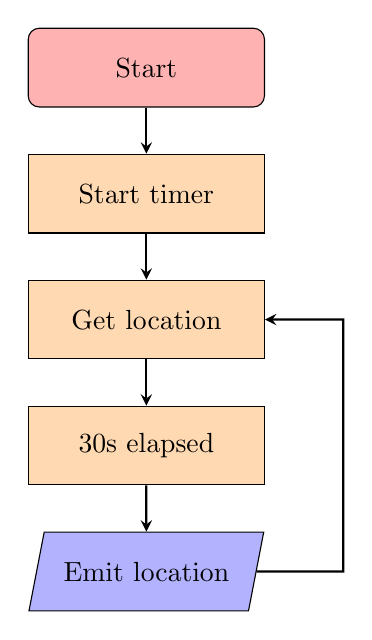
\begin{tikzpicture}
            \node (start) [startstop] {Start};
            \node (timer) [process, below of=start, yshift=-0.6cm] {Start timer};
            \node (loc) [process, below of=timer, yshift=-0.6cm] {Get location};
            \node (elapse) [process, below of=loc, yshift=-0.6cm] {30s elapsed};
            \node (emit) [io, below of=elapse, yshift=-0.6cm] {Emit location};

            \draw [arrow] (start) -- (timer);
            \draw [arrow] (timer) -- (loc);
            \draw [arrow] (loc) -- (elapse);
            \draw [arrow] (elapse) -- (emit);
            \draw [arrow] (emit) -- ++(2.5,0) |- (loc);
        \end{tikzpicture}
        \caption{Transmitter}
    \end{subfigure}\quad
    \begin{subfigure}{.4\textwidth}
        \centering
        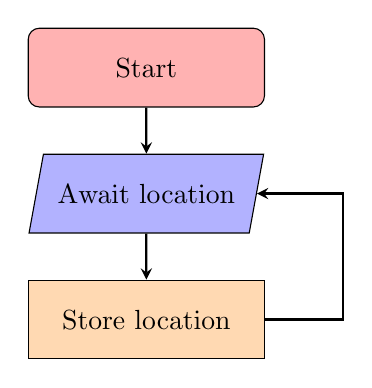
\begin{tikzpicture}
            \node (start) [startstop] {Start};
            \node (inp) [io, below of=start, yshift=-0.6cm] {Await location};
            \node (store) [process, below of=inp, yshift=-0.6cm] {Store location};

            \draw [arrow] (start) -- (inp);
            \draw [arrow] (inp) -- (store);
            \draw [arrow] (store) -- ++(2.5,0) |- (inp);
        \end{tikzpicture}
        \caption{Receiver}
    \end{subfigure}    
    \caption{System overview flowchart}
    \label{fig:system overview flowchart}
\end{figure}

\subsection{Hardware}

Given the specification list, some hardware requirements can be defined to inform purchasing decisions.
The transmitter needs to be portable, therefore each component is size, weight, and power limited. The receiver,
on the other hand, is designed to be stationary and has no technical size or power limitations. However, 
it has to be sized within reason for a product designed for home use.

The following component list will help inform what specific components are required, which has been 
drawn into a hardware block diagram in \cref{fig:hardwareblockdiag} to aid visualisation. 
\begin{itemize}
    \item Transmitter
          \begin{itemize}
              \item \acrshort{gps} module for location.
              \item \gls{lora} module for transmission.
              \item Small form-factor antenna to aid transmission.
              \item Microcontroller for general computation.
              \item Battery as a remote power source.
          \end{itemize}
    \item Receiver
          \begin{itemize}
              \item \gls{lora} module for transmission.
              \item Microcontroller or \acrshort{sbc} for computation.
          \end{itemize}
\end{itemize}

% \begin{figure}[htbp]
%     \centering
%     \begin{subfigure}[b]{0.475\textwidth}
%         \centering
%         \includegraphics[height=5cm, keepaspectratio]{../figures/mcblock.png}
%         \caption{Transmitter}
%     \end{subfigure}
%     \hfill
%     \begin{subfigure}[b]{0.475\textwidth}
%         \centering
%         \includegraphics[height=5cm, keepaspectratio]{../figures/sbcblock.png}
%         % \includesvg[inkscapelatex=false,width=\textwidth]{../figures/sbcblock.svg}
%         \caption{Receiver}
%     \end{subfigure}
%     \caption{Hardware block diagram}
%     \label{fig:hardwareblockdiag}
% \end{figure}

\begin{figure}[H]
    \centering
    \begin{subfigure}[b]{0.625\textwidth}
        \centering
        
        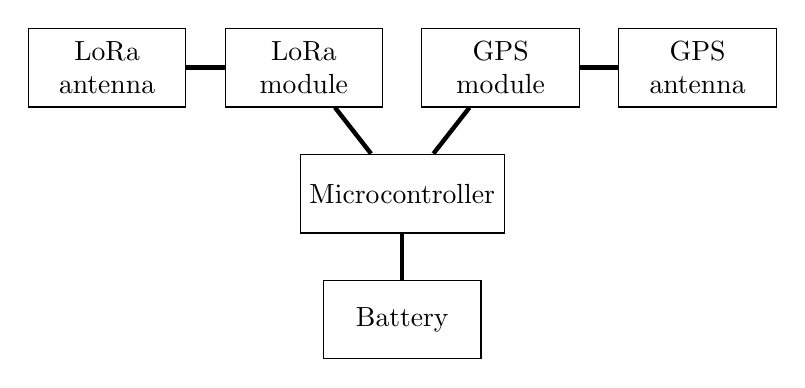
\begin{tikzpicture}        
            \node (mc) [rec] {Microcontroller};
            \node (lora) [rec, above of=mc, yshift=0.6cm, xshift=-1.25cm] {LoRa\\module};
            \node (loraant) [rec, left of=lora, xshift=-1.5cm] {LoRa\\antenna};            
            \node (gps) [rec, above of=mc, yshift=0.6cm, xshift=1.25cm] {GPS\\module};
            \node (gpsant) [rec, right of=gps, xshift=1.5cm] {GPS\\antenna};
            \node (batt) [rec, below of=mc, yshift=-0.6cm] {Battery};

            \draw [bar] (mc) -- (lora);
            \draw [bar] (lora) -- (loraant);
            \draw [bar] (mc) -- (gps);
            \draw [bar] (gps) -- (gpsant);
            \draw [bar] (batt) -- (mc);
        \end{tikzpicture}

        \caption{Transmitter}
    \end{subfigure}
    \hfill
    \begin{subfigure}[b]{0.325\textwidth}
        \centering
        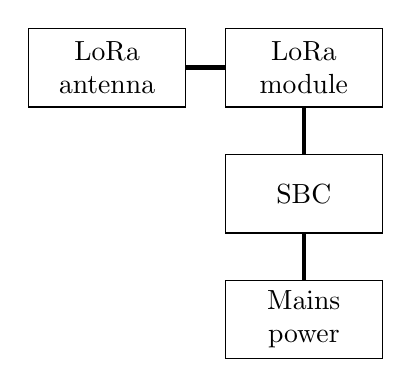
\begin{tikzpicture}        
            \node (sbc) [rec] {SBC};
            \node (lora) [rec, above of=sbc, yshift=0.6cm] {LoRa\\module};
            \node (loraant) [rec, left of=lora, xshift=-1.5cm] {LoRa\\antenna};   
            \node (pwr) [rec, below of=sbc, yshift=-0.6cm] {Mains\\power};

            \draw [bar] (sbc) -- (lora);
            \draw [bar] (lora) -- (loraant);
            \draw [bar] (pwr) -- (sbc);
        \end{tikzpicture}      

        \caption{Receiver}
    \end{subfigure}
    \caption{Hardware block diagram}
    \label{fig:hardwareblockdiag}
\end{figure}

There are many possible configurations to produce the sets of hardware required 
from parts available across different vendors. With this in mind, solutions that 
incorporate built-in features will be prioritised.

\subsubsection{SBC choices}
Some decisions were made to narrow down the diverse range of options, given hardware 
availability and technological experience. Regarding the transmitter controller;
while this may be as simple as a microcontroller, with extensibility and future-proofing 
in mind\footnote{
    For example, serving a user-interface, storing data in a database etc.
}, an \acrshort{sbc} will be the product of focus. Given hardware shortages,
should there be none available, this may be revisited. 
There are a number of \acrshort{sbc} offerings available, some of which are listed 
with a discussion in \cref{table:sbc}.

{\small
\begin{xltabular}{\linewidth}{|Z|Z|Z|Z|}
    \hline
    \rowcolor{tableh2}
    Board & Description & Benefits & Drawbacks \\
    \hline
    Raspberry Pi        & A series of general purpose \acrshortpl{sbc} using Broadcom BCM series \acrshortpl{soc}. 
        & \textbullet Inexpensive \newline \textbullet \acrshort{gpio} \newline \textbullet Pi 3 available
        & \\
    \hline
    NVIDIA Jetson Nano  & AI and neural network development focused, built around the ARM Cortex-A57 and NVIDIA Maxwell.                                       
        & \textbullet Powerful \newline \textbullet \acrshort{gpio}
        & \textbullet Expensive \newline \textbullet More powerful than necessary \newline \textbullet Availability \\ 
    \hline
    Beaglebone Black    & Pi equivalent, using an ARM Cortex-A8.                              
        & \textbullet Inexpensive \newline \textbullet \acrshort{gpio}
        & \textbullet Availability \\
    \hline
    Dell Wyse           & Thin client server/PC.
        & \textbullet Familiar interface for an end user \newline \textbullet Easier \acrshort{gui} programming  
        & \textbullet No \acrshort{gpio} \newline \textbullet Very expensive \\
    \hline
    \caption{\Acrshort{sbc} considerations}\label{table:sbc}
\end{xltabular}
}

With all things considered, the Raspberry Pi is the most obvious choice simply
from the standpoint that a Pi 3 is currently available for use. 
Given the current climate, it is virtually impossible to order computing hardware in this category. Even the Pi Compute
Modules, small form-factor Pi boards with no peripherals or breakouts, are often out of stock. This is despite the fact that 
these boards are unable to function `out of the box'. 

\subsubsection{Microcontroller choices}
The transmitter does not need to perform anything greater than obtaining \acrshort{gps} coordinates 
and transmitting them by \gls{lora} radio. For this reason, a microcontroller is well suited. 
There is an even greater selection available than with the \acrshort{sbc} choices. Therefore, 
as before, the options will be shortlisted and considered in \cref{table:mc}.
\clearpage

{\small
\begin{xltabular}{\linewidth}{|Z|Z|Z|Z|}
    \hline
    \rowcolor{tableh2}
    Board & Description & Benefits & Drawbacks \\
    \hline
    Arduino Uno & One of the most popular microcontrollers available, with an ATmega328P at its core. 
        & \textbullet Widely available \newline \textbullet Large peripheral and software support 
        & \textbullet Large \\
    \hline
    Challenger RP2040 LoRa & Embedded computer with integrated LoRa modem using the RP2040, a dual ARM Cortex-M0+ microcontroller. 
        & \textbullet Integrated \gls{lora} modem 
        & \\
    \hline
    Feather RP2040 & RP2040 board produced by Adafruit in the feather form-factor.
        & \textbullet Feather form-factor \newline \textbullet USB-C
        & \\
    \hline
    Wio-E5 mini & Compact LoRa dev board produced by Seeed Studio using an STM32WLE5JC, a bundled ARM Cortex-M4 microcontroller and SX126X \gls{lora} radio modem.
        & \textbullet Integrated microcontroller and \gls{lora} modem \newline \textbullet USB-C
        & \textbullet Availability \newline \textbullet Involved programming requirements\\
    \hline
    Feather 32u4 with LoRa & Feather form-factor board with LoRa produced by Adafruit, sporting an ATmega32u4.
        & \textbullet Integrated \gls{lora} modem \newline \textbullet Prior experience \newline \textbullet Feather form-factor
        & \textbullet Availability \\
    \hline
    \caption{Microcontroller considerations}\label{table:mc}
\end{xltabular}
}

The board of choice here would be the Feather RP2040. While integrated \gls{lora} 
is certainly beneficial, having the flexibility to customise it during development 
may prove more helpful\footnote{
    The RFM95W \gls{lora} chipset uses \acrshort{spi} and has, in previous experience,
caused difficulties with hardware on the same bus. In case it is necessary, an alternative set
of hardware using the \acrshort{i2c} bus will be produced.
}. Furthermore, this board shares the advantage of other Feather 
boards in that they are stackable, meaning Adafruit's large range of peripherals 
(including \gls{lora} Featherwings and \acrshort{gps} Featherwings) are available to use. 

Purchasing two such \gls{lora} Featherwings for use in the transmitter and receiver 
ensures they are able to communicate with each other without issue. Given the selected 
form-factor and subsequent ease of use, it follows that the \acrshort{gps} module will be 
from Adafruit's Featherwing line. 

\subsection{Purchasing}

Some antenna options will be included as the best approach 
for this has not yet been determined. Ceramic antennae have the smallest form-factor,
however they may prove difficult to mount due to small contact points compared to more traditional 
wire antennae. The receiver will also require a large gain antenna to pick up weak transmissions.

A preliminary hardware set was produced\footnote{
    \Cref{table:prelimhardwarelist}.
}. This list consists 
of two sets of hardware for the transmitter, hardware required regardless of set, and some antenna 
options. 

The radios selected use the same model modem, the RFM95W \cite{hoperf:rfm95w}, 
ensuring the modules are capable of communicating (i.e. are operating within the 
same wavelength range).

\paragraph{Order review}
The list had to be adjusted to primarily target hardware from approved vendors\footnote{
    \Cref{table:updatedhardwarelist}.
}. 
With the vendor adjustment made, some of the initial hardware had to be substituted for 
more expensive alternatives. This made board options simpler by limited the feasible solution
to a Feather M0 with bundled \gls{lora} modem. Additional accessories were included, along with 
an extensive set of antenna and battery options to choose from. 

This list was further adjusted to omit spare hardware that is available to use (for example, 
headers, connectors, etc.). Furthermore, battery purchasing will be put on hold until 
the required capacity can be determined. Finally, the \gls{lora} module for the Pi was 
changed to a \acrshort{hat}. This uses the same radio hardware, but has the additional benefit 
of being able to directly interface with the Pi pins. 
The list was then requested for purchasing. 


 % 7 pages

\section{Development}
\subsection{Initial function}
This section concerns getting the tracker to the point where it can transmit \acrshort{gps} location 
via \gls{lora}.
\subsubsection{Hardware}
The Feather (M0 \gls{lora}) and \acrshort{gps} Featherwing are designed to
be directly stackable\footnote{
    \Cref{fig:gpstack}.
}, and as such share the same pin placement and 2D dimensions. 
The pinout diagram for the Feather M0 can be found 
in \cref{fig:m0pinout}, with matching pin placement for the \acrshort{gps} Featherwing 
in \cref{fig:gpspin}.

Therefore, each pin can be soldered directly using included headers.
For now, additional hardware like batteries and antennae are not necessary, as only
basic function will be tested. 

The Pi \acrshort{hat} is similarly configured to slot onto the \acrshort{gpio} pins
available on the Pi 3 directly. Pinout diagrams for the board can be 
found in \cref{fig:raspipinout}. No additional work is required to interface the hardware.

\subsubsection{\acrshort{gps}}
\label{sec:devgps}
With the boards soldered together, basic operation can be checked 
by loading the `blink' sketch \cite{arduino:blink} using Arduino's \acrshort{ide}.
This sketch will simply switch the inbuilt LED on and off every second, and can be used to verify that
the board can accept and run sketches.

\begin{wrapfigure}[11]{R}{0.6\textwidth}
    \vspace{-5pt}
    \centering
    \captionsetup{justification=centering}
    \includegraphics[width=0.6\textwidth]{../figures/hardwareserialoutput.png}
    \caption[GPS hardware serial output]{\acrshort{gps} hardware serial output with sensitive location data censored,
        showing \gls{gprmc} and \gls{pgtop} sentences.}
    \label{fig:gpshardwareserial}
\end{wrapfigure}


Having proven basic function, the next test concerns the function of the specific hardware. The \acrshort{gps} module
will be focused on to begin with.

The initial test sketch as per the documentation \cite{adafruit:gps, adafruit:gpshardwareserial} is loaded.
This produces output as in \cref{fig:gpshardwareserial}.
% \begin{figure}[H]
%     \centering
%     \captionsetup{justification=centering}
%     \includegraphics[width=0.5\textwidth]{../figures/hardwareserialoutput.png}
%     \caption[GPS hardware serial output]{\acrshort{gps} hardware serial output with sensitive location data censored,
%         showing \gls{gprmc} and \gls{pgtop} sentences.}
%     \label{fig:gpshardwareserial}
% \end{figure}

By default, the \acrshort{gps} module outputs many standardised \acrshort{nmea} sentences,
the most important of which to begin with is the \gls{gprmc} sentence.

\begin{lstlisting}[label=code:gprmcsentence, caption={\acrshort{nmea} \gls{gprmc} sentence example},captionpos=b]
$GPRMC,224029.000,A,5223.00,N,00133.00,W,0.91,44.23,140123,,,A*40
\end{lstlisting}

The output format is not immediately obvious. The \cref{code:gprmcsentence} can be broken down as follows \cite{baddeley:nmea, novatel:gprmc}:
\begin{description}[align=left, labelwidth=2.5cm,labelindent=1cm]
    \item[\gls{gprmc}] Message ID
    \item[223029.00] Time in UTC (22:30:29.00)
    \item[A] Validity - \textbf{A}ctive/\textbf{V}oid
    \item[5223.00,N] Latitude (52\textdegree23.00'' North\footnote{The longitude and latitude appear to be in
            decimal degrees at a glance and will therefore return errors when attempting to plot with this expectation.
            Furthermore, it is specifically degrees minutes and not degrees minutes seconds as one may expect.})
    \item[00133.00,W] Longitude (001\textdegree33.00'' West)
    \item[0.91] Speed (knots)
    \item[44.23] Tracking angle
    \item[140123] Date (14\textsuperscript{th} January 2023)
    \item[A] Positioning mode indicator 
        \begin{description}[align=left, labelwidth=1cm,labelindent=2.75cm]
            \item[A] Autonomous
            \item[D] Differential
            \item[E] Estimated (dead reckoning)
            \item[M] Manual input
            \item[N] Data not valid
        \end{description}
    \item[40] Checksum (XOR of all bytes between \$ and *)
\end{description}

The output location was verified to be correct. Obtaining a fix while indoors proved very difficult. The \acrshort{gps} module uses
coin cell to save fix data, which would have helped obtain a fix outdoors and then move indoors to observe the data.

The \gls{pgtop} sentence characterises the antenna connection, a non-standard command specific to the FGPMMOPA6H module \cite{gtop:pa6h}.
\begin{lstlisting}[label=code:pgtopsentence, caption={\acrshort{nmea} \gls{pgtop} sentence example},captionpos=b]
    $PGTOP,11,2*6E
\end{lstlisting}
\Cref{code:pgtopsentence} can be broken down as follows:
\begin{description}[align=left, labelwidth=2cm,labelindent=1cm]
    \item[\gls{pgtop}] Message ID
    \item[11] Command ID
    \item[2] Antenna status
        \begin{description}[align=left, labelwidth=0.75cm,labelindent=2.25cm]
            \item[1] Active antenna shorted
            \item[2] Using internal antenna
            \item[3] Using external (active) antenna
        \end{description}
    \item[6E] Checksum
\end{description}

The antenna status is not particularly useful, especially so at this stage of the development.
Therefore, it can be disabled. Many of the commands to program the device (for example,
changing the sentence output frequency) can be found in the \gls{pmtk} reference document\footnote{
    With a battery, the \gls{pmtk} commands are retained and do not
    need to be presented to the module on power-on. Otherwise, settings must be reconfigured on
    every boot.} \cite{gtop:pmtk}.
Alternatively, the Adafruit \acrshort{gps} library \cite{adafruit:gpslibrary} has support for some commands.
These commands are not documented and can only be found hardcoded into the header file of the
library \cite{adafruit:gpspmtk}.

Regarding the antenna, it can be disabled in two ways, via serial\footnote{This must be the serial
    connection to the \acrshort{gps} device from the main board, and cannot be accessed directly via serial monitor.
    In order to send commands on the fly via serial monitor, the code must be configured to then forward those commands
    to the correct serial connection (in the case of \cref{code:pgtopdisableserial}, `serial1').} :
\begin{lstlisting}[label=code:pgtopdisableserial, caption=\relax,captionpos=b]
    #define GPSSerial Serial1
    GPSSerial.println("$PGCMD,33,0*6D");
\end{lstlisting}
or using the library:
\begin{lstlisting}[label=code:pgtopdisablecmd, caption=\relax,captionpos=b]    
    Adafruit_GPS GPS(&GPSSerial);
    GPS.sendCommand(PGCMD_NOANTENNA);    
\end{lstlisting}

The library provides some useful functions and makes the code less verbose and more readable,
however it may prove to include significant enough overhead to impact the battery life.
If that happens to be the case the library can be removed as essential function
can be programmed to the \acrshort{gps} chip directly via serial.

\subsubsection{Pi \gls{lora}}
The \gls{lora} bonnet library as provided by Adafruit requires Circuit Python to be installed
on the Pi \cite{adafruit:circuitpython,adafruit:lorabonnet}\footnote{The installation documentation
    concerns both RFM69 and RFM9X radios. This project uses the RFM95W radio, also referred to
    as \gls{lora}.}.

With required software, libraries, and fonts installed, the example code \cite{adafruit:rfm95check}
can be loaded. This checks that the radio is present and the \acrshort{oled} displays correctly.

Finally, the radio function script can be loaded \cite{adafruit:radiopy}. This will await
incoming \gls{lora} packets, but can also send data using the buttons.

\subsubsection{Feather \gls{lora}}

\gls{lora} transmission with this board relies on the RadioHead library \cite{airspayce:main} in order to
transmit \gls{lora} packets, installation details for which can further be found in the
documentation \cite{adafruit:loram0}.

The transmission test script can be loaded onto the Feather \cite{adafruit:feathertx} once required software
has been installed. This will transmit a packet every second and await a reply.
For the time being, the Pi will not automatically send a reply, so the Feather will output
the ``error text''. This is of little consequence as the Pi
primarily only needs to work as a receiver with no two-way communication\footnote{The test script on the
    Pi does in fact allow output by pressing one of the buttons. This can be used to test communications
    and will be picked up by the Feather if this is tested.}.

\subsubsection{\gls{lora} with \acrshort{gps}}
With one-way communication working as expected\footnote{Both example scripts are set at \qty{915.00}{\MHz}
    and will work by default. This needs to be adjusted to \qty{868.00}{\MHz} for use in the UK
    \cite{ofcom:licenceexempt}.}, the next step is to integrate \gls{lora} with \acrshort{gps} on the Feather. This
stage is where communication collision issues have occurred in previous projects,
however as the \acrshort{gps} module uses the second serial connection and the \gls{lora} chip uses \acrshort{spi}, no such
issues should occur.

For streamlined testing, the library will be used to strip the data sent to only latitude, longitude, and packet number
(incremented every time \acrshort{gps} location is fixed to indicate that the location is up-to-date). The various
segments of data then need to be placed together in a structure. The public member function \lstinline{send()} of the
\lstinline{RH_RF95} class \cite{airspayce:docs} takes two arguments, \lstinline{data (uint8_t*)} and \lstinline{len (uint8_t)}.
This means that the data to be sent needs to be consolidated into a single structure, with the pointer to the structure
and its length sent to the function. The Arduino compiler is built on processing AVR-C and therefore suffers when handling
strings and performing conversion and concatenation natively, which can lead to complex and verbose code.
The Arduino \acrshort{ide} also supports C++ classes and function, amongst which
include the \lstinline{String} class and \lstinline{+} concatenating function
\cite{arduino:introduction, arduino:reference}. While the class may prove problematic on embedded hardware
due to memory fragmentation on the heap, for the time being it is sufficient where the primary goal is
functional and readable code. Two additional benefits are that the length is also easily attainable
as the method \lstinline{.length()} on the class, and also conversion to an array of type \lstinline{char} is supported.
\Cref{code:transmissionbody} shows a snippet of the body code.

\begin{lstlisting}[language=C++,label=code:transmissionbody,caption={Transmission body code},captionpos=b]
void loop() {
    //buffer gps location
    char c = GPS.read();           
    //interpret whether new location obtained and parse
    if (GPS.newNMEAreceived()) {    
        if (!GPS.parse(GPS.lastNMEA())) { 
            return;
        }
    }
    //execute every 5 seconds
    if (millis() - timer > 5000) {  
        timer = millis(); 
        //increment packet counter if new fix obtained
        if (GPS.fix) {
            count++;                
        }
        //produce concatenated string
        String output = String(count) + ": " + String(GPS.latitude,4) + "," + String(GPS.longitude,4);      
        length = output.length();
        //create variable send to hold packet once converted to type char
        char send[length];          
        output.toCharArray(send, length);
        Serial.println(send);   
        rf95.send((uint8_t *)send, length);        
    }
}
\end{lstlisting}

The output can be observed in \cref{fig:loraoutput}, showing \gls{lora} and GPS working together.

\begin{figure}[H]
    \label{fig:loraoutput}
    \begin{subfigure}{0.45\textwidth}
        \centering
        \includegraphics[height=4cm]{../figures/feather tx.png}
        \caption{Feather transmission logs}
    \end{subfigure}
    \hfill
    \begin{subfigure}{0.45\textwidth}
        \includegraphics[height=4cm]{../figures/pi rx.png}
        \caption{Pi reception logs}
    \end{subfigure}
    \caption[LoRa communications with GPS location]{\gls{lora} communications with \acrshort{gps} location}
\end{figure}

\subsection{Power tester}
In order to determine the appropriate battery capacity to use, it is helpful to test the power consumption
of the transmitter over the expected period of use. Greater capacity batteries are heaver and larger - two
factors that need to be minimised. There is also the potential fire risk, however this is minimal without damage. 

By recommendation, a KCX-017 \acrshort{usb} tester was purchased to measure the current draw of the transmitter under
normal function. The included manual was poorly translated and difficult to follow, however a more
informative version was found online \cite{kcx}. No further details about the manufacturer or
any other products they may produce were found.

\subsubsection{Test specification}
\label{sec:powertestspec}
The outline of the test is to determine the appropriate battery required for the module. The tester
has various functions available, however only the capacity recording is relevant. The tester will
be plugged into a \acrshort{usb} outlet, and the transmitter will be plugged into the tester. The transmitter
will be plugged into the tester and will operate from thereon. Recordings will be taken every thirty
minutes for four hours as a preliminary measure of function. The Pi will be running to record
that the transmitter is operating as expected.

Two tests were performed:
\begin{enumerate}
    \item The transmitter was housed indoors so that it is unable to obtain a \acrshort{gps} lock. This
          will lead to the greatest power consumption.
    \item The transmitter was placed near a window so that it is able to update \acrshort{gps} location.
          This simulates normal operation.
\end{enumerate}

\paragraph{Risks}
The only identifiable risk is excessive current draw for the tester to handle. 
This risk is negligible as the tester is quoted to have a current limit 
of \qty{3500}{\mA} \cite{kcx},
which is far beyond the Feather capabilities. 

\subsubsection{Results}
Upon commencing the first test, the receiver registered no data. The cause was to simply
remove the line \lstinline{while (!Serial) delay(10);} as it prevents the code executing
until the serial interface is connected, so output can be monitored. In the case of this test,
serial output was not required, however the line still stalled the code.

With the change made and output occurring as expected, the meter did not appear to
register any changes. The meter was checked to be working by observing the current 
draw of a mobile phone, and was found to be operating as expected.
Thereafter, the meter was left and checked every hour.
The first change only occurred after three hours.

The consumption incremented only after three hours. It was left overnight and checked again,
at this point registering \qty{8}{\mAh}. The complete set of recordings
can be found in \cref{table:powermeter}. The data is plotted below using
code in \cref{script:powermeter}.
\begin{figure}[H]
    \centering
    \label{fig:powermeter}
    \includegraphics[width=\textwidth]{../../Tests/power meter/powermeter.png}
    \caption{Power meter results}
\end{figure}

The results suggest that, during normal operation, the transmitter requires around only
\qty{0.5}{\mA}. This is far too low to be accurate, and in turn,
likely means the meter does not have sufficient resolution
to measure the device. The meter does indicate a linear trend in power draw
suggesting predictability in normal use,
however given the poor accuracy of the data, the validity of this cannot be determined.

\subsection{Intermediate steps}
\label{sec:intermediate}
The power meter results were disappointing, however the documentation for the hardware
provides useful values with which an estimated battery capacity requirement can be produced.
The \gls{lora} board draws \qty{40}{\mA} when the radio is actively
listening, and draws \qty{130}{\mA} for \qty{70}{\ms} when transmitting at peak gain \cite{adafruit:loram0}.
The \acrshort{gps} module draws \qty{25}{\mA} when tracking and \qty{20}{\mA} during navigation \cite{adafruit:gps}.
This gives a rough total of \qty{60}{\mA} typical draw in the average case. Considering the
transmitter needs to operate for nine hours\footnote{\Cref{sec:specsbatt}.},
this suggests a battery capacity requirement of \qty{540}{\mAh}.

This suggests that a repurposed \qty{3.7}{\V}
\qty{500}{\mAh} quadcopter battery, may be used to test the transmitter functionality directly.
The \gls{lora} board requires a JST jack \cite{adafruit:loram0}. By investigating Adafruit's
other products, this appears to be a JST-PH connector specifically \cite{adafruit:jst}.

The battery header was removed and a JST-PH connector crimped onto the end of the leads.
The polarity was then checked before powering the transmitter and ensuring it functioned
as before.

\subsubsection{Code issues}
\label{sec:codeissues}
During such a function test, the code on the receiver end crashed twice, producing an error such
as in \cref{code:programerror}.

\begin{lstlisting}[caption={Program error message},label=code:programerror,captionpos=b]
Traceback (most recent call last):
    File "/radio.py", line 72, in <module>
        packet_text = str(prev_packet, "utf-8")
UnicodeDecodeError: 'utf-8' codec can't decode byte 0xae in position 0: invalid start byte
\end{lstlisting}

Due to the module being powered up and disconnected abruptly multiple times
while setting up the battery, the suspicion was that transmission was interrupted midway,
leading to the receiver attempting to parse an unfinished and corrupted packet. However,
given the time window of less than \qty{100}{\ms} for transmission, the fact this occurred
twice suggests this theory may not be likely.

In order to test how long the transmitter is able to function, the code needs to be
improved to be more resilient and stable. The example code \cite{adafruit:radiopy} has
been updated to safely handle the exception. While the cause of the error has not been
determined or investigated further at this point, the code will now attempt to parse
the packet in a \lstinline{try/except} block. The first handles the
\lstinline{UnicodeDecodeError} directly, while the second handles anything else that
may occur, in case there are other issues that have not been uncovered. It will indicate
that an unexpected error has occurred and continue execution from thereon.
The modified code can be found in \cref{pi:radio}.

\subsubsection{Antenna}

\begin{wrapfigure}{R}{0.4\textwidth}
    \centering
    % \captionsetup{justification=centering}
    \includegraphics[width=0.4\textwidth]{../figures/damaged antenna.jpg}
    \caption{Damaged strip antenna.}
    \label{fig:damagedantenna}
\end{wrapfigure}

Due to delivery issues, neither module currently is able to use an antenna, and thus have
been confined to short range tests only.
While part of the purchasing list included ceramic and strip antennae for the
transmitter only, the ceramic antennae cannot be used as they require some form of breakout,
usually on a \acrshort{pcb} and further currently require a \gls{ufl} adapter to interface
with the board. The strip antenna, on the other hand, use a very delicate cable between the strip itself and
the connector, and were therefore easily sheared by one \textit{Felis catus} who found it
unattended during operation.

% \begin{figure}[H]
%     \centering
%     % \captionsetup{justification=centering}
%     \includegraphics[width=0.4\textwidth]{../figures/damaged antenna.jpg}
%     \caption{Damaged strip antenna.}
%     \label{fig:damagedantenna}
% \end{figure}

A spare whip antenna was available to use with the Pi, however its frequency was
unknown. Upon casual inspection, it may be appropriately sized. To investigate further,
the appropriate antenna length needs to be determined.

The wavelength can be found by:
\begin{align*}
    \lambda & = \frac{v}{f}
\end{align*}

\begin{conditions}
    \lambda & = & wavelength \\
    v & = & velocity, which in this case will be $c$, the speed of light \\
    f & = & frequency \\
\end{conditions}

% where: 

% \begin{tabular}[H]{ l c l}
%     $\lambda$ & $=$ & wavelength \\
%     $v$ & $=$ & velocity, which in this case will be $c$, the speed of light \\
%     $f$ & $=$ & frequency \\
% \end{tabular}\\

For the device operating at \qty{868.0}{\MHz}, this appears like the following:
\begin{align*}
    \lambda & = \frac{c}{\qty{868.0}{\MHz}} \\
            & = \qty{0.345}{\m}
\end{align*}

The antenna whip measures between \qty{21}{\cm} and \qty{25}{\cm}, although
it is impossible to say exactly how long it is without opening it up.
If this antenna is centred near \qty{868}{\MHz}, it may be a five-eighth whip, given
$\frac{5}{8}\lambda = \qty{21.5}{\cm}$. This suggests it is appropriate to use until 
a more robust set of antennae has requested for ordering\footnote{
    Decided list can be found in \cref{table:antennaelist}.
}.

\subsection{Battery test}

The purpose of the test is to determine the length of time the transmitter can continuously
operate under normal conditions, i.e. obtaining current \acrshort{gps} location and
transmitting it via \gls{lora}.
As outlined in \cref{sec:powertestspec}, there is an expectation of roughly eight
hours of function. This will now be investigated to determine whether this is the case.

The transmitter code will need to be updated to include information about the current
status of the battery. The voltage level of the battery indicates whether it is
within operating range, which can be measured by reading the analogue value of
pin \lstinline{A7}. At \qty{4.2}{\V}, capacity as it maximum, whereas the board
will cease function around \qty{3.2}{\V}. The exact calculation can be found in
the board documentation \cite{adafruit:loram0}, which has been adapted in \cref{arduino:bat}.

After ascertaining that the calculation was working correctly, the code has been included in
\cref{arduino:lpgps2}\footnote{
    This is in fact the third iteration of code. The two former versions can be found in \cref{arduino:serialgps} and \cref{arduino:libgps}.
}. The output string has also been modified to include the battery data,
altitude, and fix quality.
\acrshort{gps} fix takes the following values \cite{arcgis:gpsfix}:

\begin{description}[align=left, labelwidth=1cm,labelindent=0.5cm]
    \item[0] No fix (no signal)
    \item[1] Position fixed with \acrshort{gnss} satellites
    \item[2] Differential \acrshort{gps}
    \item[3-5] \acrshort{pps}\footnote{Encrypted military/government use}/\acrshort{rtk} fix
    \item[6] Estimated location
        \label{table:fix}
\end{description}

The latter two
required \gls{gpgga} data, which can be included with the library command
\lstinline{PMTK_SET_NMEA_OUTPUT_RMCGGA}. Finally, field separators were replaced with commas
as part of preparation for the data to be stored in \acrshort{csv} format.

\subsubsection{Test parameters}
Two tests were conducted.
\begin{enumerate}
    \item Discharge - The board operates under normal conditions. The battery was
          charged to maximum capacity (\qty{4.2}{\V}), before being allowed to discharge
          completely. Throughout that time, the board was transmitting
          location data and battery level. The receiver logs the time of
          packets and stores it in a data structure.
    \item Charge - After a complete discharge, the time taken to charge to maximum
          was recorded similarly.
\end{enumerate}

The way the Pi is operated was changed. Normally, an \acrshort{ssh} session
is terminated when the client disconnect or times out, and any programs run during that
session are closed. This was not a problem with the
power meter test as the receiver only needed to indicate that transmitter was working,
while the data itself was recorded externally. In this case, the Pi is recording all data
and needs to be running without interruption for at least eight hours.
Linux comes with a utility named
\lstinline{screen} that allows a virtual terminal session to be started that will
not be closed\footnote{An alternative
    would be to run the process and move it to background. The benefit of \lstinline{screen} is that
    logging messages are easier to view when printed to terminal.}.

\paragraph{Risks}
The greatest risk is related to the battery short-circuiting, however this 
has been dealt with adequately in \cref{sec:intermediate}. 
It is possible the battery may be damaged due to excessive discharge,
however the protection circuitry will cut the supply before then. 

\subsubsection{Issues}
The tests were executed without issue and a brief study of the results indicated they
were within expectation. However, some issues cropped up.

C treats strings as an array of type \lstinline{char} and determines
the end of the string with the `null' character\footnote{In two byte
    hexadecimal representation as an escape character, \lstinline{\\x00}.} `\lstinline{\0}'.
C++ carries this over. Thereby, when using the C++ \lstinline{String} class,
this behaviour remains. As it is treated as part of the string, it is furthermore
included in the length calculation and therefore transmitted over \gls{lora}.
The receiver would then interpret the characters of the packet in \lstinline{utf-8},
and translate the null character as \lstinline{\x00}. The existence of null characters
introduces difficulty when attempting to interpret the file in \acrshort{csv} format.

The eventual solution was to perform packet processing on receipt, 
as cleaning the files manually had thus far failed.
The inbuilt \lstinline{rstrip()} method on a string type allows a specific character
(in this case, \lstinline{\x00}) to be removed. 

Additionally, supplementary information, like errors, were logged to console
with extra diagnostic information instead of stored in the file.
Beforehand, this information would have to be stripped as the error line was non-standard for
the \acrshort{csv} format\footnote{
    The producing code can be found in \cref{pi:first}.
}. An example is shown in \cref{table:errorlogex}.

{\small
\begin{xltabular}{\linewidth}{|ccllll|}
    \hline
    \rowcolor{tableh1}
    Date & Time & Packet & Longitude & Latitude & Voltage \\
    \hline
    23/01/27    & 20:27:27  & 3040  & 0	    & 0  & 4.15  \\
    23/01/27	& 20:27:32	& 3041	& 0     & 0  & 4.15  \\
    23/01/27	& 20:27:35	& unicode parse error & & &  \\
    23/01/27	& 20:27:32	& 3041  & 0     & 0  & 4.15  \\
    23/01/27	& 20:27:37  & 3042	& 0	    & 0  & 4.157 \\
    23/01/27	& 20:27:42	& 3043	& 0	    & 0  & 4.15  \\
    \hline
    \caption{Non-standard format example - 230127.csv sample}\label{table:errorlogex}
\end{xltabular}
}

This would cause errors for the \acrshort{csv} interpreter due to mismatched
field lengths.

Finally, plotting temporal data types proved to be problematic.
To simplify this, two changes were made: firstly, the Date and Time fields
were collated into one field in the standard format MATLAB expects\footnote{
    Format: 1\textsuperscript{st} February 2023 at 1:54pm as ``01-02-23 13:54:00''.
}; secondly, a field was added for recording time relative to Unix epoch
(i.e. now completely numeric and linear) in case plotting with such a field
proves simpler.

The tests were then performed a second time.

\subsubsection{Results}
Data samples of the results can be found in \cref{table:dischargedata} and \cref{table:chargedata}.
The resulting plot is shown in \cref{fig:batteryplot} using code in \cref{script:batteryscript2}\footnote{
    This is the second version of plotting code. The first can be found in \cref{script:batteryscript1}.
}.

\begin{figure}[H]
    \centering
    \includegraphics[width=\textwidth]{../../Code/Tests/Battery/Figure_4.png}
    \caption{Battery charge and discharge curves}
    \label{fig:batteryplot}
\end{figure}

The plots show the battery voltage level and whether the \acrshort{gps} has a fix.

\paragraph{Discharge}
Recording starts with a full battery, indicated by \qty{4.2}{\V}. Operation
continues as expected, with \acrshort{gps} location fixed for much of that time.
On two occasions, the fix was recorded at a value of 6\footnote{
    Reference in \cref{table:fix}.
}.
\acrshort{gps} was not unavailable for long enough to indicate whether not having a fix
has any significant impact on battery consumption.
Overall, the data indicates the total useable span of the device is fifteen hours.

\paragraph{Charge}
Notably, the voltage at the point of charging is much lower than was last recorded
when transmission during discharge cut off. The board does in fact continue to draw power.
This ceases when the protection circuitry of the battery cuts supply entirely. This leads to
some parasitic draw in the elapsed time. \acrshort{gps} location fix did not have a
noticeable effect upon charging. Total time to charge to full capacity was around
five hours and thirty minutes.

\paragraph{Remarks}
The discharge results were surprising. The estimate calculation
\cref{sec:powertestspec} returned an expectation of eight hours of function.
Despite being a conservative estimate, the experimentally found value was
almost double this. Furthermore, additional power saving functions like
putting the radio to sleep when not in use were not used, meaning the operating
time of the device can be further increased\footnote{
    Transmission was set at \qty{5}{\s}, which is better than specified in \cref{sec:timing}.
}. 

The time required to charge the module to maximum capacity was
greater than expected. The slow charging time may come down to
a few reasons. The charging regulator built into
the Feather board is current limited to protect the circuitry \cite{adafruit:loram0}.
It is further limited by the maximum current a \acrshort{usb} 2.0 connector can draw
(\qty{100}{\mA}) \cite{axelson:usb}. This can be negotiated to be greater \cite{ftdi:usb}, however,
and certainly many modern devices, particularly mobile phones, utilise some form of rapid charging.

The data collected suggests reliability. Any moment-to-moment fluctuations will be smoothed out
due to the operating time of the module, so further tests
may not be necessary. Furthermore, it is not advisable to repeatedly charge
and discharge lithium cells from maximum to minimum as doing so reduces the lifespan of the cell.

\subsection{Error investigation}
Further insight may be gained on the corrupted packets\footnote{\Cref{sec:codeissues}.}.
The errors recorded before the discharge test was performed can be found in \cref{error:decoding}.
It is notable that there are fewer errors here than in previous tests. The only significant change
was the use of antennae during transmission. To elaborate on the error message, many of the bytes
in the byte array cannot be decoded as they are all invalid \lstinline{utf-8}, not just the start byte.
The structure should follow 8-bits per character, yet some are greater (\lstinline{\x90w}, line 13), use invalid
hexadecimal (\lstinline{\xb8B}, line 13), or are entirely not present (\lstinline{\x89\\22Rs}, line 4).
\begin{itemize}
    \item Invalid hexadecimal - This appears due to the way Python \lstinline{bytearray} is used. Where the
          default decoding (\lstinline{utf-8}) failed, the array
          is encoded as \lstinline{ASCII} and printed to console.
          This leads to non-hexadecimal characters appearing, and likely some of the missing characters also.
    \item Not 8-bits - If, for example, during transmission part of a byte is lost,
          the remainder of the packet will
          fail to decode correctly and appear in different lengths and otherwise non-standard form.
\end{itemize}

\paragraph{Solution}
There is no simple solution to what is essentially the question of how to ensure data integrity
during transmission in a noisy environment. The RadioHead library supports packet confirmations
with the \lstinline{RHReliableDatagram} class. This does not validate the packet
integrity\footnote{A single bit being flipped may still resolve to a valid packet,
    even if the data is no longer accurate.}, but ensures that the packet has arrived. This
solution alone would require some reverse engineering of the \lstinline{recvfromAck} method
in order to use it on the receiver end, however can be used to request retransmission (i.e.
fail to acknowledge the packet) should it arrive corrupted.

An alternative would be to utilise some form of forward error correction, like parity checking.
This has the limitation of increased complexity and computational load on the transmitter,
and is further limited by being able to correct only one error. To adequately cover the
entire transmission, the packet size (and subsequently, radio power draw and processor time)
would increase.

The corrupted packets are few and infrequent enough (only one at a time) that 
they can simply be omitted. As reporting is set to \qty{5}{\s}, up to five 
packets can fail in a row for the specification of \qty{30}{\s} reporting to be met. 
Moving the device to production would require a revisit of handling data integrity.


\subsection{Case design}

In preparation for the distance test, ensuring the electronics were, at minimum,
protected from damage increased in importance. 
The case will be attached to a cat harness or collar as a complete unit (i.e. sewn in),
however this level of integration will be paused until the hardware is moved onto a \acrshort{pcb}
with smaller form-factor. Instead, the purpose of this case design will be to 
provide a protective enclosure for the period of function testing the tracker. 

\begin{wrapfigure}[9]{R}{0.3\textwidth}
    \vspace{-5pt}
    \centering
    \includegraphics[width=0.3\textwidth]{../figures/Pics/bareboard.jpg}
    \caption{Board and battery at the beginning of case development}
    \label{fig:bareboard}    
\end{wrapfigure}

% \begin{figure}[H]
%     \centering
%     \includegraphics[width=0.7\textwidth]{../figures/Pics/bareboard.jpg}
%     \caption{Board and battery at the beginning of case development}
%     \label{fig:bareboard}
% \end{figure}

\Cref{fig:bareboard} shows the board when development of the case started (especially
showing the stacked height).
As can be seen, the connecting wires between the battery and board were a potential
point of failure. Furthermore, in the process of disengaging the battery repeatedly
to remove power and halt battery drain (due to no current off-switch available),
the wire sheath had pulled back to expose the stranded core\footnote{This became
    bad enough that a makeshift cover made from insulting tape was added to ensure the wires
    did not short circuit - as can be seen most clearly in \cref{fig:case1top}.
}.

% \vspace{33pt}
Two key factors drove considerations for the case development:
\begin{itemize}
    \item Due to mismatched sizing between the battery and board, both had to be enclosed, so they
          would not rock about in the casing.
    \item Given the stage in development and likelihood of frequent easy access, the components
          were separated to best allow easy access, even at the expense of the smallest volume possible.
\end{itemize}

\subsubsection{First case}
\paragraph{Design}
The case was modelled in Autodesk Fusion 360 after measurements were taken
of the components. A raised battery platform with rounded
edges was created to hold the battery. The board takes up noticeably less space and
therefore a cage was modelled to house it securely. An arch was included to allow the
battery connection port to remain available. The lid was designed to fit in the casing
recess. Due to the tendency for \gls{fdm} parts to widen when laid, a fillet was
included in the lid lip to allow room for this. Extra space for the power cabled to
come out of the front of the battery was provided.
Finally, holes were added on all vertical
sides to allow an antenna to be routed through wherever most convenient.

Dimensional drawings for the case can be found in \cref{fig:case1dwg}.

\paragraph{Manufacture}
\label{sec:case1manufacture}
The manufacturing method of choice was 3D printing using an Ultimaker 3 \gls{fdm} printer.
In order to print the casing, it would first have to be `sliced' and encoded into \gls{gcode}.
The software chosen to do this was Ultimaker Cura, as it supported Ultimaker printers natively.
Default `fast' settings were used as the casing was a prototype and therefore dimensional
precision is of less importance. Due to large overhangs in the board enclosure, especially at
the battery port, the head movement speed was increased by 15\% in order to bridge the gaps.
Doing so increases the risk of small features like the pillars to fail due to insufficient time
for the layer to cool. The increased bridging capability meant that supports could be disabled,
however the gap for the battery port would have been too large to bridge without supports,
and was therefore modified into an arch to support itself.

\paragraph{Result}
The first print failed due to an extruder blockage towards the end of the first layer
being completed. As this occurred after the period of observation to ensure successful
printing, the issue was only apparent the next day. The result can be seen in \cref{fig:failedprint}.

% \begin{figure}[H]
%     \centering
%     \includegraphics[width=0.7\textwidth]{../figures/Pics/failedprint.jpg}
%     \caption{Failed print}
%     \label{fig:failedprint}
% \end{figure}

\begin{wrapfigure}{L}{0.3\textwidth}
    \centering
    \includegraphics[width=0.3\textwidth]{../figures/Pics/failedprint.jpg}
    \caption{Failed print}
    \label{fig:failedprint}
\end{wrapfigure}

Immediately, a second print was started, but with the print moved to the second extruder.
Images of the board in the successful second print can be found in \cref{fig:case1img}.

\paragraph{Review}
The case turned out to exceed expectations in quality. The battery platform held the battery
in place surprisingly well (likely largely owing to the material of the battery casing).
The board enclosure also worked very well to secure the board. The lid also fit quite securely,
indicating the fillet worked effectively.

As expected, the pillars widened out somewhat. Despite this, the enclosure
top rail was in very good condition, especially including over the battery port - the largest
gap. Relatedly, the arch turned out to be a hindrance
and too troublesome to connect the battery wires through, and was therefore cut off instead. It
was also not centred on the battery port, due to a mistake during the design process where the
measurement was to the centre of the port, whereas the design was dimensioned to the edge of the
port only. Enough space was granted either side of the port to account for such an error,
and therefore came in use.
The cage as a whole did not prove useful, and only made removing the board from the casing more
tedious. It also was a blockage when routing the power cables, leading to no adequate way to
place them without straining them.

\subsubsection{Second case}
\paragraph{Design}
Considering the issues raised in review of the first case design, some changes were made.
The overall style of the first design was retained, with the battery and board placed
side-by-side. While resoldering the board for a flatter profile was preferred, this
was avoided to prevent any unforeseen issues in advance of the distance test and
would be revisited once testing was complete.

Extra space provided for front-facing egress of power
cables from the battery was removed from the design, amounting to \qty{204}{\mm\squared} saved.
To compensate this, a channel was cut into the battery platform for the cables to run.

A major omission from the first design was the charging port, which was now included in
this revision. The antenna hole diameter was doubled to \qty{5}{\mm}.

The board enclosure was removed, and a small fence was used to replace it.

The dimensional drawings can be found in \cref{fig:case2dwg}.

\paragraph{Manufacture}
The same manufacturing process was used as in the first case\footnote{\Cref{sec:case1manufacture}.}.
A finer print setting was used as the print was being left overnight, and therefore the greater
resolution would have no impact on turnaround time. This setting is part of Cura's default presets,
with no modifications made to fine-tune it.

\paragraph{Result}
The print turned out extremely well. Images can be found in \cref{fig:case2img}.

\paragraph{Review}
The first case was not tested with any antennae, so two issues occurred that
were not accounted for.
Despite the antennae holes being enlarged, they were still too small. This may have been due to
collapse of the layers as there were no supports (leading to oval holes that were
too small for the \gls{ufl} connector).
The board `enclosure' interfered with the \acrshort{gps} antenna wire. This can be
seen more clearly in \cref{fig:case2antennaissue}, and overall means that the board
cannot sit flat. The cable will require a relief channel of its own
like the battery wires.

This case is sufficient for testing with, even if the antennae have to be routed
out the lid. The casing with all components weighs in at \qty{55}{\g}.

There are some aspects to be mindful of when designing a third iteration.
If a flat form factor layout can be used by resoldering the boards, there is potential to
allow for a curved, and thereby more ergonomic design, however strain across the connection
must be accounted for.

Attaching to the harness was not considered at all during either of these designs, and will
be a major factor for how guiding the design. Similarly, general weatherproofing was not included.
A simple and effective method of waterproofing would be to use an o-ring as a seal, however this may
require more pressure than the plastic (in this case, \gls{pla}, which is extremely
flexible) is able to provide. This may be mitigated somewhat by using a more rigid material
(for example, \gls{abs} or \gls{pc}) and using screws to secure the lid and apply
the required amount of pressure to form an adequate seal.

Another omission was adequate antenna support. For that reason, during test a flat support
material will be used to protect the antennae. However, this will be an important 
factor with further iterations of case design, especially considering interference sources 
for the antennae being so close to a \acrshort{pcb} edge. 

\subsection{Distance test}
This test forms a crucial part of determining the suitability of the tracker to
perform its key function - tracking a remote target. It is only possible as the
culmination of every step before it.

\subsubsection{Preparation}
This test required more preparation than any performed previously.

\paragraph{Location}
Determining a suitable location for testing was of heightened importance.
The general area to perform the test was decided across the campus of the
University of Warwick. As a publicly accessible space, setting up the receiving
antenna anywhere with thoroughfare would not have been appropriate, however
easy access to the Pi to download data would be needed.

In short, the location needed to be easily accessible, but not in a location
with many people. This ruled out many of the building rooftops due to
potential safety issues and authorisation requirements. The final location
decided was room A3.27, located in the School of Engineering\footnote{
    Location on map: \cref{fig:roomlocation}.
}. This location
was sufficiently high up and had a clear view of Car Park 9 (CP204) and
Lord Bhattacharyya Way. Unfortunately, there was no logistical method with
which the antenna could be mounted outdoors from this location, and therefore
was confined to being indoors. This would severely impact the capability of the antenna.

\paragraph{Work flow}
For ease-of-access, being able to view the data log remotely would be most ideal.
It also means that, should the connection drop out, this can be noticed immediately by
viewing current incoming packets. Remote access requires some manner in which the devices
accessed appears in the `same location'. In this case, it would, in its simplest form,
require a static \acrshort{ip} assignment.
Due to the university network security requirements and address assignment protocol
(likely at best a \acrshort{dhcp} assignment from a limited pool),
there was no ideal way in which the Pi
could be assigned a static \acrshort{ip} address.

The alternative was to set the Pi and antenna up to record data, and retrieve data afterwards.
This comes with the downside that the test can no longer be dynamic. Any issues that occur can
only be investigated after the fact.

With the work flow determined, the setup has the antenna next to a window while connected to the
Pi. A laptop is then connected with an Ethernet cable to the Pi over \acrshort{ssh}.
\Cref{fig:disthardwaresetup} shows a diagram of this hardware setup.

\begin{figure}[htbp]
    \centering
    \begin{subfigure}[b]{0.65\textwidth}
        \centering
        \includegraphics[height=7cm,width=\textwidth,keepaspectratio]{../figures/maps/room.png}
        \caption{A3.27 location, showing Car Park 9 (CP204)}
        \label{fig:roomlocation}
    \end{subfigure}
    \hfill
    \begin{subfigure}[b]{0.3\textwidth}
        \centering
        \includegraphics[height=7cm,width=\textwidth,keepaspectratio]{../figures/maps/setup.png}
        \caption{Hardware setup}
        \label{fig:disthardwaresetup}
    \end{subfigure}
    \caption{Distance test location and setup}
    \label{fig:distancesetup}
\end{figure}

\paragraph{Container}
While the transmitter now has appropriate casing, the antenna holes were too small
to run the \gls{ufl} connector through. Due to time constraints, this could not be
remedied, and instead, the antennae were exposed through the lid.
This also left them with no support, which may prove a point of failure if left unattended\footnote{
    \Cref{fig:case2antennasplay} shows how the antennae splay.
}. To secure the antennae, a scrap sheet of acrylic was used to tape them down, thereby
providing them a rigid support surface with a low chance of leading to interference.
The final result of the casing as used in testing can be seen in \cref{fig:distancerig}.

\begin{figure}[htbp]
    \centering
    \begin{subfigure}[b]{0.475\textwidth}
        \centering
        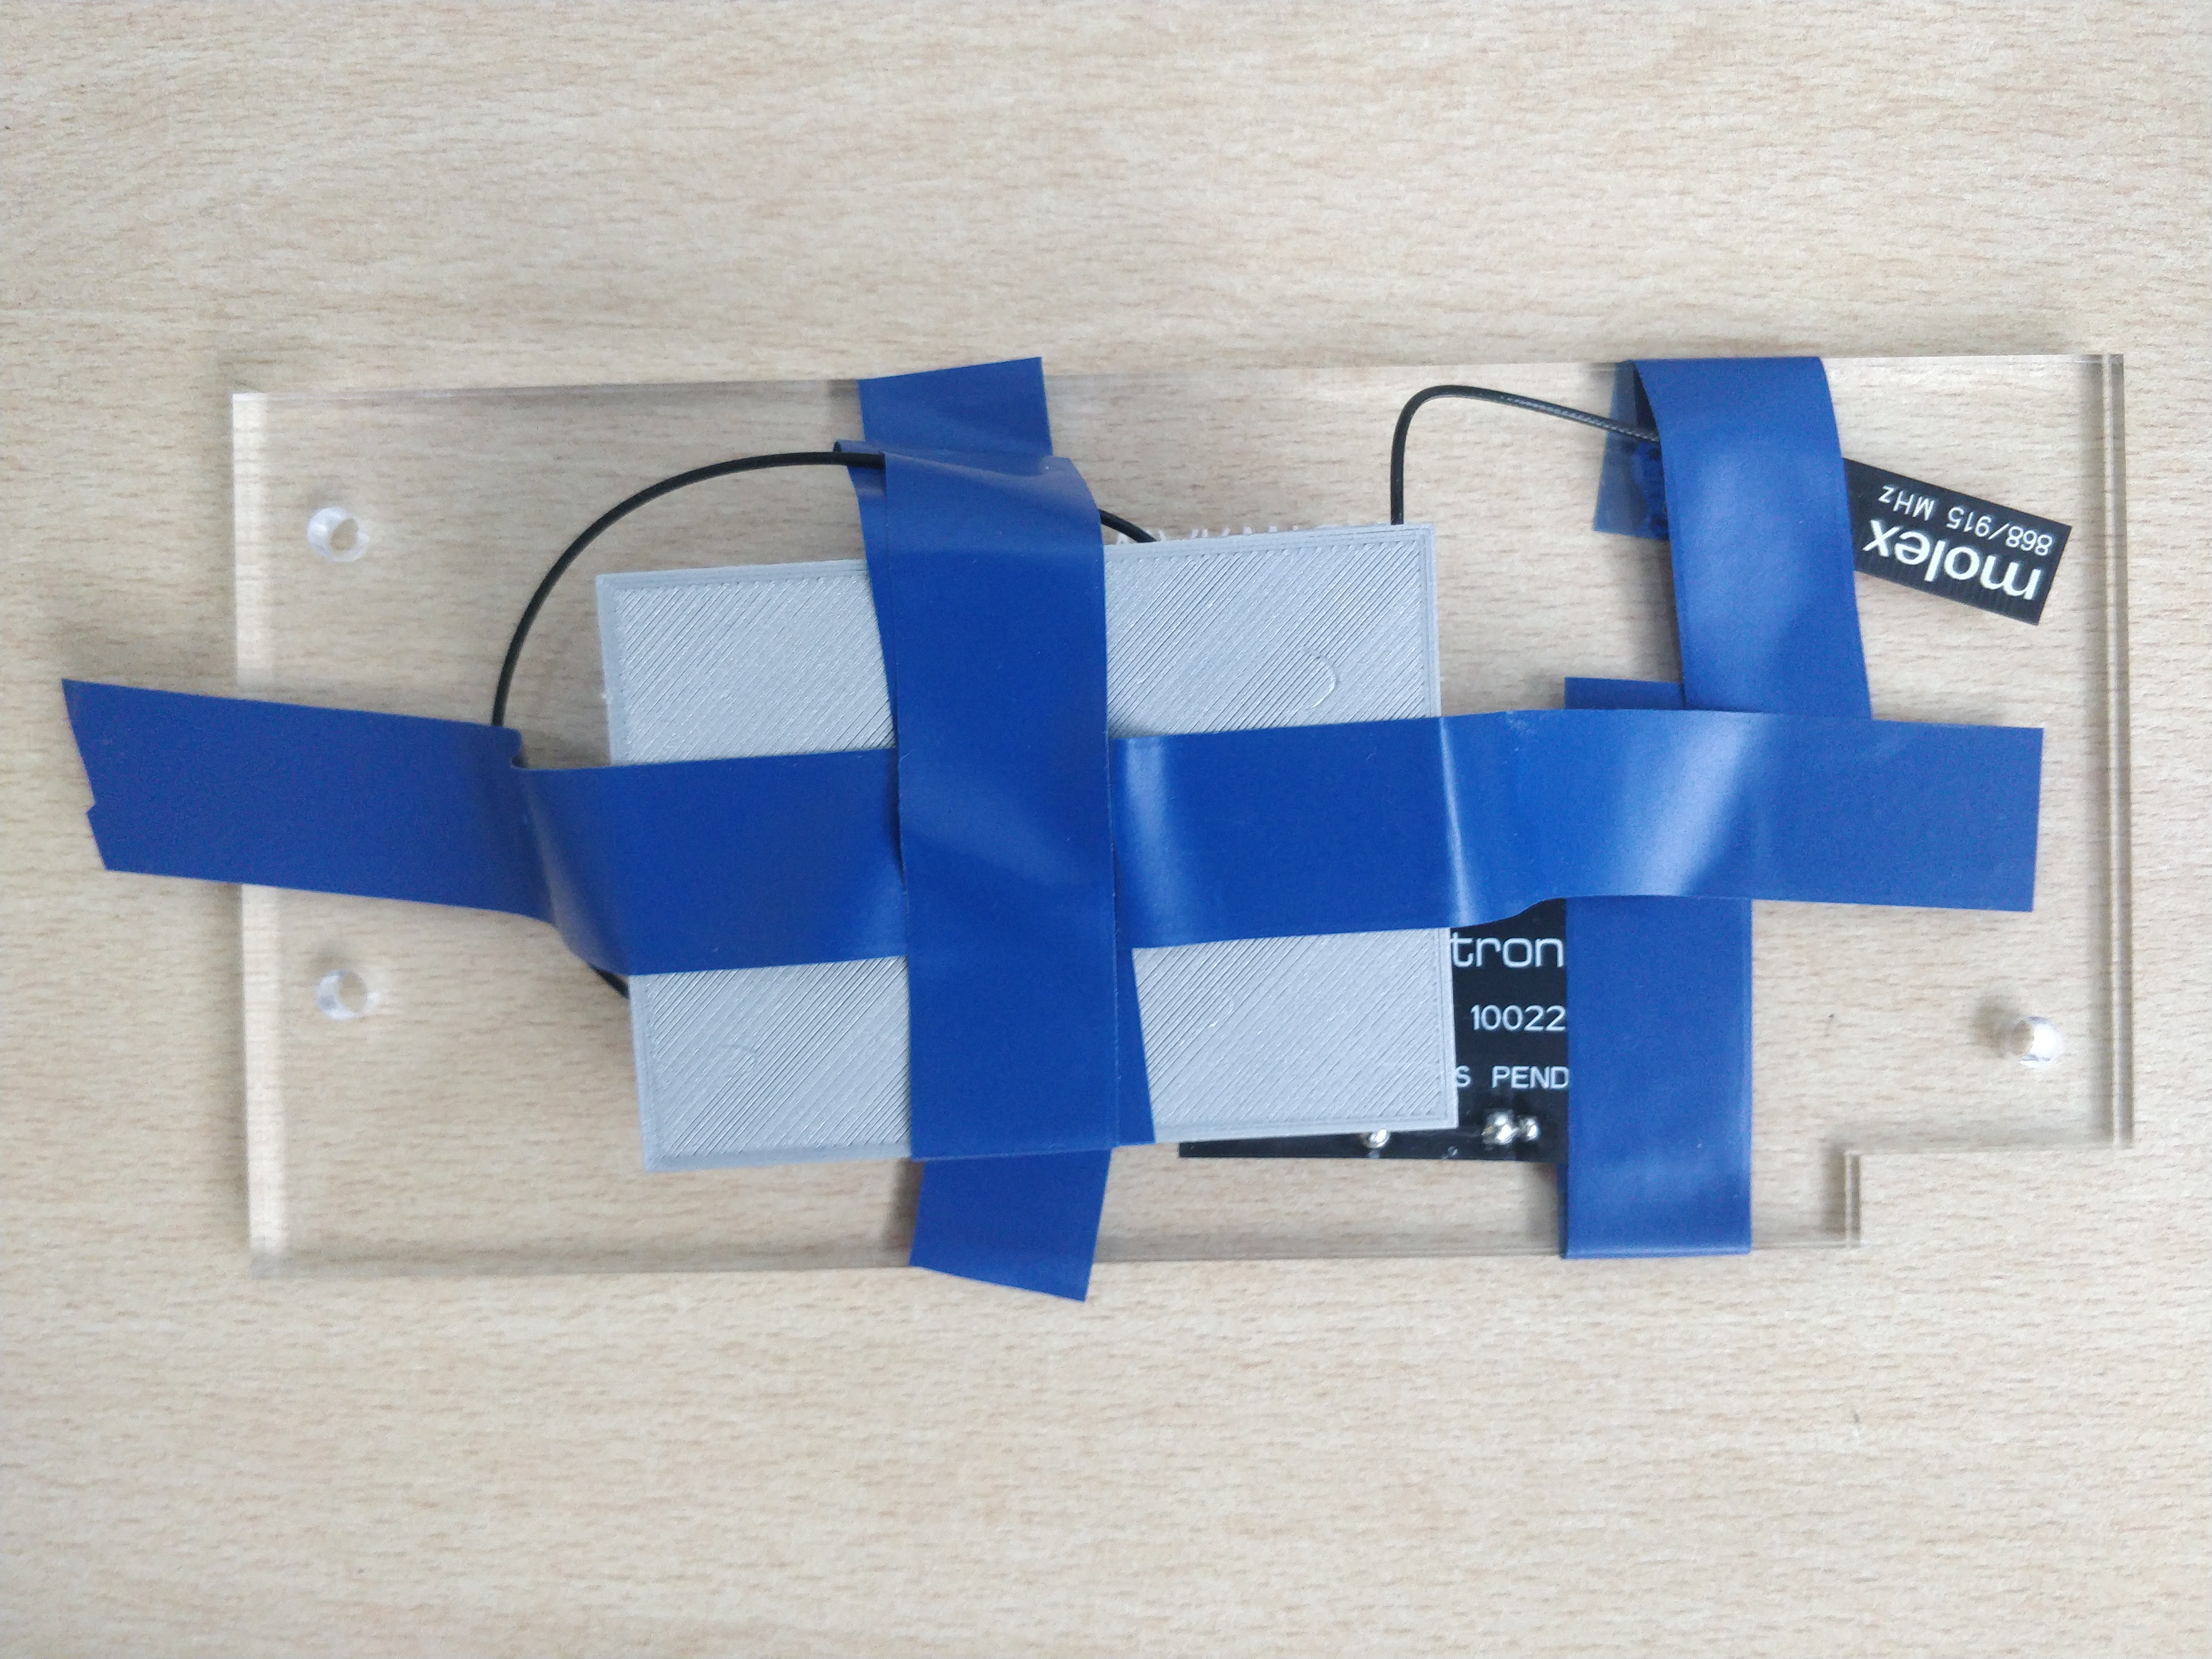
\includegraphics[height=5cm,width=\textwidth,keepaspectratio]{../figures/Pics/distancerig1.jpg}
        \caption{Overview}
    \end{subfigure}
    \hfill
    \begin{subfigure}[b]{0.475\textwidth}
        \centering
        \includegraphics[height=5cm,width=\textwidth,keepaspectratio]{../figures/Pics/distancerig2.jpg}
        \caption{Angled view}
    \end{subfigure}
    \caption{Setup used for distance testing}
    \label{fig:distancerig}
\end{figure}

\paragraph{Data}

% \begin{wrapfigure}[10]{L}{0.4\textwidth}
%     \vspace{-5pt}
%     \centering
%     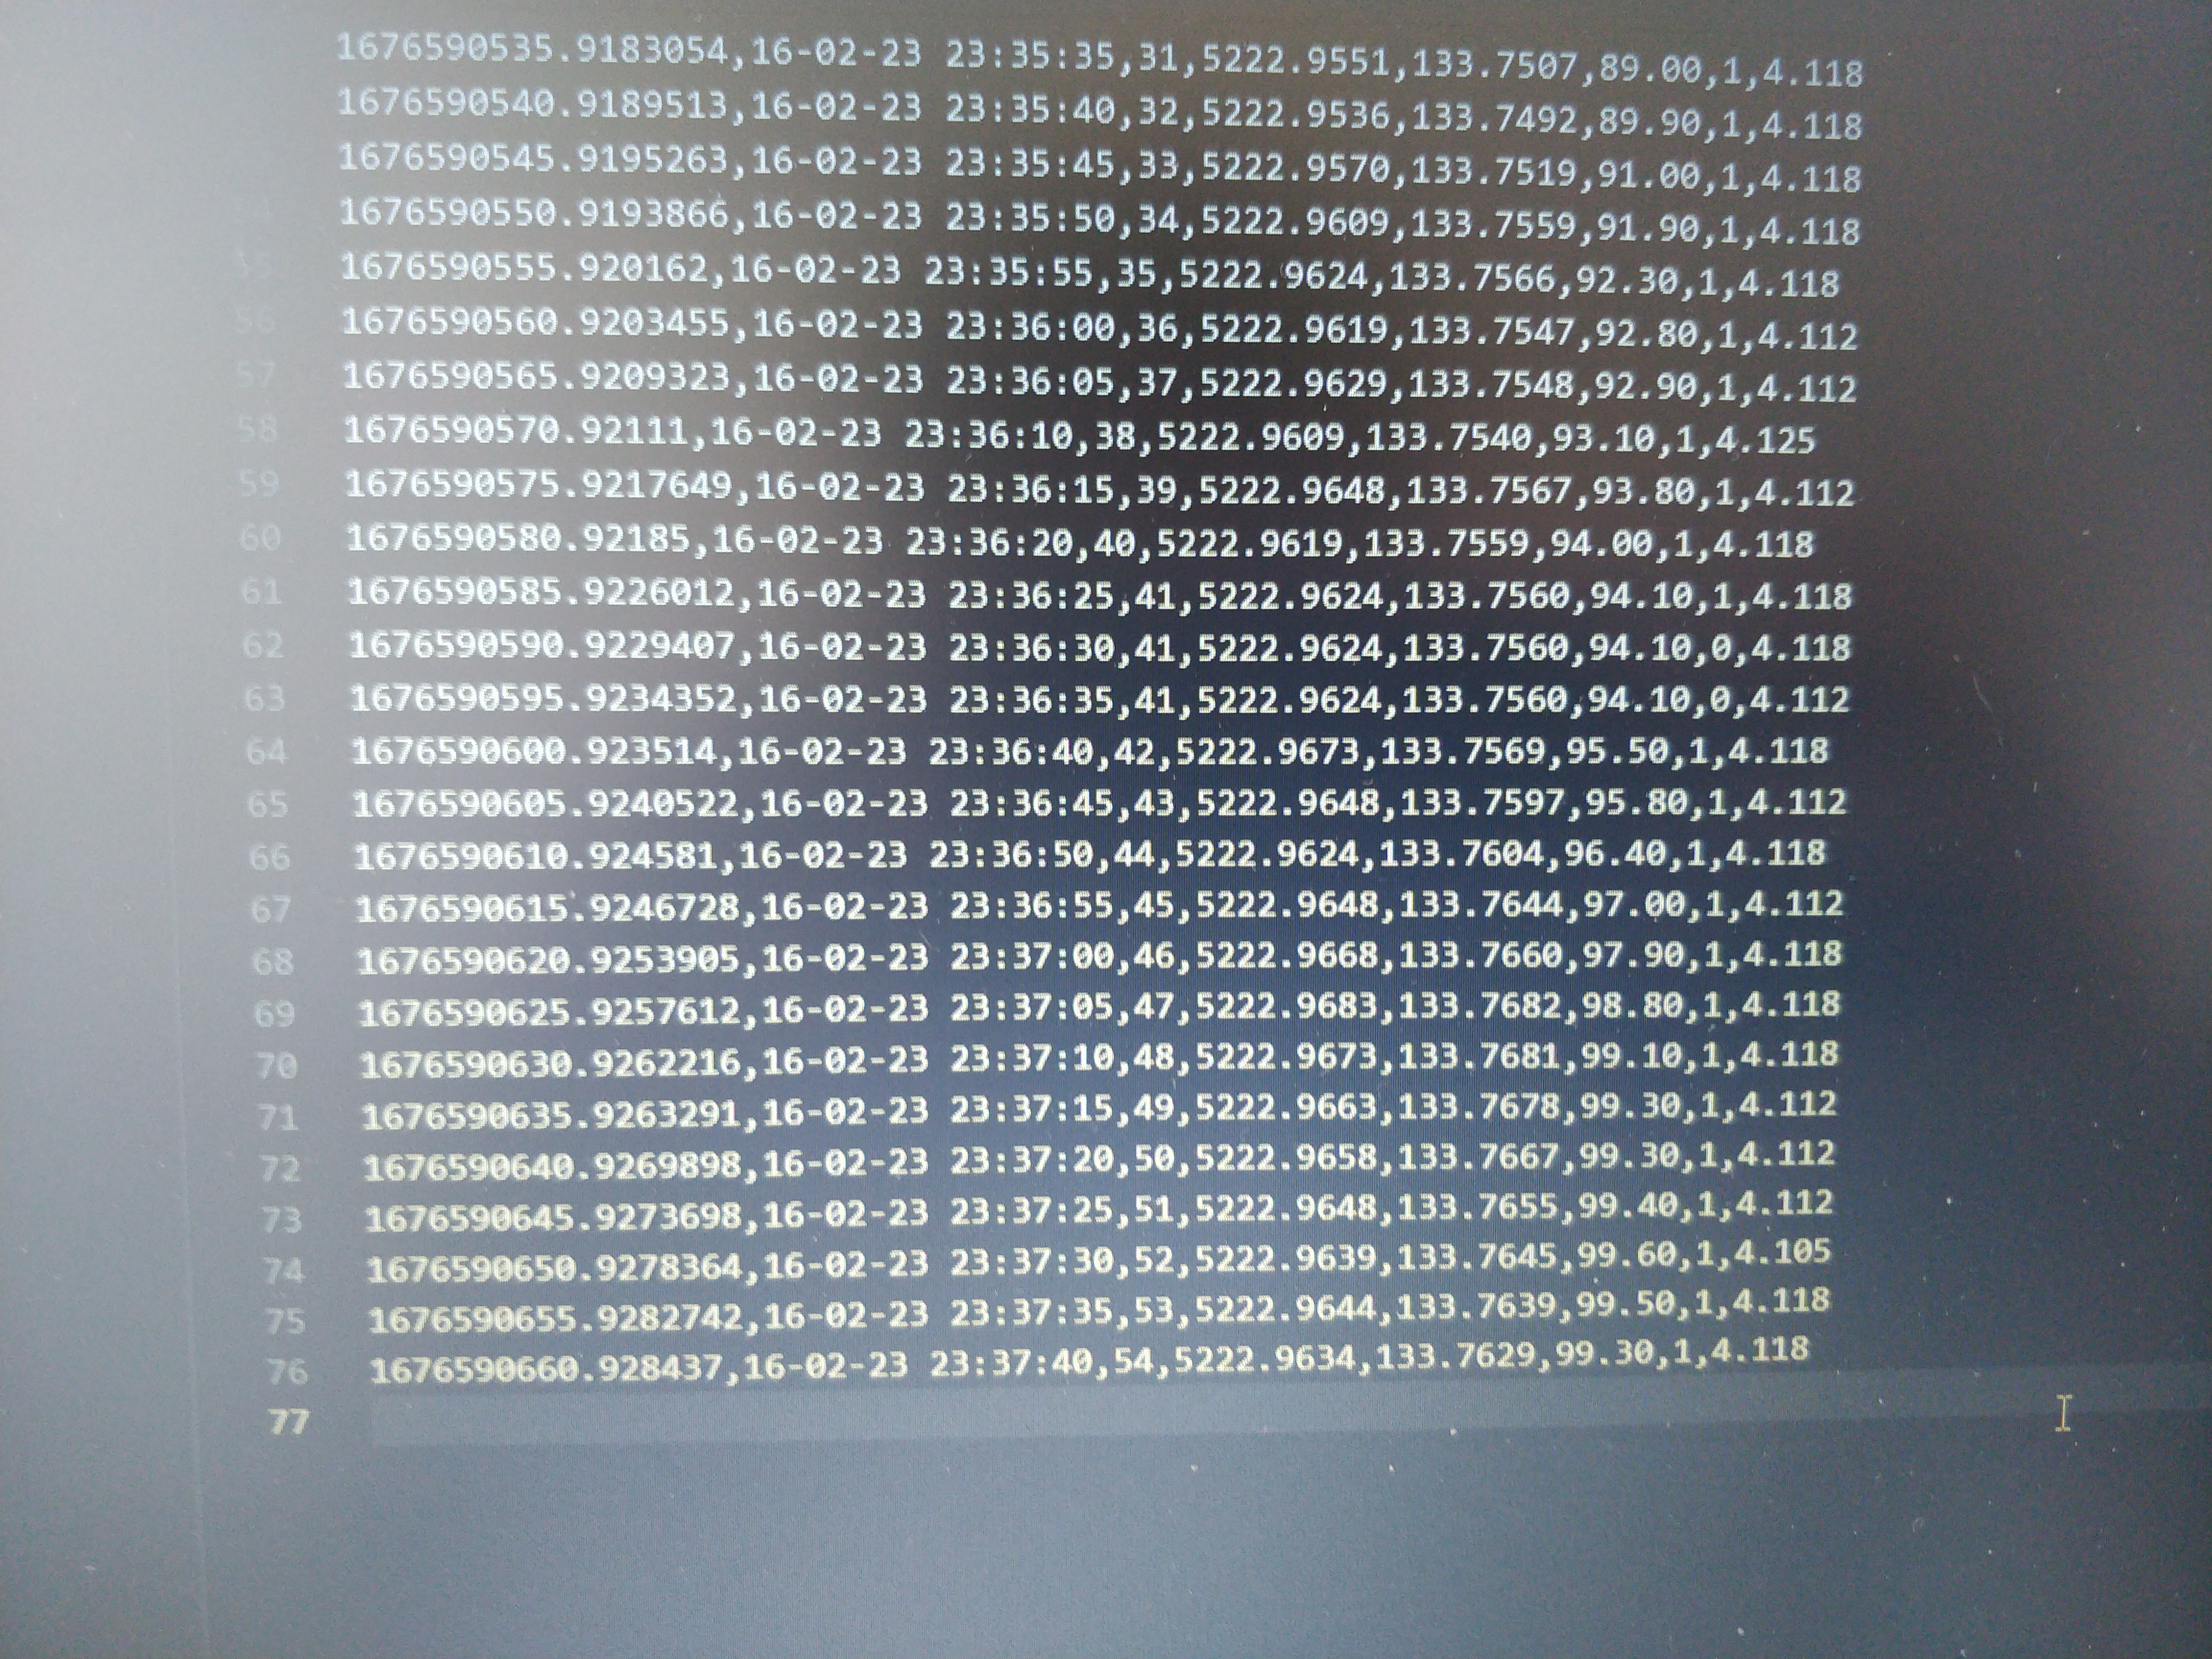
\includegraphics[width=0.4\textwidth]{../figures/Pics/distancedata.jpg}
%     \caption{Test data recordings}
%     \label{fig:distancedata}
% \end{wrapfigure}

An example of data recordings can be seen in \cref{fig:distancedata}. As mentioned previously\footnote{
    \Cref{sec:devgps}.
},
the output data is in a non-standard format, an example of which is given in \cref{table:invalidformat}.
In order for this data to be plotted, it needs to be converted into a standardised format, as per \cref{table:validformat}.

\begin{figure}[H]
    \centering
    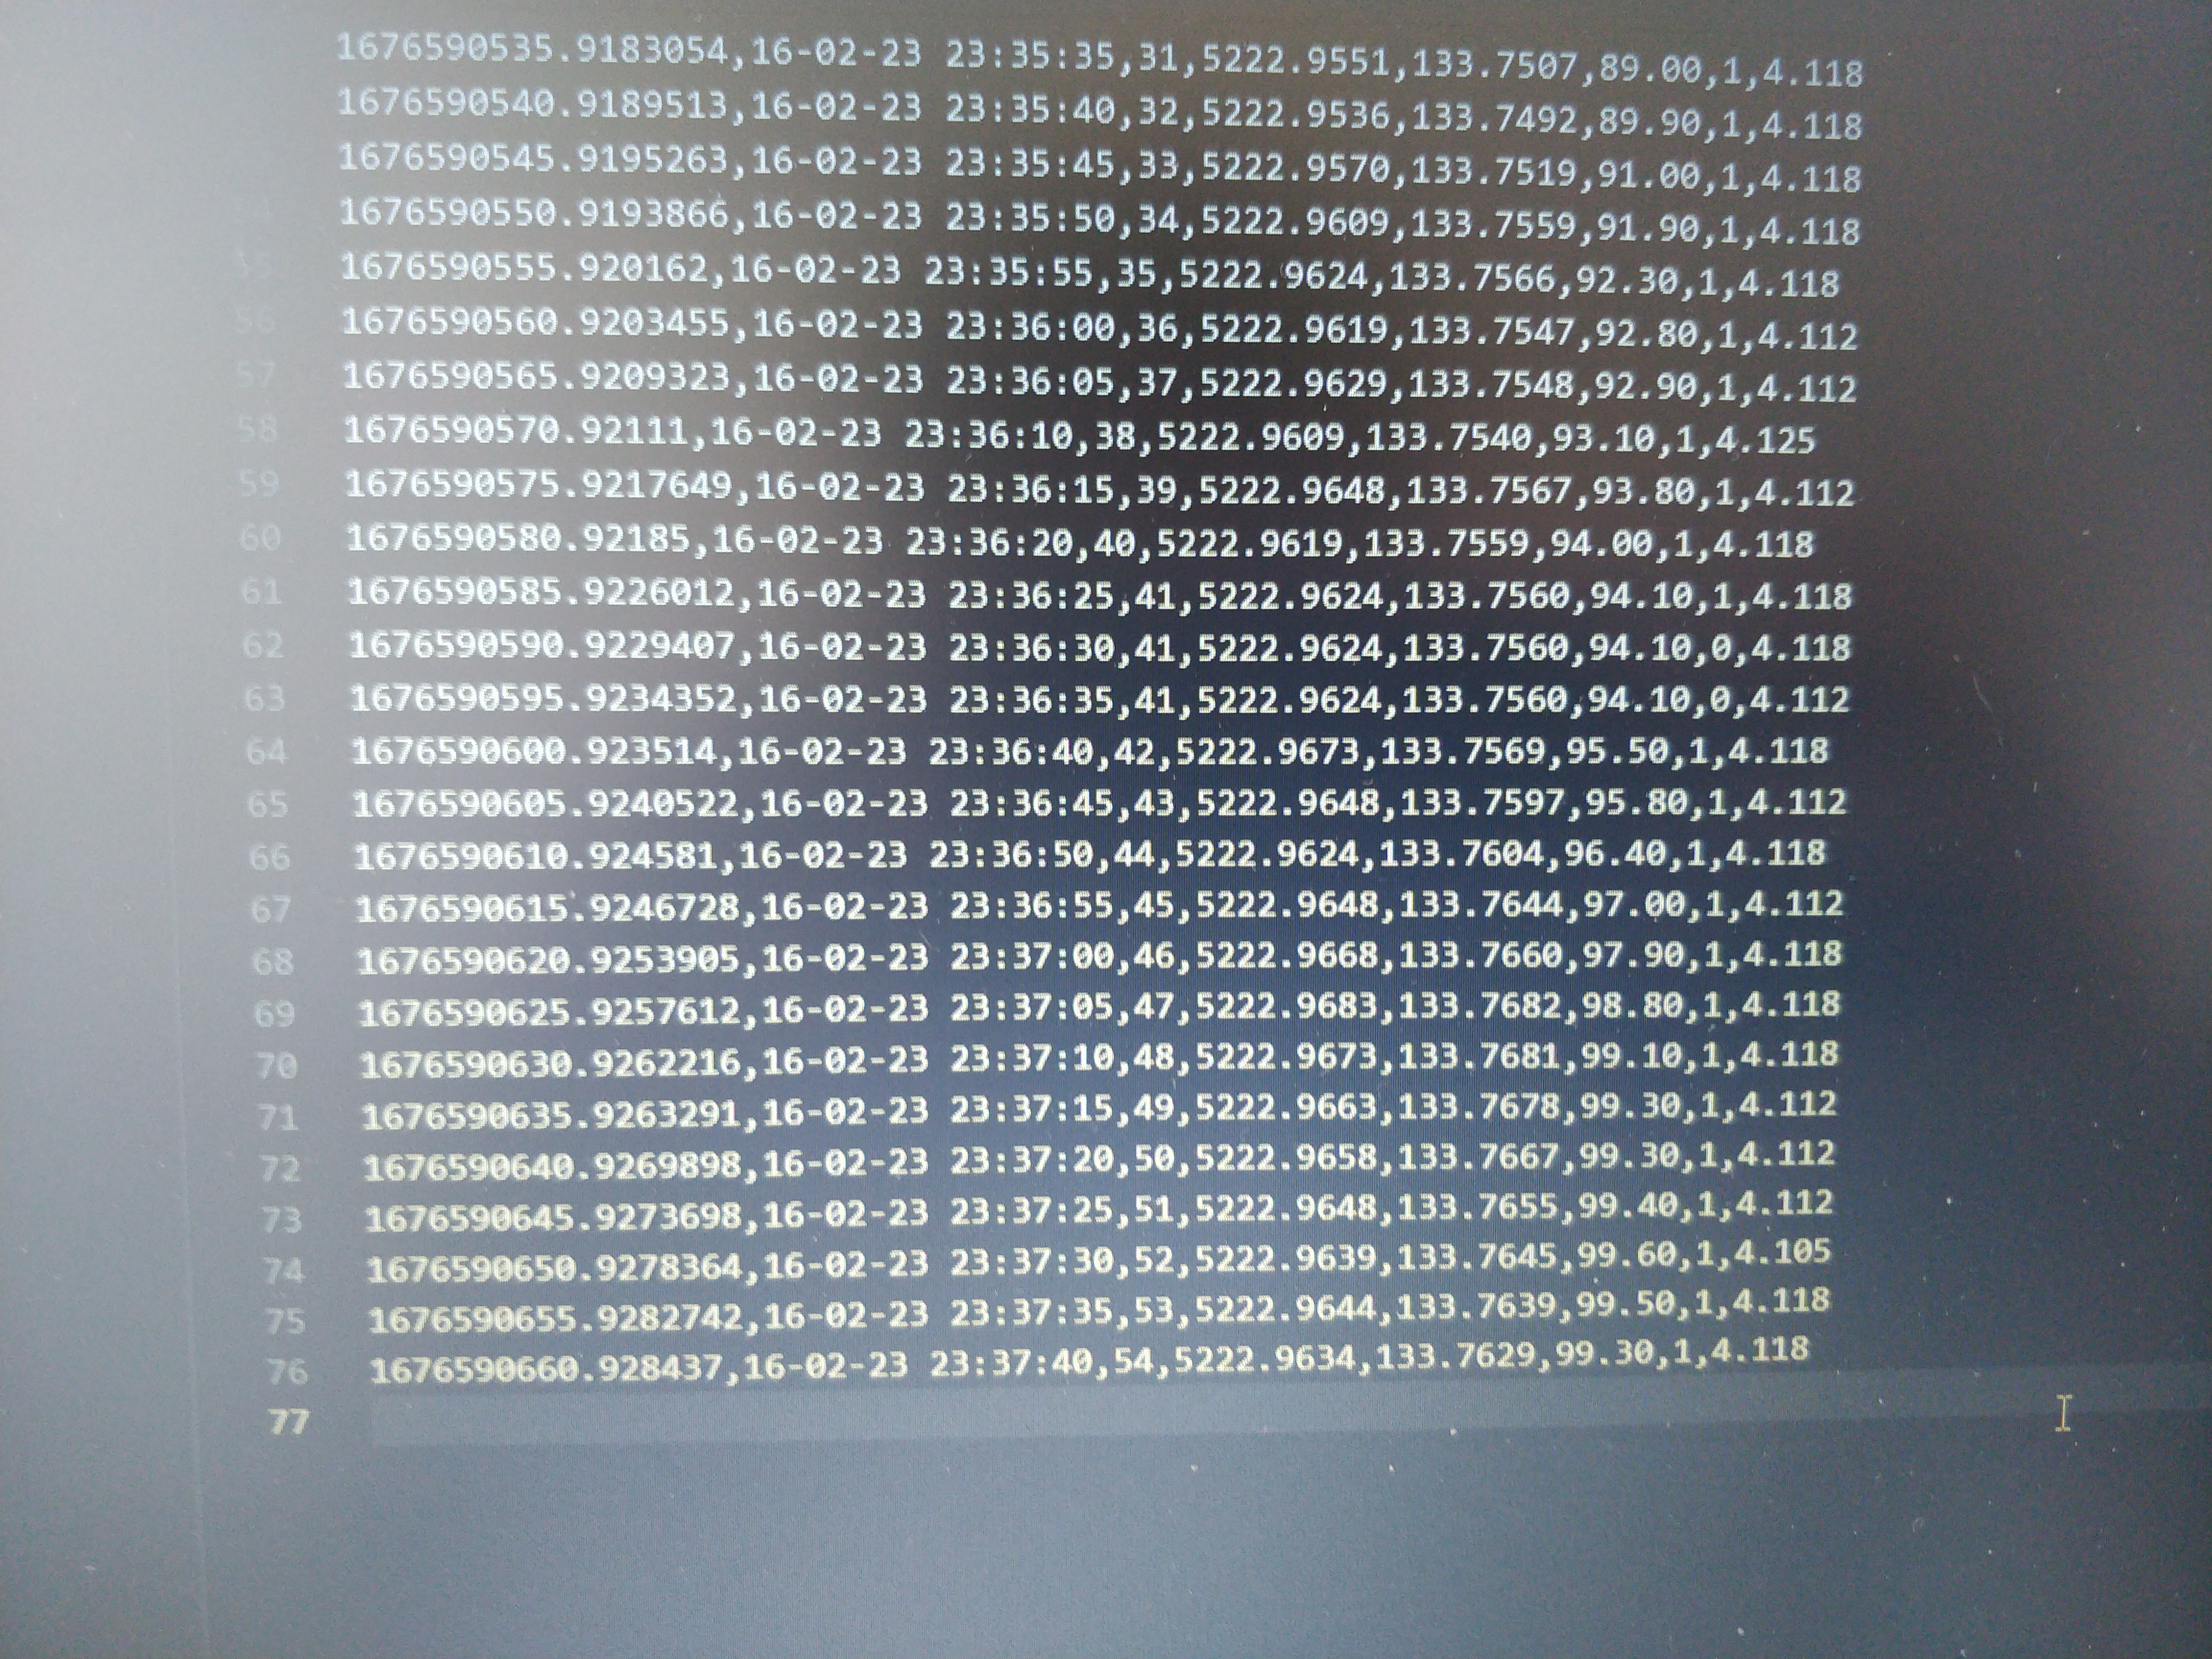
\includegraphics[width=0.7\textwidth]{../figures/Pics/distancedata.jpg}
    \caption{Test data recordings}
    \label{fig:distancedata}
\end{figure}

The first step is to add direction indicators. This supports portability, but in this case will
simply be used to determine whether the direction is positive (North or East) or negative (South or West).
While the \acrshort{gps} library is able to provide directional information \cite{adafruit:gpslibrary}, 
in this instance, the output files were simply modified to include a column of the direction, 
since only locations North and West
were recorded for any tests. The modified columns in \cref{table:invalidformat} are highlighted in blue.

\parbox{.6\linewidth}{
    \begin{xltabular}{\linewidth}{|l >{\columncolor{tableh2}}cl>{\columncolor{tableh2}}c|}
        \hline
        Latitude & Direction & Longitude & Direction \\
        \hline
        5222.9409 &	N &	133.7407 &	W \\
        5222.9409 & N &	133.7407 &	W \\
        5222.9409 &	N &	133.7404 &	W \\
        \hline
        \caption[Non-standard location data format]{Non-standard location data format, with manually added columns highlighted}\label{table:invalidformat}
    \end{xltabular}
}
\quad
\parbox{.35\linewidth}{
    \begin{xltabular}{\linewidth}{|ll|}
        \hline
        Latitude & Longitude \\
        \hline
        52'22.958  &	-1'33.76  \\
        52'22.959  &	-1'33.7594 \\
        52'22.9565 &	-1'33.7566  \\
        \hline
        \caption{Desired location data format}\label{table:validformat}
    \end{xltabular}
}

With sufficient information for processing, a script was then written to convert the given format into standardised
degrees-minutes format, as per \cref{table:validformat}, the code for which can be found in \cref{script:locationformatconverter}.
The script works by processing the location columns of each
row. It performs a regular expression match to extract the minutes from the degrees, and return both in an array [lines 6-7].
It then determines the polarity by the relevant direction column, and adds the degree separator (\textquotesingle) as necessary [lines 12-14].
Finally, it writes the new format data to a new file, which can then be used for plotting.


\paragraph{Plotting}
The plotting software of choice was QGIS, a free and open-source \acrshort{gis} software package.
While QGIS has many advanced features, one of the most useful in this case is the ability to lay \acrshort{gps}
coordinates over a map. It furthermore accepts many formats of location data, including \gls{kml} markup,
which will be important as part of the verification step.

\subsubsection{Test specification}
Due to blind recording, the test is carried out with no knowledge as to how successful it is.
The transmitter was powered on by connecting the battery, and the script on the receiver\footnote{
    \Cref{pi:battery}.
} was started. The tracker was then carried around the predetermined route. At the same time,
an app based \acrshort{gps} tracker was started, which records location data independently.
When the route was complete, the data was downloaded for later processing and comparison
to the externally recorded data.

\paragraph{Risks}
Inclement weather may cause a problem for the circuitry, as the casing is not 
waterproofed. 
Otherwise, only typical precautions when travelling outdoors near roads are 
necessary. 

\subsubsection{Test one}
The route was determined to include walking behind the School of Engineering and around
Lord Bhattacharyya Way while holder the transmitter.
This route covered a maximum straight line distance of \qty{175}{\m}
and involved parts with direct line of sight to the receiver, and large sources of interference
in other areas (e.g. buildings, antennae, girders, etc).

This test was performed with perhaps what could be considered the worst possible conditions,
and success from hereupon would determine whether an altered setup was required. To check suitability,
after the test was run, the data logs would be checked to see whether there was consistent location
information. If so, a second test at a greater distance would be performed. If not, the
setup would be revisited.

\paragraph{Results}
After the test was performed, the logs appeared to indicate successful transmission, although
this could not be analysed at the time. As such, a second test at a much greater distance was
performed immediately afterwards.

\Cref{fig:dtest1} shows the recorded points in red\footnote{
    Data sample in \cref{table:distancetest1}.
} and the externally recorded route in blue\footnote{
    Data sample in \cref{kmltest1}.
}
after processing. As can be seen, the results are well-matched. Despite the extremely poor
testing conditions, the tracker operated surprisingly well.

\begin{figure}[htbp]
    \centering
    \includegraphics[height=10cm]{../figures/maps/test1 overlay.png}
    \caption[Distance test one overlay]{Location recordings with route overlay}
    \label{fig:dtest1}
\end{figure}

% \begin{wrapfigure}{R}{0.7\textwidth}
%     \vspace{-5pt}
%     \centering
%     \includegraphics[width=0.65\textwidth]{../figures/maps/test1 overlay.png}
%     \caption[Distance test one overlay]{Location recordings with route overlay}
%     \label{fig:dtest1}
% \end{wrapfigure}

A cluster of points next
to Physical Sciences, is likely points recorded in A3.27, but offset due to inaccuracies
in location while indoors. A smaller cluster next to Car Park 10 is due to a slightly longer
period of time spent in that location.

There are no noticeable errors or omissions present. The location data recorded by the
tracker also appears to be more accurate to the precise route followed than is indicated by
app-based tracker.

\subsubsection{Test two}
Given the apparent positive results of the first test, the second test 
was devised to cover a much greater distance. In this case, the route consisted 
of Kirby Corner Rd. and Charter Ave. in a large triangle, with the greatest distance 
\qty{1.2}{\km} away. This test was devised in this manner to cover the most extreme 
capabilities of the tracker, since it is impossible to determine live whether a 
range is too great. 

The route includes a number of points that would be in `line of sight' (were it not for foliage),
in addition to areas of dense foliage and building obstructions. 

Due to the distances involved, the mode of transportation chosen was bicycle. This would 
at least affect the distance between reported locations. It is also possible that 
transmissions would be affected due to the speed. Furthermore, the tracker could no longer
be held and would have to be carried in a pocket, which may affect transmission capabilities. 

\paragraph{Results}
After testing, the logs appeared to have much fewer records than expected\footnote{
    Data sample in \cref{table:distancetest2}.
}. Furthermore, the 
app-based tracker failed to work. In \cref{fig:dtest2}, the travelled route was drawn on afterwards.
Noticeably, there are far fewer points plotted, and of that, the furthest was \qty{436}{\m} away with 
the majority of the route missing. 
This position did not have clear sight, however it was a position with the `least' obstruction
at that distance. The points were spaced out a greater distance,  which was expected. 

\begin{figure}[htb!]
    \centering
    \includegraphics[height=12cm]{../figures/maps/test2 overlay.png}
    \caption[Distance test two overlay]{Location recordings with route overlay}
    \label{fig:dtest2}
\end{figure}

% \begin{wrapfigure}{R}{0.7\textwidth}
%     \vspace{-5pt}
%     \centering
%     \includegraphics[width=0.65\textwidth]{../figures/maps/test2 overlay.png}
%     \caption[Distance test two overlay]{Location recordings with route overlay}
%     \label{fig:dtest2}
% \end{wrapfigure}

Focusing on the points recorded on Lord Bhattacharyya Way and Library Rd.,
assuming these points were sequential (\qty{5}{\s}) transmissions, this indicates an 
approximate travel speed of \qty{40}{\km\per\hour} to \qty{55}{\km\per\hour}. This 
is practically impossible to be the case, therefore suggesting there were either missing points
during transmission, or the recorded location is not precise enough to calculate 
the speed from (where it is `large'). 

Due to insufficient reporting, it is impossible to determine whether \acrshort{gps} location was
lost at any point. Periodic checks on the device suggest this did not happen\footnote{
    While searching for a fix, the \acrshort{gps} module will blink its \acrshort{led} every second.
    If a fix is found, this will increase to every fifteen, and can be used to easily indicate if 
    there is a fix \cite{adafruit:gps}. 
}.

\subsubsection{Comments}

Overall, the conclusion to be drawn from this suite of tests is that the tracker is very clearly 
viable for its purposes, however requires some points of refinement. 

Test one went extremely well, with no particular major issues identified. It is most useful 
in comparison to test two, where almost all the route was not sufficiently tracked. 
This difference likely comes down to two things - the distance travelled being obviously much greater, 
and the tracker being held in a pocket. 

Regarding distance, the area overlapped by both tests was reported on with acceptable clarity. 
This suggests the greatest issue was simply difficulty transmitting over range, or the increasing
number of interference sources as distance (and perhaps speed of travel) increased. 

It is particularly noteworthy that the test conditions were the poorest possible, possible aside 
from the addition of rain. The receiving antenna was placed indoors where it would preferably
be outdoors, and the tracker was held in a pocket where it would also be preferably exposed. 
The general area was heavily built with many sources of interference, inexhaustibly 
including trees, buildings, and metal structures. While elevated, the surrounding area was heavily built
up, with only a small area of space between buildings where the ground (and thereby, tracker) could be seen\footnote{
    This area is where Car Park 9 is located, however it is still has much foliage in the way. 
}.  
The location in particular, a university campus, suggests that there was also a 
higher likelihood of \acrshort{rf} interference sources.  

Finally, the data, while indicative of function, is far from complete. Performing more tests, especially in different 
conditions, to accurately determine the limits of the tracker conclusively would be advised. 
The information gleaned from these tests is meaningful, yet incomplete in thoroughness. 



   % 23 pages


\chapter{Conclusions}



\section{Assessment}
The project success will be assessed against specified the aims\footnote{
    \Cref{sec:aim}.
} and objectives\footnote{
    \Cref{sec:objectives}.
}.

\subsection{Assessment of objectives}
The objectives outline the steps of the project that needed to be followed for success.
Analysis of met objectives is available in \cref{table:objeval}, where success of a give point is
determined by whether the objective was met \fcolorbox{black}{tableg}{\rule{0pt}{5pt}\rule{5pt}{0pt}}\,, 
unmet \fcolorbox{black}{tabler}{\rule{0pt}{5pt}\rule{5pt}{0pt}}\,, 
or somewhat met \fcolorbox{black}{tablea}{\rule{0pt}{5pt}\rule{5pt}{0pt}}\,. 

{\small
\begin{xltabular}{\linewidth}{|>{\raggedright\arraybackslash}p{6cm}|>{\color{white}}Z|}
    \hline
    \rowcolor{tableh2}
    Objective & \textcolor{black}{Met?} \\
    \hline
    \endhead
    \endfoot

    \hline
    Research cat characteristics & \cellcolor{tableg} \\ \hline
    Research \gls{lora} radio requirements & \cellcolor{tableg} \\ \hline
    Design the system and specification & \cellcolor{tableg} \\ \hline
    Develop the tracker according to specification & \cellcolor{tablea}Further details can be found in \cref{table:speceval}. \\ \hline
    Perform verification tests & \cellcolor{tablea}Tests were performed, but were limited in completeness. More were required. \\ \hline
    Develop \acrshort{pcb}, fit to harness, and live-test & \cellcolor{tabler} \\ \hline
    Certification & \cellcolor{tabler} \\ \hline
    
    \caption{Objectives evaluation}\label{table:objeval}
\end{xltabular}
\vspace{-11pt}
}

Colour progression indicates that,
while the project started off well, completion began to suffer as time passed. 

\subsection{Assessment of aims and specification}

{\small
\begin{xltabular}{\linewidth}{|>{\raggedright\arraybackslash}p{4.5cm}|>{\color{white}}Z|}
    \hline
    \rowcolor{tableh2}
    Aim & \textcolor{black}{Met?} \\
    \hline
    \endhead
    \endfoot

    \rowcolor{tableh1}
    \multicolumn{2}{|c|}{Fundamentals} \\
    \hline
    Obtain \acrshort{gps} location & \cellcolor{tableg} \\ \hline
    Transmit via \gls{lora} & \cellcolor{tableg} \\ \hline
    Transmit remotely for a significant period of time & \cellcolor{tableg}Up to fifteen hours \\ \hline
    Transmit at a regular interval & \cellcolor{tableg}Every five seconds \\ \hline
    

    \rowcolor{tableh1}
    \multicolumn{2}{|c|}{Improvements} \\
    \hline
    Ergonomics & \cellcolor{tabler}The product is not designed for use with a pet \\ \hline
    Stability & \cellcolor{tablea}Only the receiver handles errors\\ \hline
    Installable & \cellcolor{tablea}No specific tools required for installation, however 
        it does not have appropriate casing to be mounted \\ \hline
    Location information easily viewable & \cellcolor{tablea}Information is viewable, but requires familiarity 
        with Bash \\ \hline
    

    \rowcolor{tableh1}
    \multicolumn{2}{|c|}{Production} \\
    \hline
    General safety and suitability & \cellcolor{tabler}No safety measures in place \\ \hline
    Resistance to damage and weather & \cellcolor{tablea}Some resistance to damage \\ \hline
    Certification requirements and law compliance & \cellcolor{tabler} \\ \hline
    Scale considerations & \cellcolor{tabler} \\ \hline
    
    \caption{Aims evaluation}\label{table:aimseval}
\end{xltabular}
\vspace{-11pt}
}

\Cref{table:aimseval} shows that the Fundamental aims have been met, and shows a 
similar colour progression to \cref{table:objeval} in that primary points were met, but 
later ones were not.
By meeting the Fundamental aims, the viability of the product has been demonstrated, 
and much from thereon is to improve and refine the design for consumer suitability.

\subsubsection{Assessment of specification}
This will provide a more granular overview of which elements of the specification
in \cref{sec:spec} were met. 

{\small
\begin{xltabular}{\linewidth}{|>{\raggedright\arraybackslash}p{4.5cm}|>{\color{white}}Z|}
    \hline
    \rowcolor{tableh2}
    Specification & \textcolor{black}{Met?} \\
    \hline
    \endhead
    \endfoot

    \rowcolor{tableh1}
    \multicolumn{2}{|c|}{Reporting} \\
    \hline
    Timing & \cellcolor{tablea}Performs better than \qty{30}{\s}, but no way 
        of minimising transmission gaps to under \qty{300}{\s} \\ \hline
    Distance & \cellcolor{tablea}Subject to more thorough testing to find the reliable limit. 
        Current data shows transmission is possible from over \qty{400}{\m}, however this is not consistent \\ \hline    

    \rowcolor{tableh1}
    \multicolumn{2}{|c|}{Portability} \\
    \hline
    Small form-factor & \cellcolor{tablea}Dimensions measure \qtyproduct{52 x 68 x 17}{\mm}\footnote{\Cref{fig:case2dwg}.} \\ \hline
    Lightweight & \cellcolor{tableg}Weight is \qty{55}{\g}, a \qty{63}{\percent} improvement\\ \hline
    Battery powered & \cellcolor{tableg}Battery life is \qty{15}{\hour}, a \qty{67}{\percent} improvement \\ \hline
    Attachable & \cellcolor{tabler} \\ \hline    

    \rowcolor{tableh1}
    \multicolumn{2}{|c|}{Suitability} \\
    \hline
    Installable & \cellcolor{tabler} \\ \hline
    Compliance & \cellcolor{tabler}  \\ \hline

    \rowcolor{tableh1}
    \multicolumn{2}{|c|}{Reliability} \\
    \hline
    Stable & \cellcolor{tablea}Fault handling in receiver code \\ \hline
    Fault resistant & \cellcolor{tablea}Some shock resistance in the casing \\ \hline
    Repairable & \cellcolor{tableg}No proprietary parts or complex tools are used,
         however technical knowledge is required \\ \hline
    Safety & \cellcolor{tabler} \\ \hline
    Deduplication & \cellcolor{tabler} \\ \hline
    
    \caption{Specification evaluation}\label{table:speceval}
\end{xltabular}
\vspace{-11pt}
}

The greater detailed view in \cref{table:speceval} indicates some points met in the aim may 
not quite meet the specification, with many such reasons overlapping.

\section{Improvements}
Using this project's findings as a basis, there are many points of 
specific improvements that can be explored in future projects. 
These will be broken down into two types: improvements that resolve an
issue that was faced during the project, and improvements that
will increase the quality of the product.

\subsection{Issue resolvers}
\paragraph{Battery connection}
There was no way to control the power to the transmitter. As soon as the
battery was connected, it would begin to transmit, and more crucially, drain
the battery. Repeated disconnections of the power port led to the
cables exposing and almost shorting at one point.
This was resolved using insulting tape\footnote{
    The taping can be seen in \cref{fig:case1img}.
}, however such a
method is only a temporary measure.

A better way of managing this
would be to use a switch across one of the battery lines,
allowing power to be killed gracefully. This has a drawback
itself in that it would require the user to power on the device
in order to recharge the battery.
A smarter, user-friendly approach would require discrete charging
circuitry to handle charging and power, which is moving towards
bespoke circuit design and out of the scope of this project. However,
this would be vital towards making this a viable consumer product.

\paragraph{Transmission errors}
Transmission errors only appeared to occur while the system was
used on a close-range basis. However, it is entirely possible for
such errors to occur on a general basis. To minimise this,
a \acrshort{crc} may be used. Another method of transmission error handling
would be to utilise \acrshort{fec} (for example, parity checks),
however this may greatly increase
the complexity of the project, and likely is not necessary given the
frequency rate of errors, packet size, and hardware capabilities.
The Radiohead library supports client-server acknowledgement
with the \lstinline{RHReliableDatagram} class, which allows
checking that a packet has been received correctly, and if not, retransmit.
This can be additionally used to notify when the tracker is no longer
able to transmit to the server (as it would fail to acknowledge the
server's checks). 

The \lstinline{RHDatagram} superclass additionally allows for addressing, meaning 
nodes (receivers) are numbered with an address 0 to 255 and only packets 
addressed to that specific node are accepted, thereby filtering out packets from 
`other' transmitters. This meets the deduplication specification point\footnote{
    \Cref{sec:dedupe}.
}, however suffers the obvious drawback of being limited by address pool. 
An alternative method would be to encode addresses into the packet information manually
rather than relying on a provided class, thereby allowing the address pool criteria 
to be virtually any size. Whatever method is chosen, the transmitters will 
also be able to encode a unique address, allowing an owner to track multiple pets. 

\paragraph{Charging time}
While the transmitter may boast an impressive battery life, the charging
time leaves much to be desired. Protocols like Qualcomm's Quick Charge
may mitigate this, however it is limited to Qualcomm \acrshortpl{soc}.
This works by negotiating a higher current over the \acrshort{usb} connection,
as the default is limited to \qty{500}{\mAh} \cite{axelson:usb}.

\subsection{Quality improvements}
\paragraph{Display}
The Pi \gls{lora} bonnet comes with an \acrshort{oled} display that
was completely unutilised. This could be used to display warnings to the user
to indicate when \acrshort{gps} is lost or the battery levels are low.

\paragraph{Advanced power management}
The Feather M0 supports underclocking, meaning that battery life
could be greatly improved. The \gls{lora} modem also supports commands
to sleep, as otherwise it stays in a passive `listening' mode that draws
some power (around \qty{2}{\mA} \cite{adafruit:loram0}).
Since it is only required to transmit, the radio can be
turned off to save power in the meantime.

\section{Additional remarks}
Some aspects have not been discussed in any great detail. 
Here, such aspects will be focused upon.

\paragraph{Environmental impact}
The project does not have an explicit environmental impact.
Manufacture of electronics in general is an environmental burden, 
as is safe disposal, and this project certainly falls within the purview
of such elements. Such considerations will be vital should this 
project be taken to manufacture, as safe disposal of electronics
and batteries in particular will be necessary. 

\paragraph{Cost} 
The overall cost of the project is not entirely straightforward 
due to the scattered and chaotic nature of the ordering.
All parts used in the project ordered through 
approved vendors totals to £198.11\footnote{
    Before \acrshort{vat}.
}. This cost does not include some components used (i.e. 
the overall cost of the project is greater), the most 
significant of which is the Pi 3. While this retails for 
£40\footnote{
    Available at 
    \href{https://thepihut.com/products/raspberry-pi-3-model-b?src=raspberrypi}{The PiHut \faExternalLink}
}, it was often seen listed on Amazon or eBay 
with a markup over \qty{120}{\%}.


\section{Evaluation}
The project was, overall, reasonably successful. 
The fundamental aims were met, and many of the objectives outlined were 
followed through. Many of the advanced aims were not met, however. 
In retrospect, some of these were rather ambitious for the timescale 
available, however are certainly worth revisiting and exploring in 
some depth in future projects built upon this one. 

One of the key takeaways is the importance of planning around expected and unexpected issues. 
While hardware delivery delays certainly held the project up significantly, having a mitigation plan 
in place such that progress in some area, whether that be more advanced design work, or a greater 
depth of research, would have been beneficial. This also assumes that alternative hardware cannot be used
at all, whereas in many cases, it potentially may be. 

One of the greatest outcomes was the successful function of the tracker despite the tight time scales.
With a small amount of refinement weatherproofing the case, the tracker is perfectly sufficient 
for function, even if it is not at the point where it is suitable for consumer use. This project 
can be used as an excellent springboard upon which to explore building a genuinely usable product. 

\subsection{Difficulties}
The overall trend indicated by the assessments performed is that many of the early points for the project 
were met, however later and more advanced points were not. The primary limiting factor to progression 
was time constraints, with the biggest contributor being delivery delays. 
As a product development focused project, there was a limited amount of work possible 
without any hardware to develop on. When hardware did finally arrive, it was incomplete,
leading to haphazard development missing components. Delays in antennae delivery (including the 
receiver antenna in particular), shifted distance testing to the final step performed, and limited 
the possibility of additional tests. This has the knock-on effect leaving an incomplete picture 
of the true capabilities of the tracker, and also shifting every subsequent step (like \acrshort{pcb} design)
to the point where they were no longer viable to tackle

In general, development for this project moved rather quickly, with the bulk of programming to produce 
a minimum viable product complete in the span of a week. Hardware delivery issues were expected, given 
global semiconductor shortages, however the true extent of delays were not adequately accounted for and 
thus led to severe delays in the project itself. 


\subsection{Admittances}
The process of code development progressed extremely smoothly. 
Prior experience with the relevant libraries helped in this regard.
Development could have proven extremely difficult, given the 
unfavourable nature of diagnosing \acrshort{rf} issues. 
This project made use of many more scripts than anticipated, 
most of which were for data handling or graphing than direct functionality. 
The programmatic nature made this all very straightforward to design and use. 





\cleardoublepage
\newgeometry{right=2cm, left=2cm, top=2.5cm, bottom=2.5cm}
\fancyfootoffset{0pt}
% \pagestyle{headii}
\chapter{References}

\nocite{*}

% \printbibliography[heading=none]

\renewcommand*{\bibfont}{\footnotesize}

\begin{singlespace}
    
    
    \printbibliography[heading=none,category=cited]% default title for `article` class: "References"
    % \restoregeometry

% \printbibliography[title={Further Reading},notcategory=cited]

    \clearpage
\thispagestyle{plain}
\pagenumbering{gobble}
    \begin{center}
        \vspace*{1cm}

        \vfill
            
        
        % \par\noindent\rule{\textwidth}{1mm}
        \textcolor{titleblue}{\rule{\linewidth}{1mm}}\par

        \vspace{0.5cm}

        \textbf{\Huge Appendices}
        
        % \par\noindent\rule{\textwidth}{1mm}
        \textcolor{titleblue}{\rule{\linewidth}{1mm}}\par

        \vfill
                        
        \vspace{0.8cm}
            
    \end{center}
\clearpage

    \clearpage
\begin{appendices}
\pagenumbering{Roman}

\chapter{Further Reading}
\printbibliography[heading=none,notcategory=cited]

\chapter{Pinout Diagrams}

\vfill

\begin{figure}[H]
    \centering
    \includegraphics[width=0.5\textwidth]{../figures/raspberry-pi-pinout.png}
    \caption[Raspberry Pi pinout]{Raspberry Pi pinout, available at \href{https://pinout.xyz}{pinout.xyz \faExternalLink}}
    \label{fig:raspipinout}
\end{figure}

\vfill

\begin{figure}[H]
    \centering
    \includegraphics[width=\textwidth]{../figures/featherm0pinout.png}
    \caption[LoRa Feather M0 pinout]{\gls{lora} Feather M0 pinout \cite{img:m0}}
    \label{fig:m0pinout}
\end{figure}

\vfill

\begin{figure}[H]        
    \centering
    \begin{subfigure}[b]{0.35\textwidth}
        \centering
        \includegraphics[angle=90,width=\textwidth,height=6cm, keepaspectratio]{../figures/gpspins.jpg}
        \caption{GPS Featherwing pins}
        \label{fig:gpspin}
    \end{subfigure}
    \hfill
    \begin{subfigure}[b]{0.6\textwidth}  
        \centering 
        \includegraphics[height=6cm,width=\textwidth, keepaspectratio]{../figures/gpsstack.jpg}
        \caption{GPS Featherwing stacked}
        \label{fig:gpstack}
    \end{subfigure}  
    \caption[GPS Featherwing pin images]{GPS Featherwing pin images, available at \href{https://www.adafruit.com/product/3133}{Adafruit \faExternalLink}}    
    \label{fig:gpspins}     
\end{figure}

\href{https://learn.adafruit.com/adafruit-ultimate-gps-featherwing/pinouts}{GPS Featherwing pinouts reference link \faExternalLink}

\vfill

\chapter{Case design}
    
\vfill
    \begin{figure}[H]
        \caption[First case print]{First case print, showing various angles}         
        \label{fig:case1img}
        \centering
        \begin{subfigure}[b]{0.4\textwidth}
            \centering
            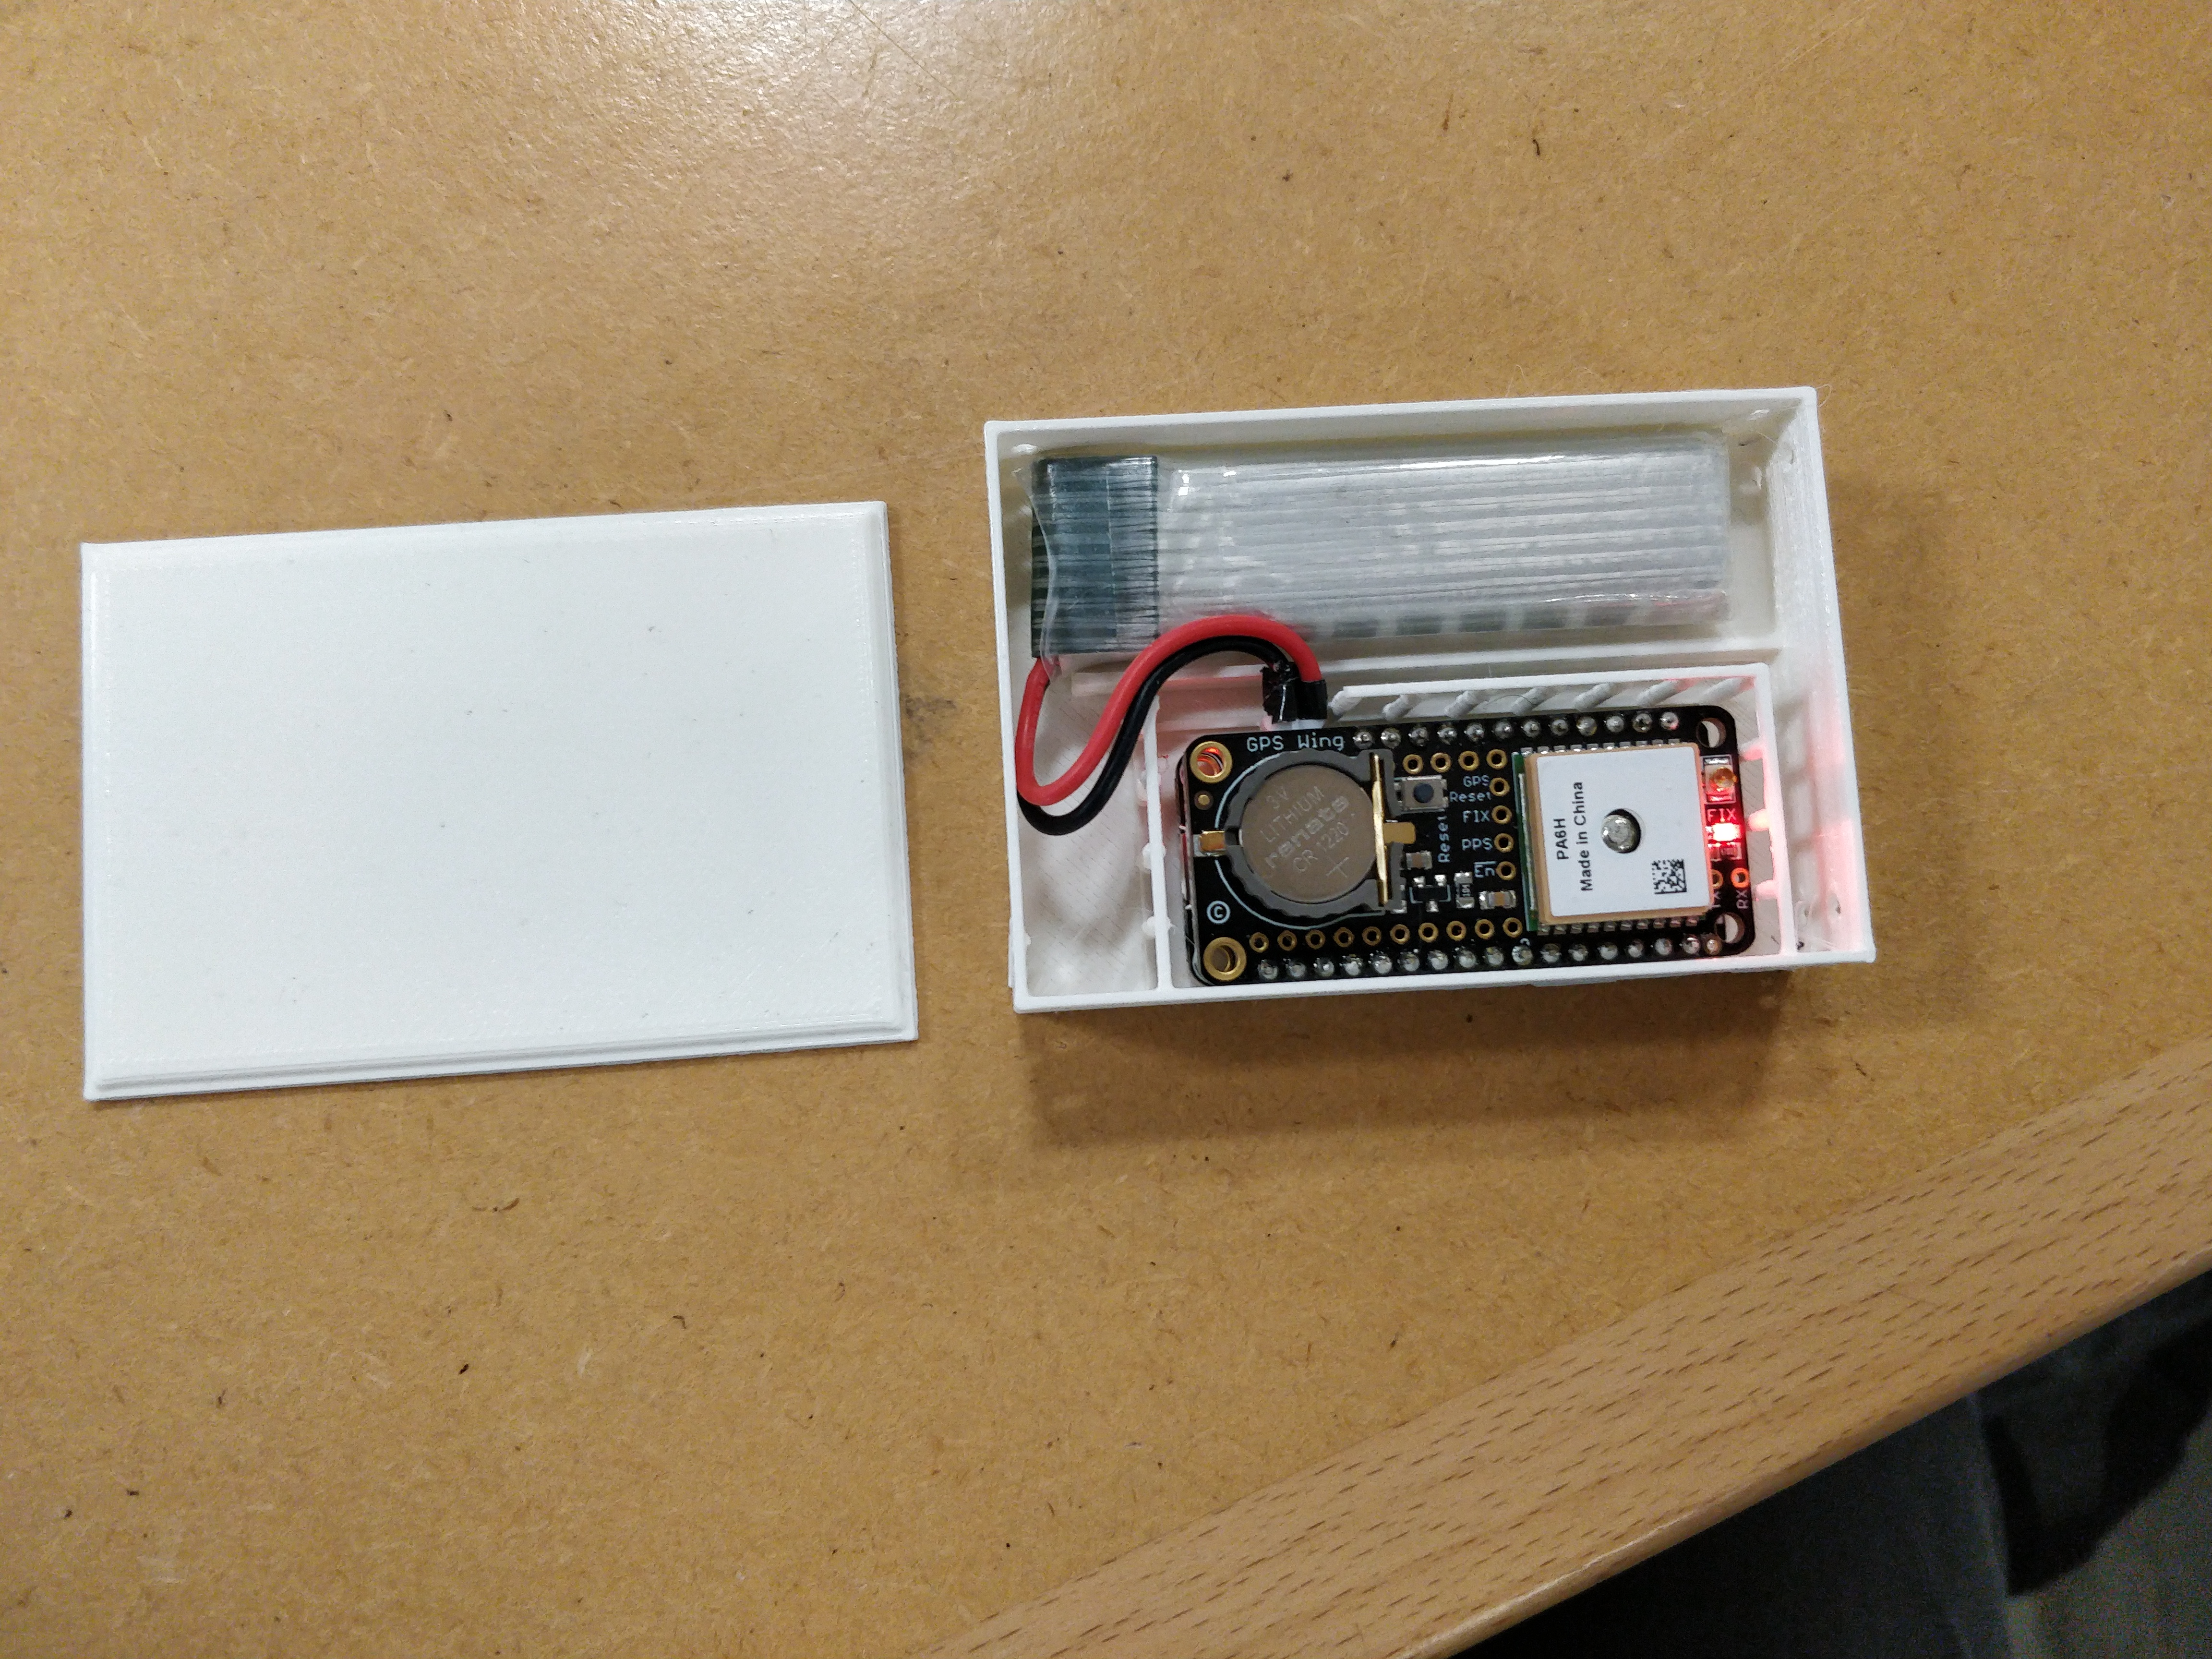
\includegraphics[angle=90,width=\textwidth]{../figures/Pics/firstcase1.jpg}
            \caption{Case overview with lid}
        \end{subfigure}
        \hfill
        \begin{subfigure}[b]{0.4\textwidth}  
            \centering 
            \includegraphics[width=\textwidth]{../figures/Pics/firstcase2.jpg}
            \caption{Battery port view}
        \end{subfigure}
        \vskip\baselineskip
        \begin{subfigure}[b]{0.4\textwidth}   
            \centering 
            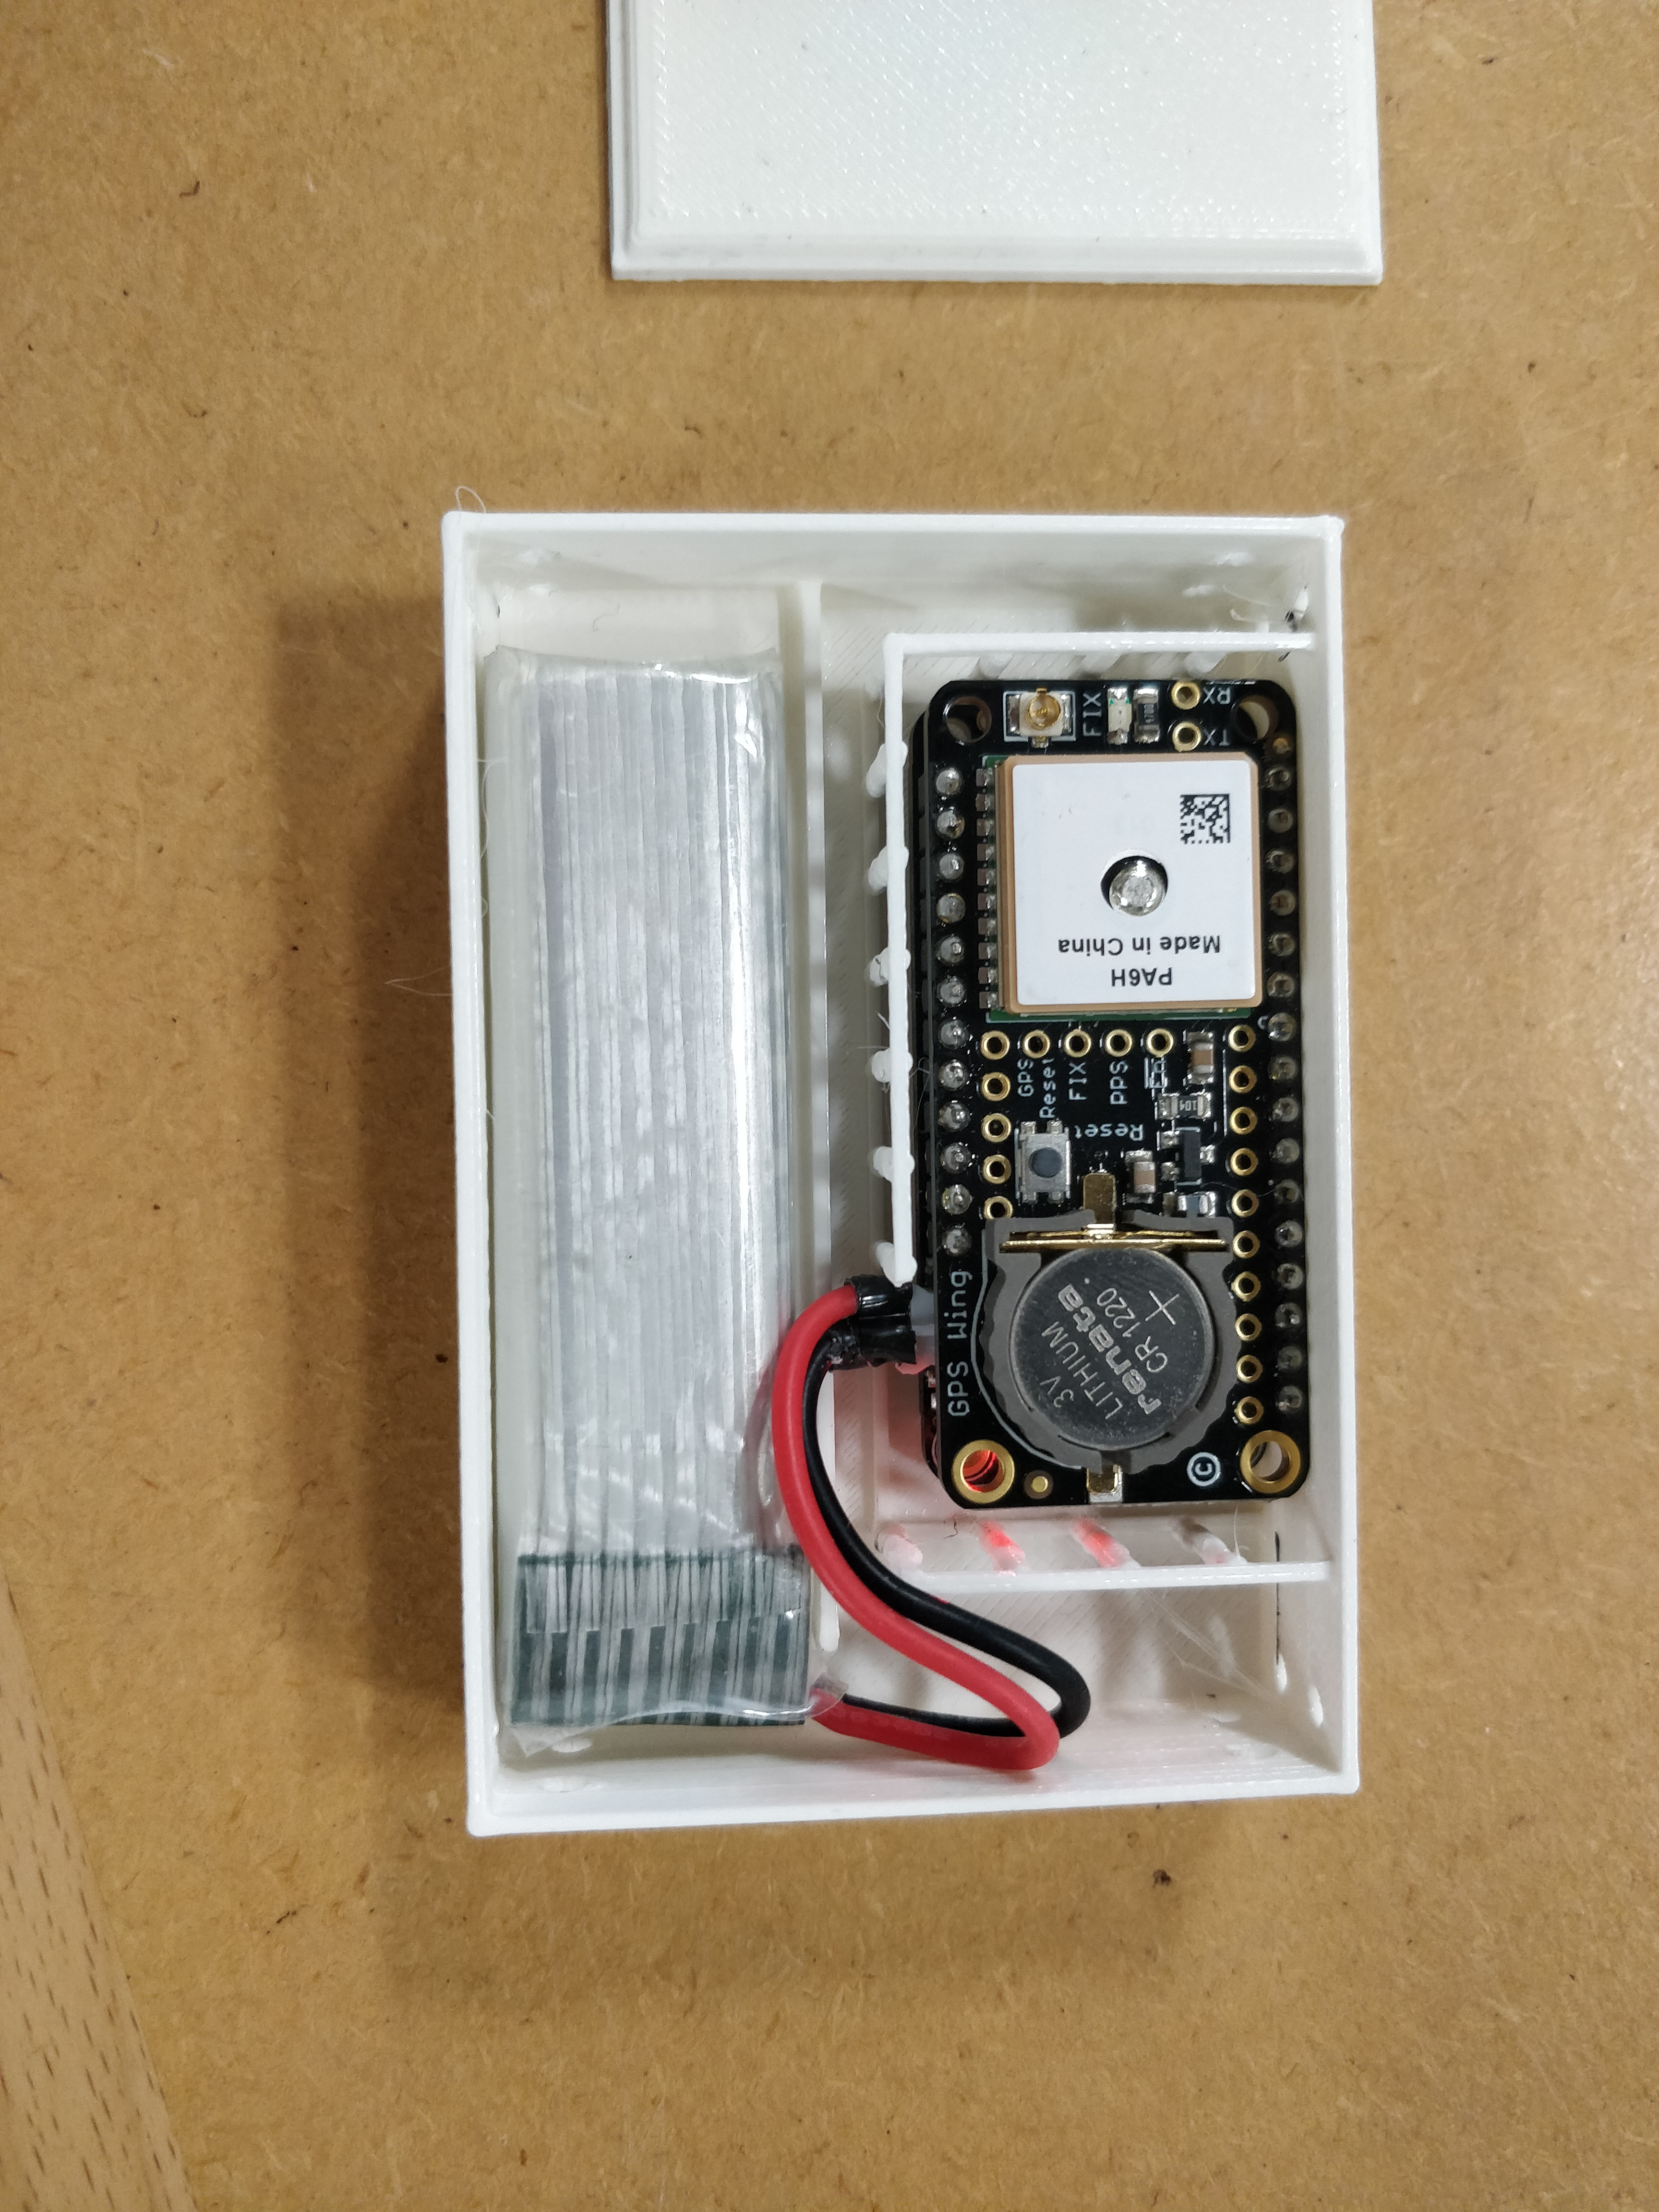
\includegraphics[width=\textwidth]{../figures/Pics/firstcase3.jpg}
            \caption{Top view}            
            \label{fig:case1top}
        \end{subfigure}
        \hfill
        \begin{subfigure}[b]{0.4\textwidth}   
            \centering 
            \includegraphics[width=\textwidth]{../figures/Pics/firstcase4.jpg}
            \caption{Angled front view}
        \end{subfigure}        
    \end{figure}
    \vfill
    \clearpage

    % \begin{figure}[H]        
    %     \label{case1dwg}
    %     \caption{Case 1 dimensional drawing}
    %     \includegraphics[angle=-90,width=\textwidth]{../../Design/case1.pdf}
    % \end{figure}  

    % \includepdf[pagecommand={},angle=-90,scale=0.9,pagecommand=\section{Case 1 dimensional drawing \label{fig:case1dwg}}]{../../Design/case1.pdf}  
    
    \begin{figure}[H]      
        \caption{Case 1 dimensional drawings}
        \includepdf[pagecommand={},angle=-90,scale=0.9]{../../Design/case1.pdf}  
        \label{fig:case1dwg}
    \end{figure}
    % \clearpage
       
    % \section{Case 2 images}
    \vfill
    \begin{figure}[H]          
        \caption[Second case print]{Second case print, showing various angles} 
        \label{fig:case2img}  
        \centering
        \begin{subfigure}[b]{0.6\textwidth}  
            \centering 
            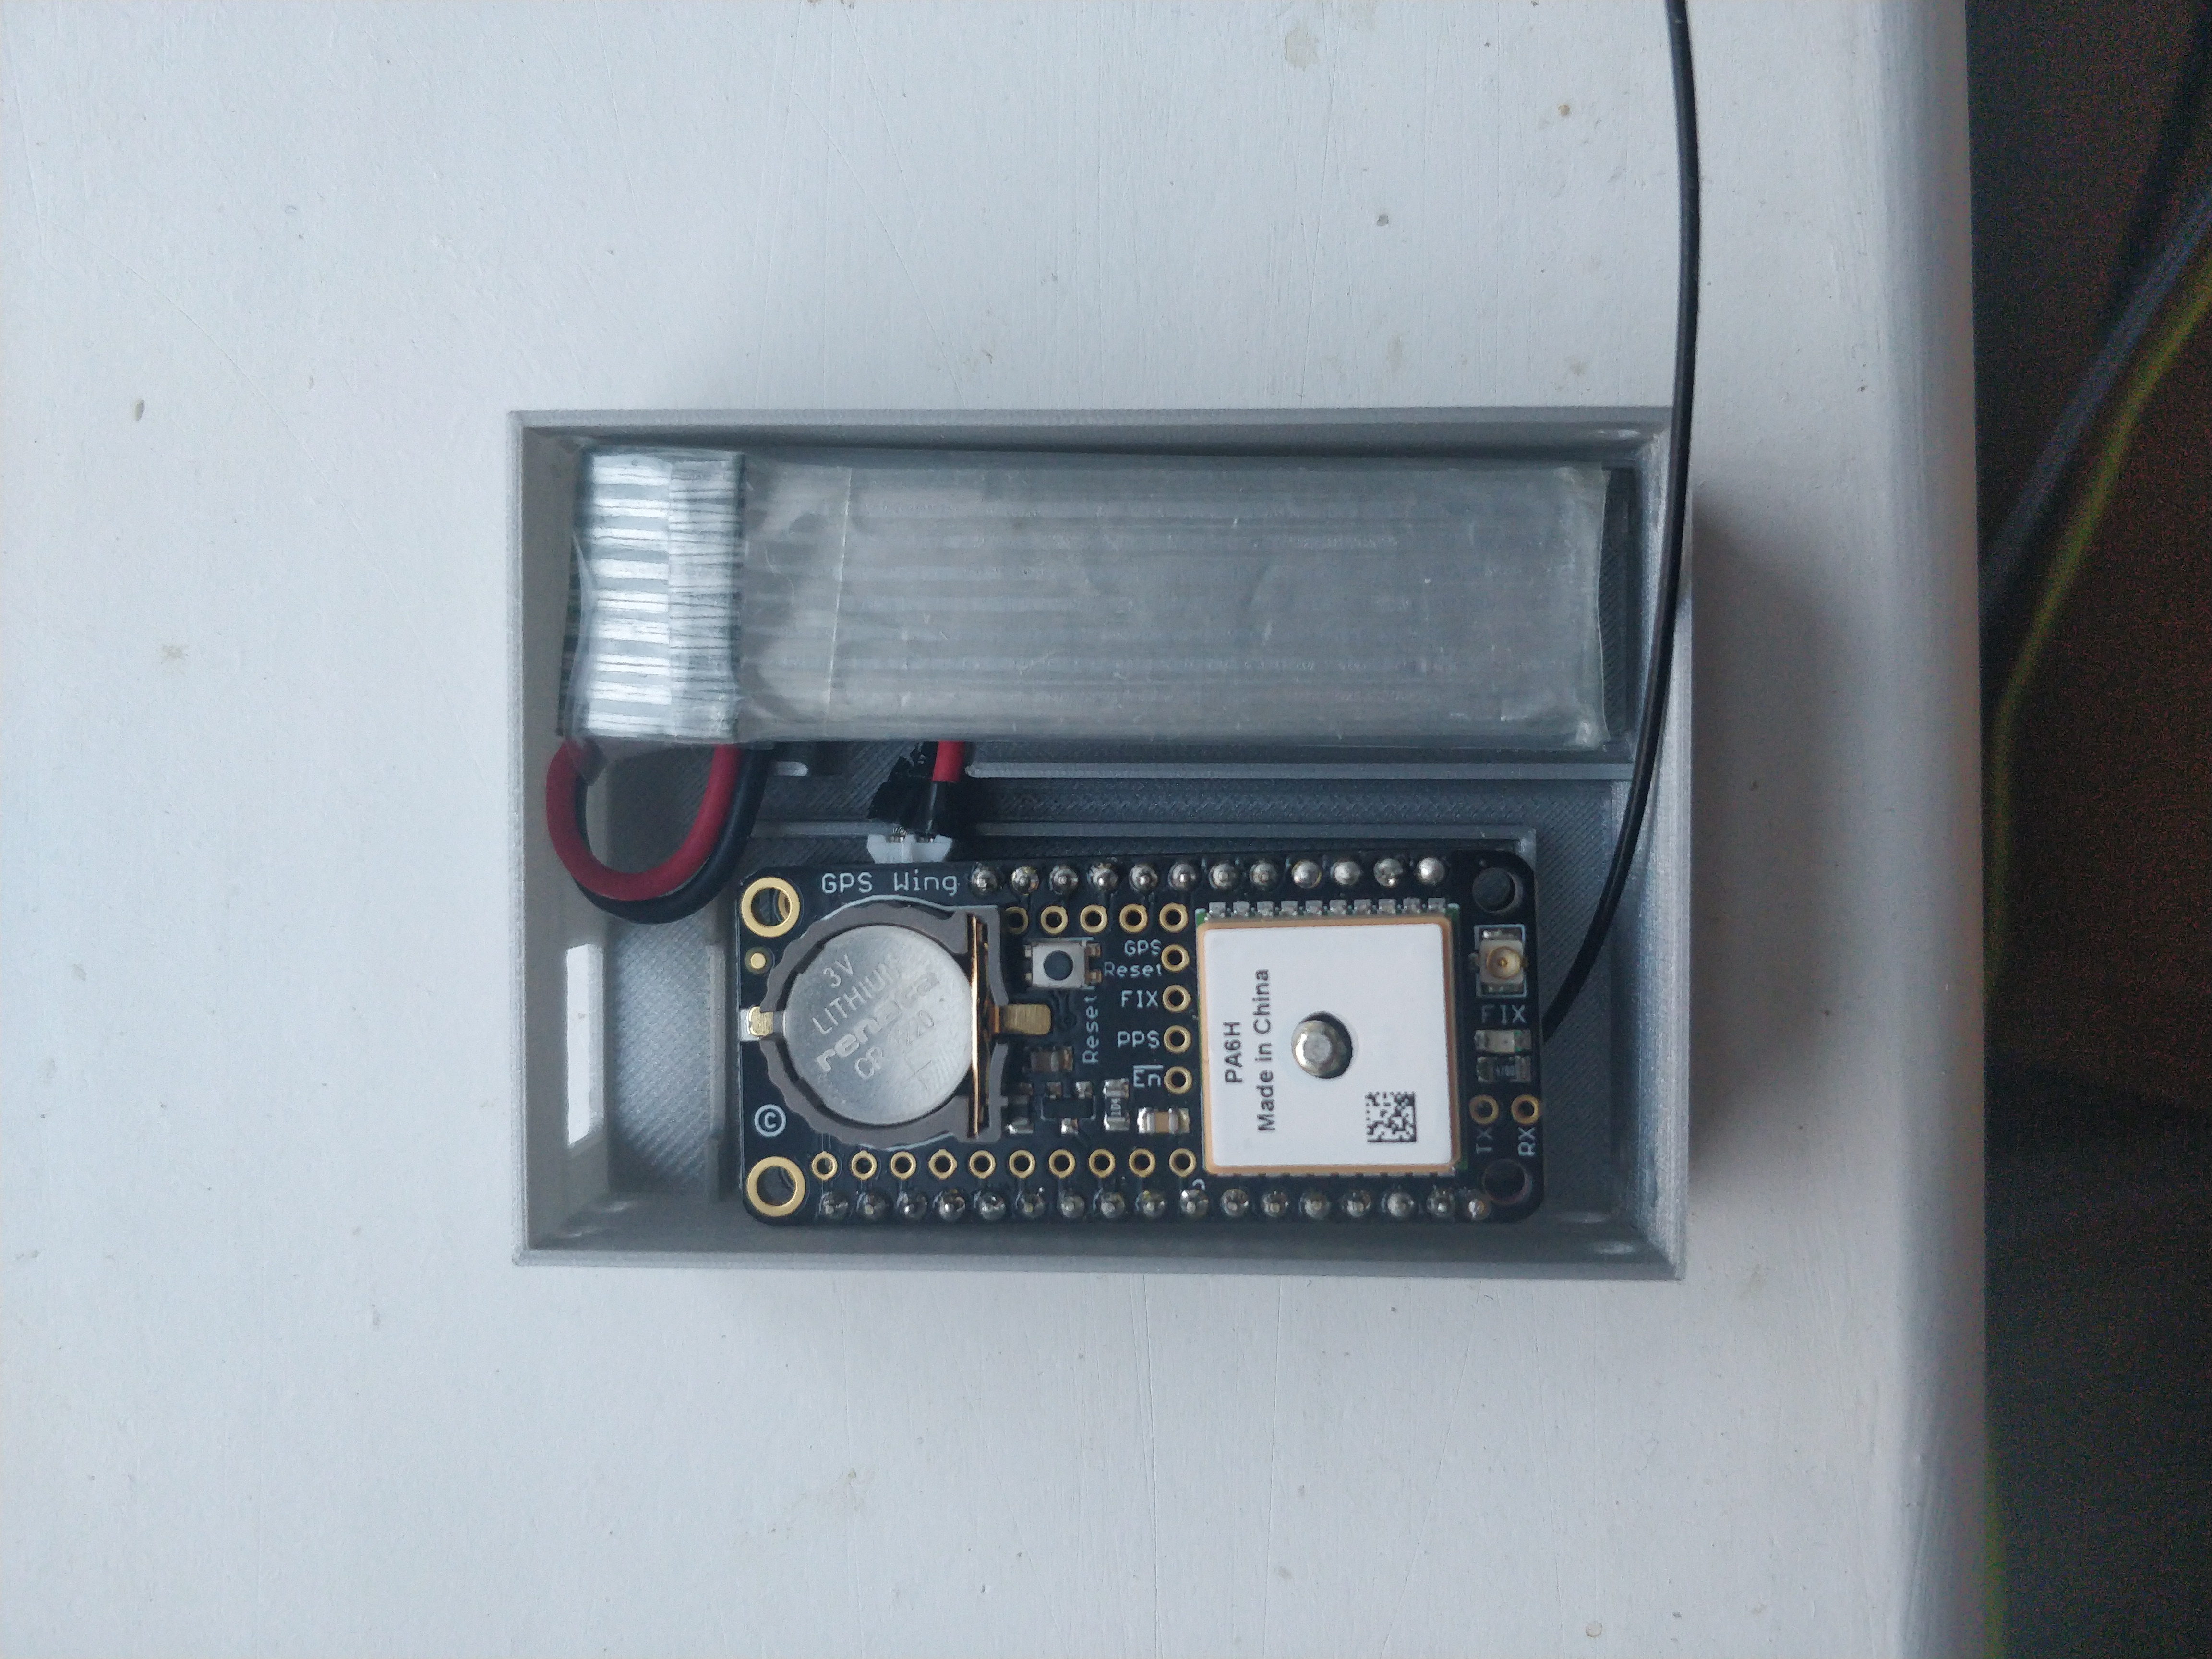
\includegraphics[width=\textwidth]{../figures/Pics/secondcase0.jpg}
            \caption{Case overview}
        \end{subfigure}
        \vskip\baselineskip
        \hspace*{\fill}
        \begin{subfigure}[b]{0.3\textwidth}
            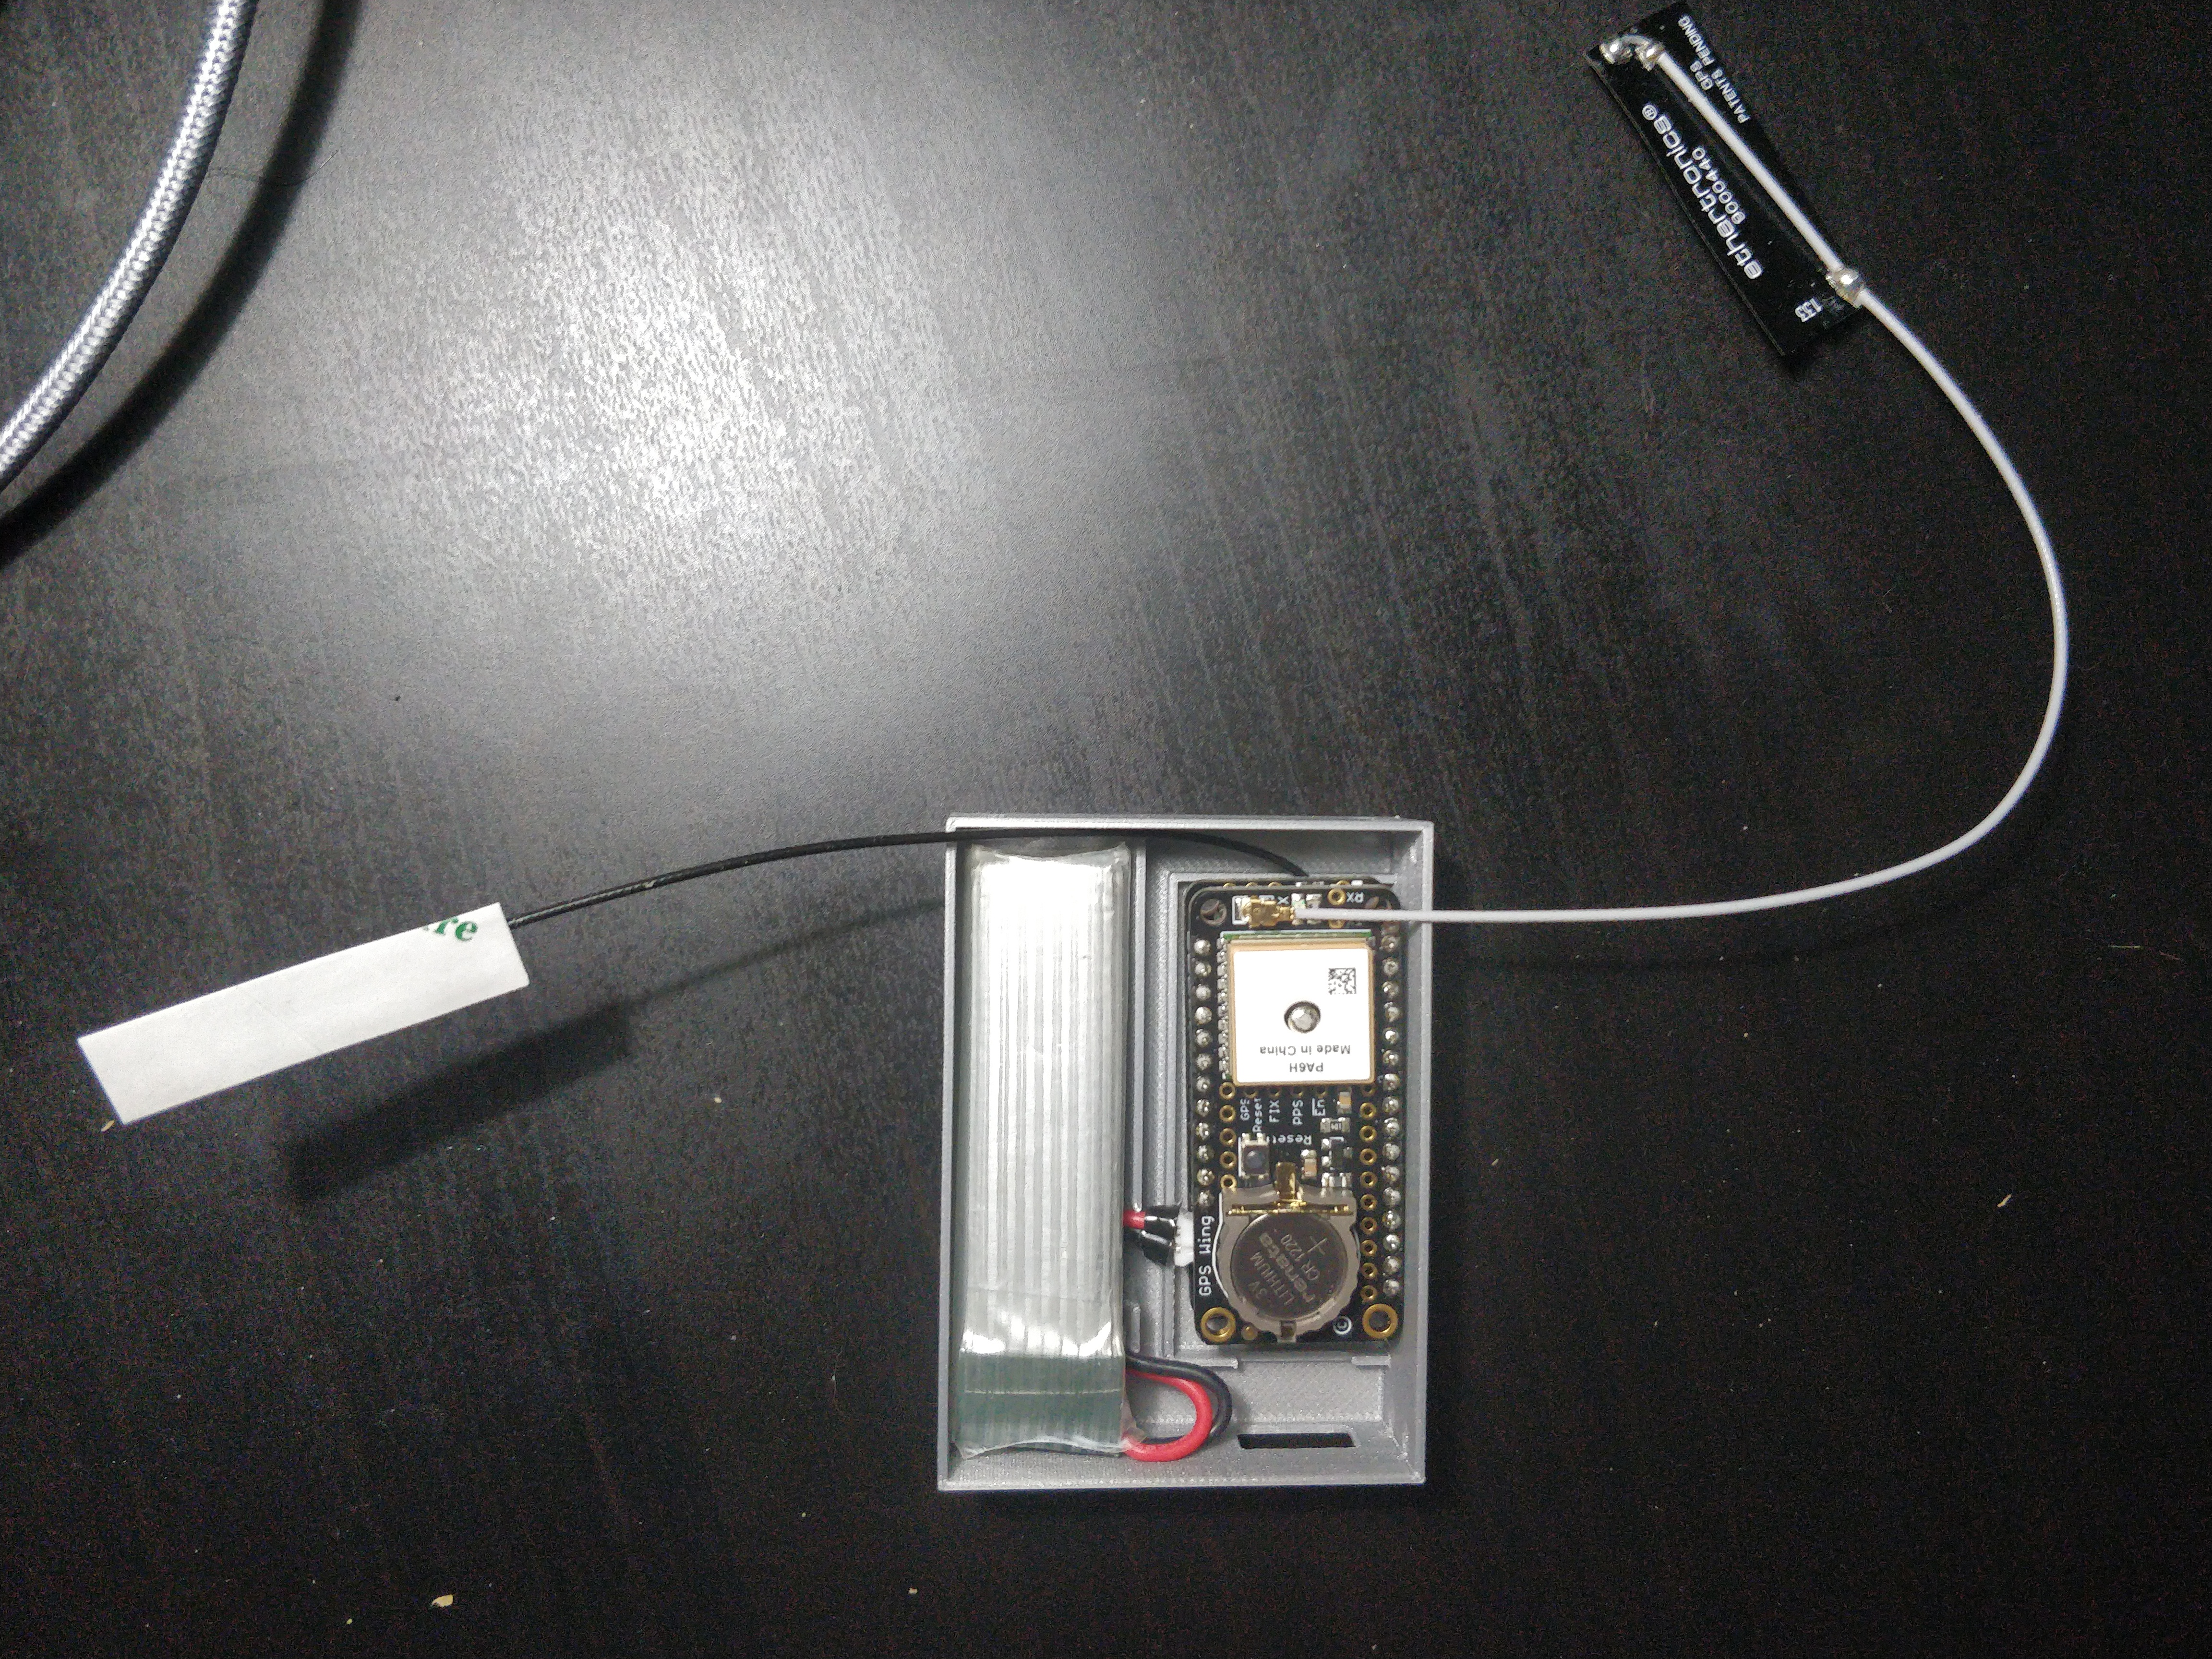
\includegraphics[angle=90,width=\textwidth]{../figures/Pics/secondcase1.jpg}
            \vspace{5pt}
            \caption{Case with antennae}            
            \label{fig:case2antennasplay}
        \end{subfigure}
        \hfill
        \begin{subfigure}[b]{0.3\textwidth}  
            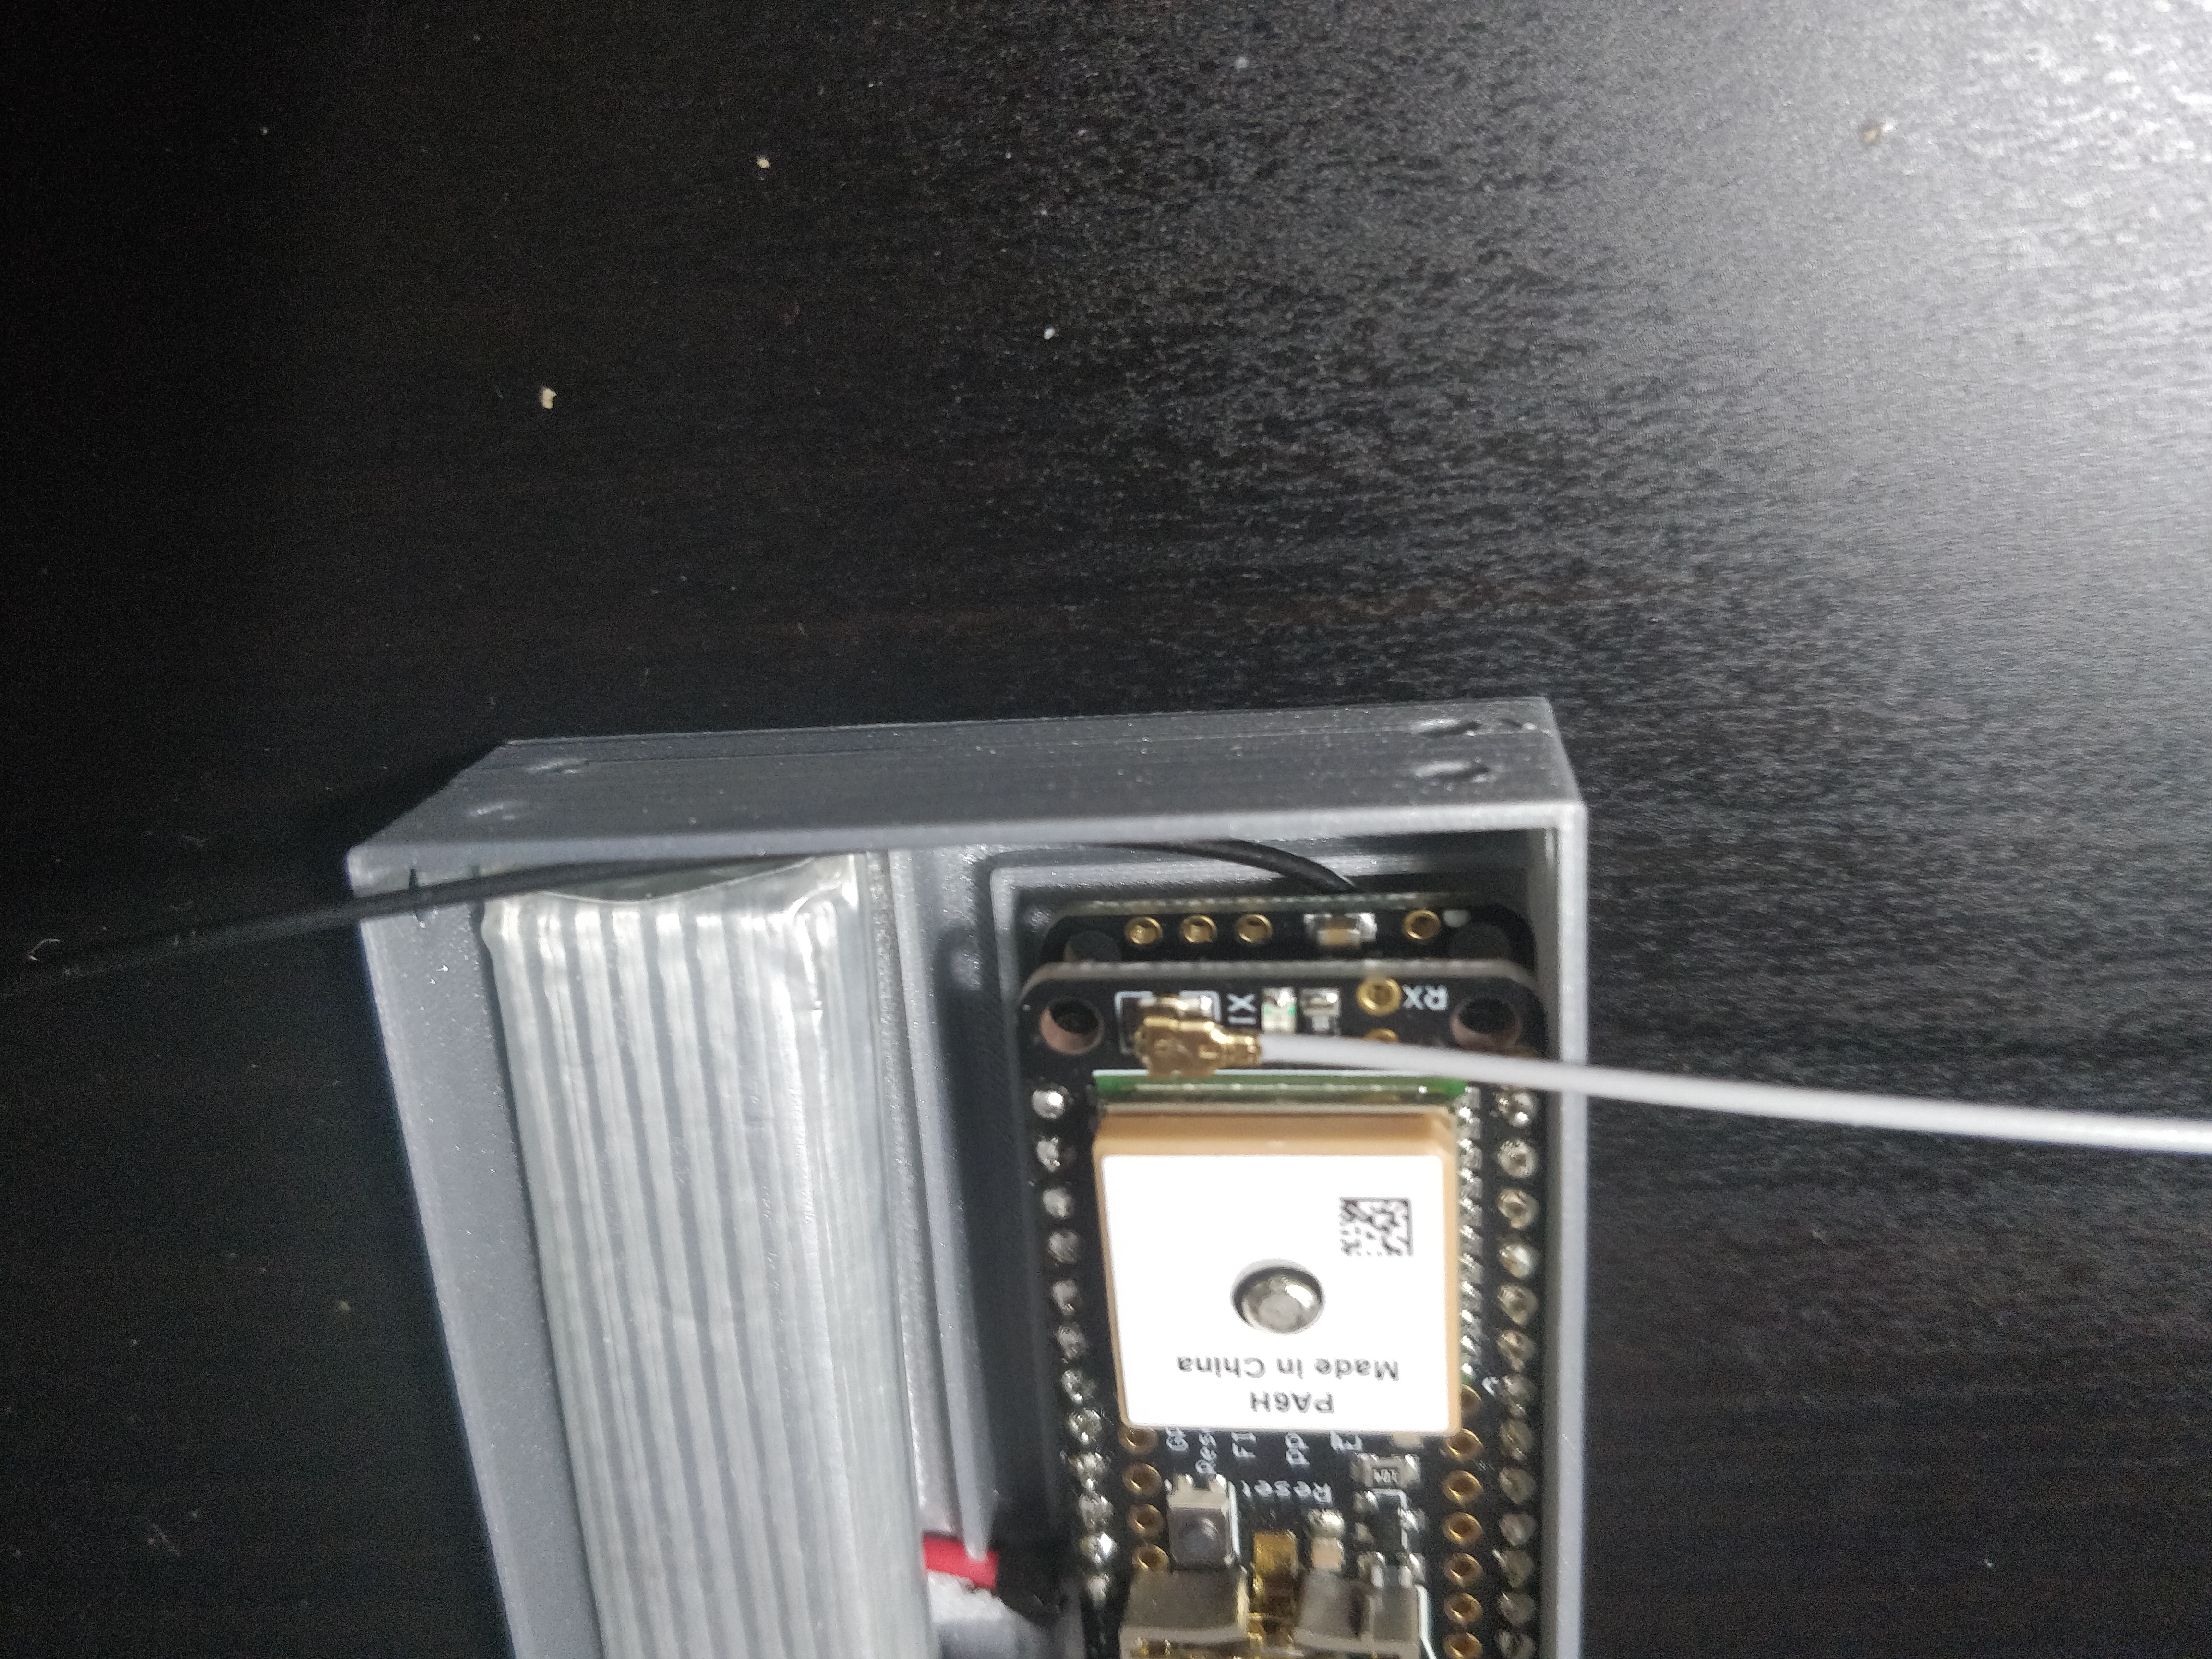
\includegraphics[angle=90,width=\textwidth]{../figures/Pics/secondcase2.jpg}
            \vspace{5pt}
            \caption{Antenna raising issue}                    
            \label{fig:case2antennaissue}
        \end{subfigure}
        \hspace*{\fill}
        \vskip\baselineskip
        \hspace*{\fill}
        \begin{subfigure}[b]{0.3\textwidth}   
            \captionsetup{justification=centering}
            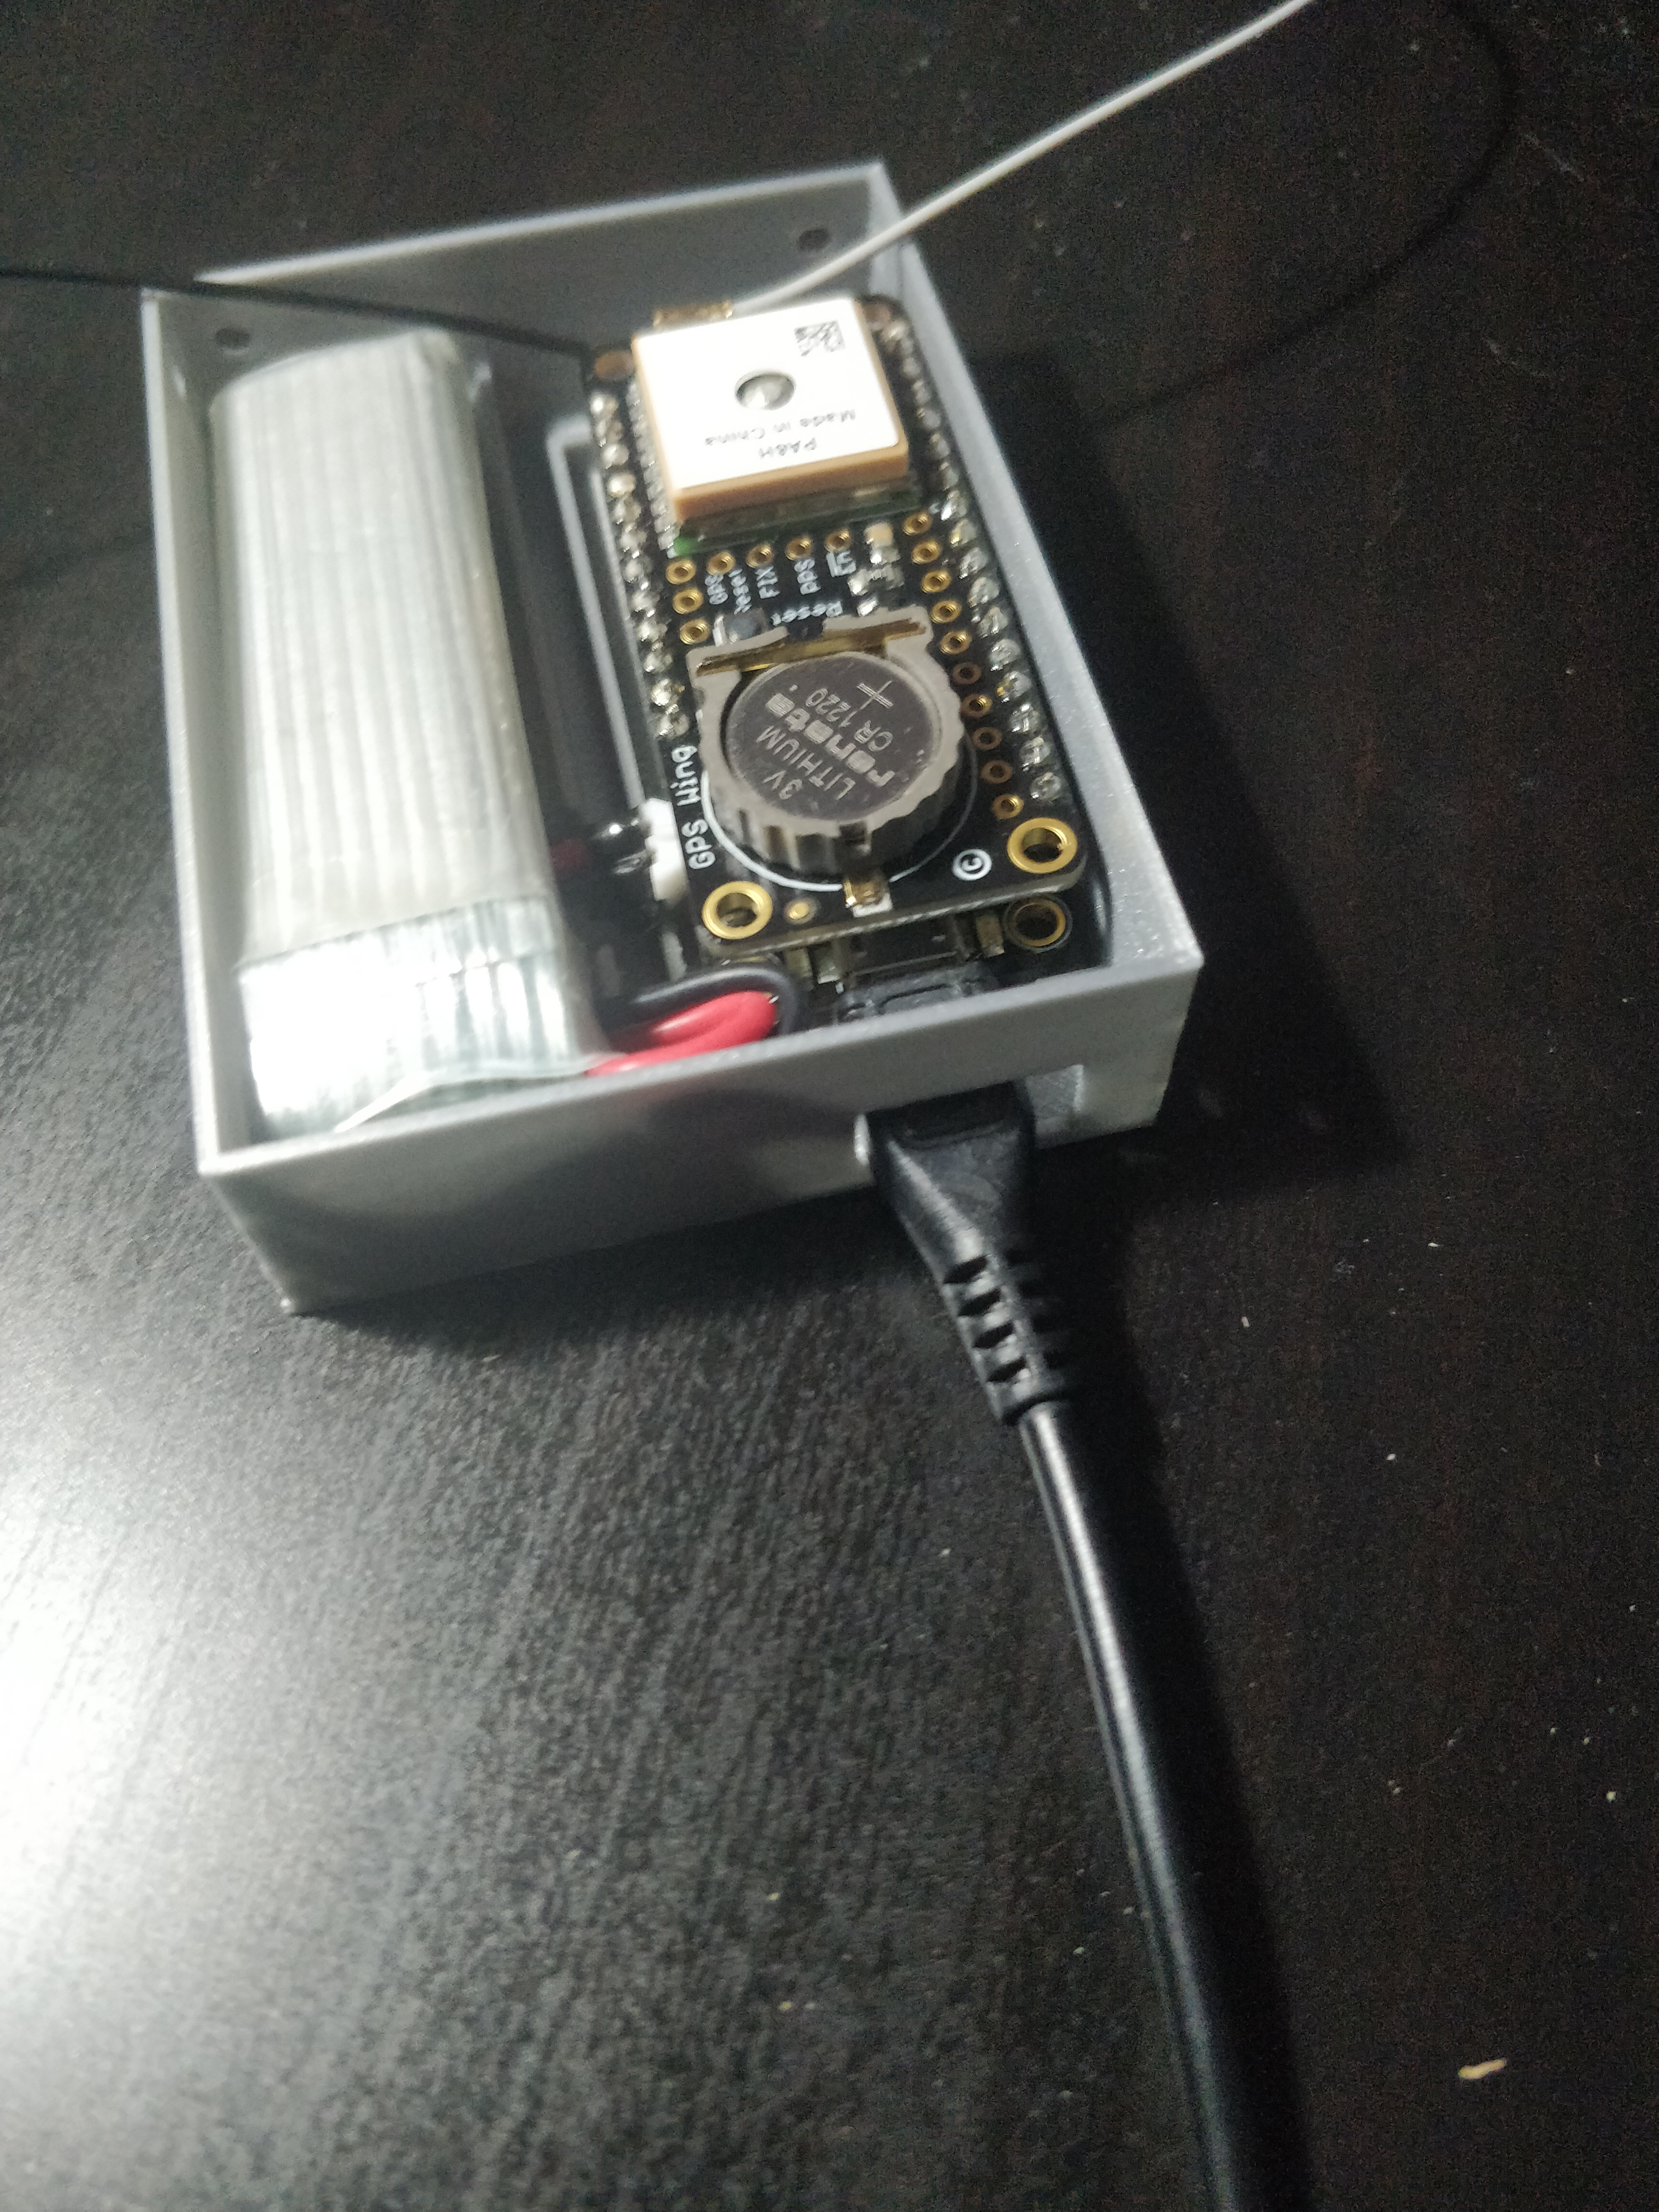
\includegraphics[width=\textwidth]{../figures/Pics/secondcase3.jpg}
            \vspace{1pt}
            \caption{Angled front view with \acrshort{usb} connection}
        \end{subfigure}
        \hfill
        \begin{subfigure}[b]{0.3\textwidth}           
            \captionsetup{justification=centering}
            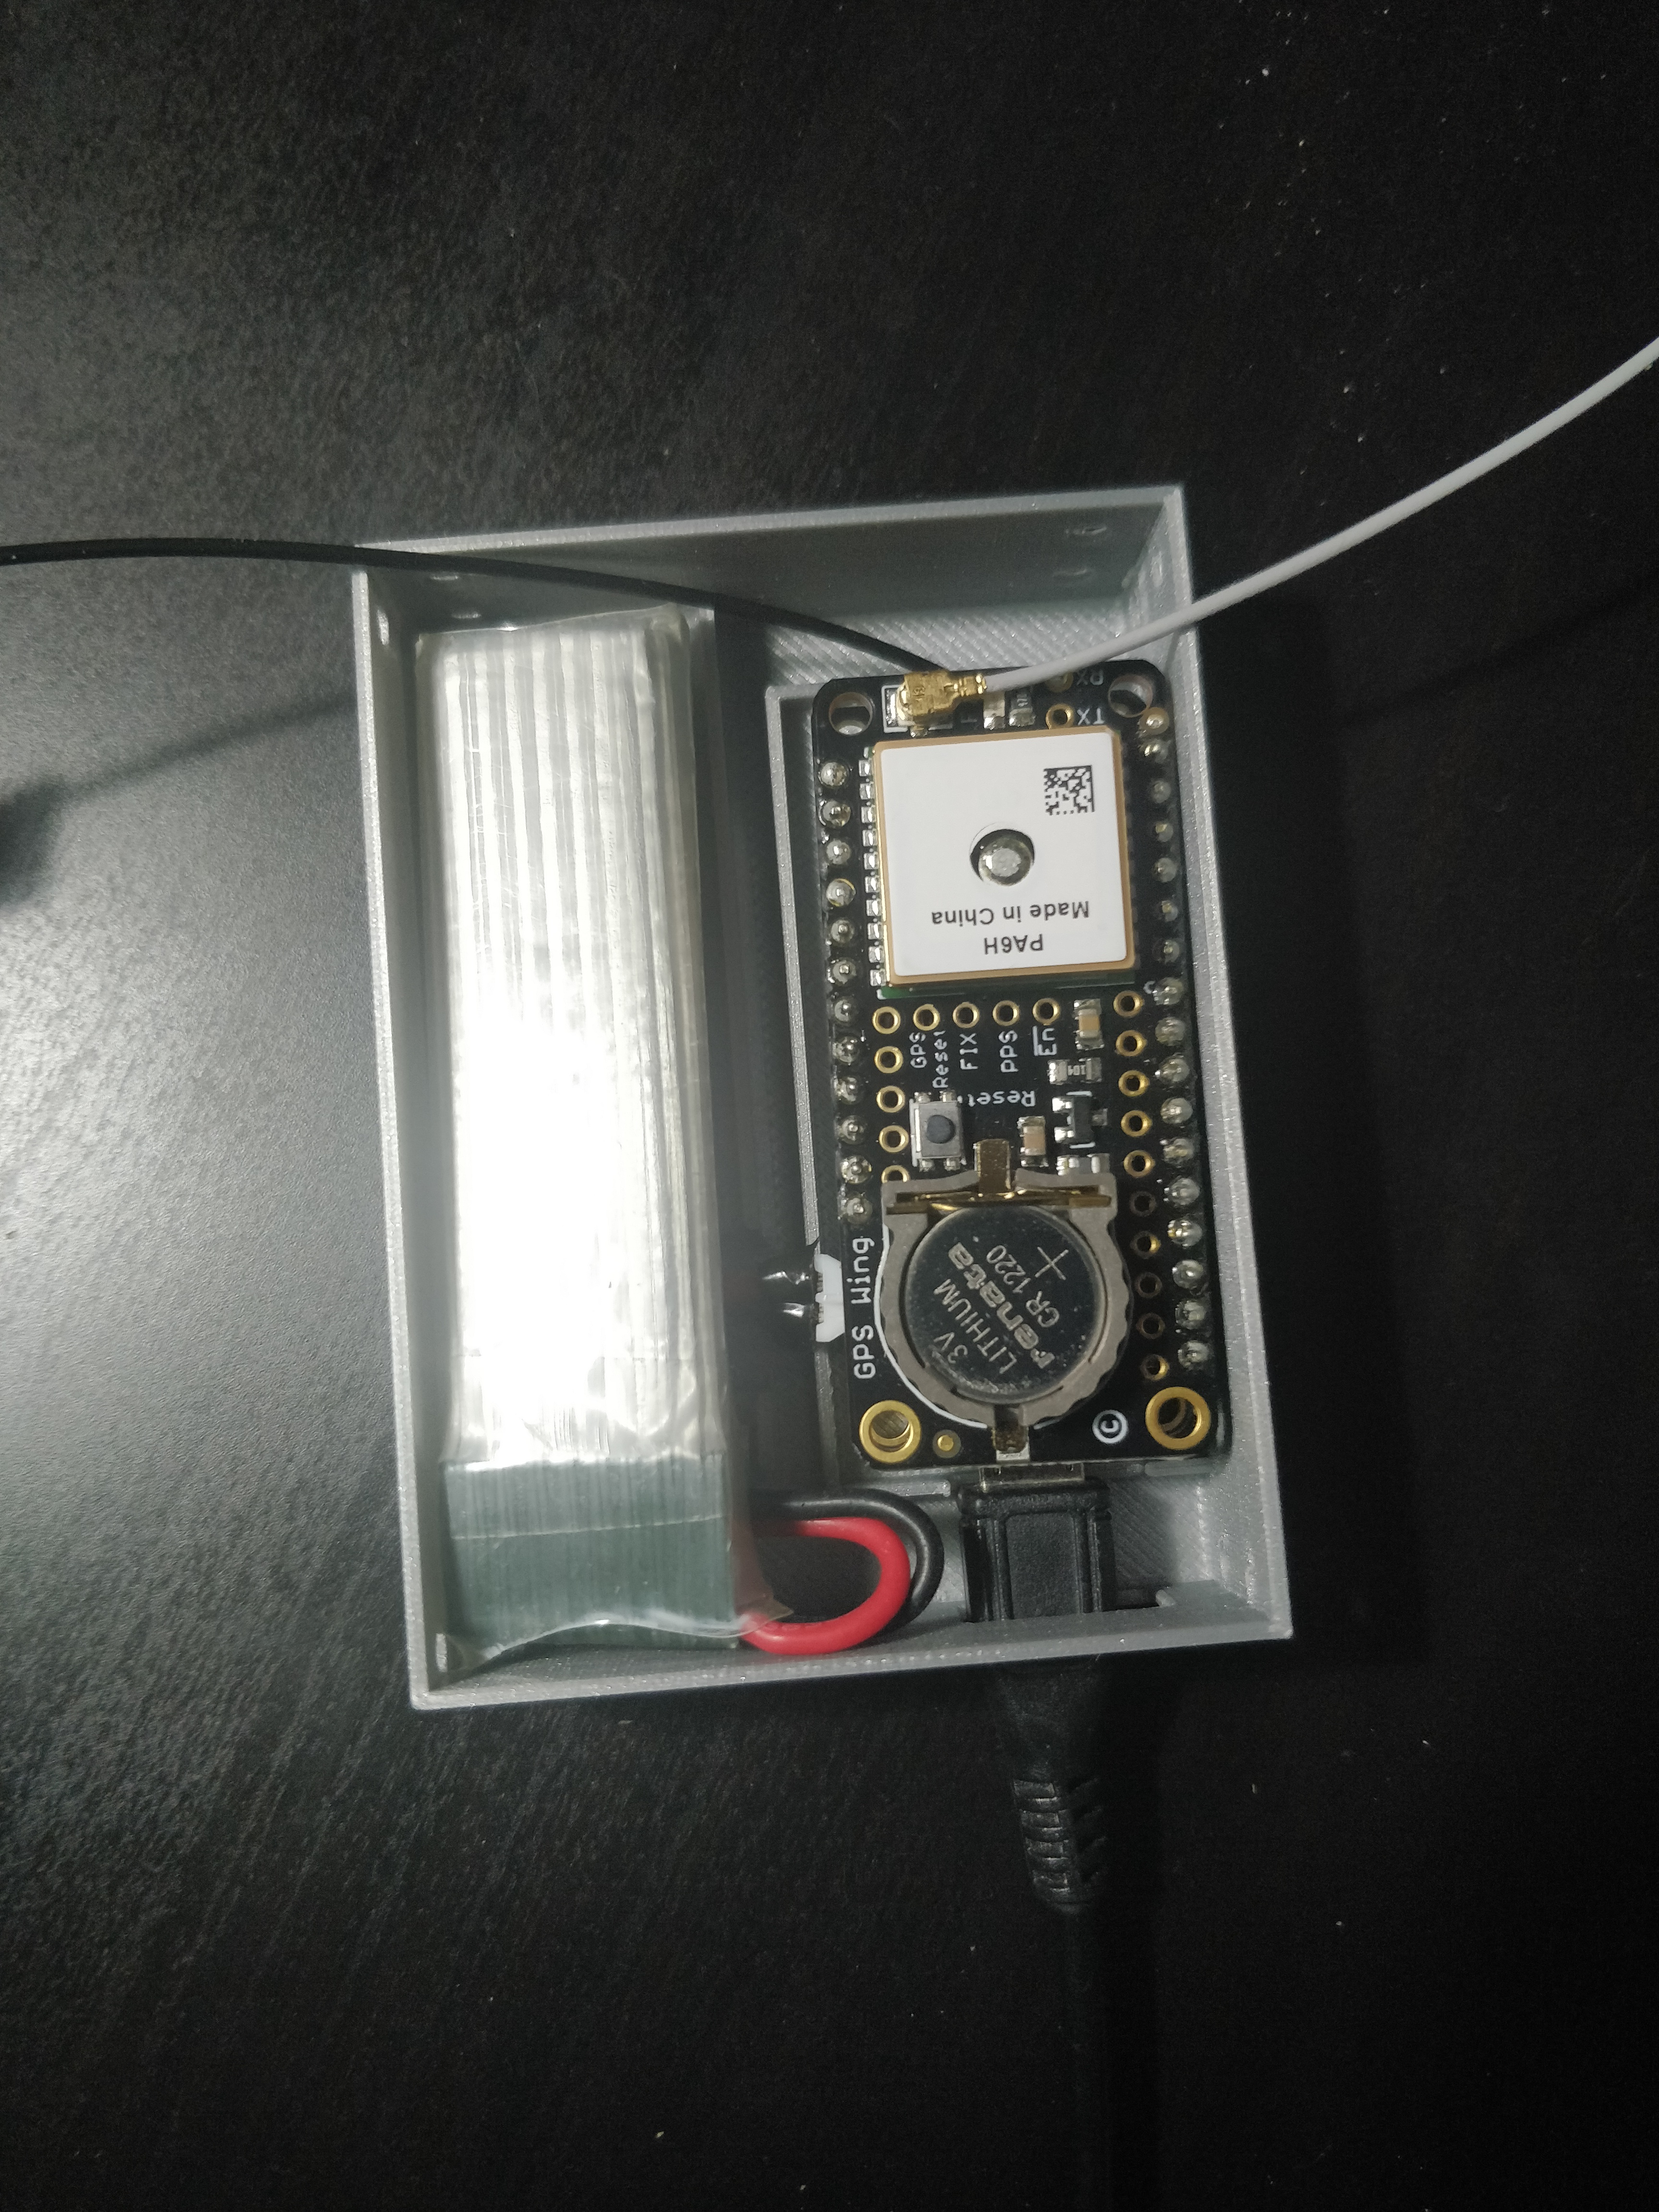
\includegraphics[width=\textwidth]{../figures/Pics/secondcase4.jpg}
            \vspace{5pt}
            \caption{Top view with \acrshort{usb} connection}
        \end{subfigure}
        \hspace*{\fill}
    \end{figure}
    \vfill
    \clearpage

    % \begin{figure}[H]        
    %     \label{case2dwg}
    %     \caption{Case 2 dimensional drawing}
    %     \includegraphics[angle=-90,width=\textwidth]{../../Design/case2.pdf}
    % \end{figure}   

    % \begin{figure}[H]        
        % \includepdf[pagecommand={},angle=-90,scale=0.9,pagecommand=\section{Case 2 dimensional drawing \label{fig:case2dwg}}]{../../Design/case2.pdf}
        % \label{fig:case2dwg}
    % \end{figure}
    % \clearpage

    \begin{figure}[H]      
        \caption{Case 2 dimensional drawings}
        \includepdf[pagecommand={},angle=-90,scale=0.9]{../../Design/case2.pdf}  
        \label{fig:case2dwg}
    \end{figure}
   


\begin{landscape}

\chapter{Purchasing lists}

    \begin{xltabular}{\linewidth}{|cYccccc|}
        \caption{Preliminary hardware list} \label{table:prelimhardwarelist} \\
        \hline

        \rowcolor{tableh2}
        Part & Description & Quantity  & Price per unit & Supplier & SKU & Web link \\
        \endfirsthead

        \caption{Preliminary hardware list (cont.)}\\
        \hline
        \rowcolor{tableh2}
        Part & Description & Quantity  & Price per unit & Supplier & SKU & Web link \\
        \endhead
        \endfoot

        \hline
        \rowcolor{tableh1}
        \multicolumn{7}{|c|}{Common requirement} \\
        \hline
        SX1262 LoRa HAT & LoRa radio for the Raspberry Pi & 1   & 28.10 & PiHut & WAV-16806 & \href{https://thepihut.com/products/sx1262-lora-hat-for-raspberry-pi-868mhz-for-europe-asia-africa}{Link \faExternalLink} \\
        \hline
        500mAh LiPo battery	& &	1 &	6.00	& PiHut &	105189 &	\href{https://thepihut.com/products/500mah-3-7v-lipo-battery}{Link \faExternalLink} \\
        \hline
        \rowcolor{tableh1}
        \multicolumn{7}{|c|}{Transmitter Set 1} \\
        \hline
        Challenger RP2040 &	microcontroller with lora radio	& 1 &	21.5	& PiHut	& 104944	& \href{https://thepihut.com/products/challenger-rp2040-lora-868mhz}{Link \faExternalLink} \\
        \hline
        GPS Featherwing &	gps module (uart)	& 1 &	24.6 &	PiHut &	ADA3133 &	\href{https://thepihut.com/products/adafruit-ultimate-gps-featherwing}{Link \faExternalLink} \\
        \hline
        \rowcolor{tableh1}
        \multicolumn{7}{|c|}{Transmitter Set 2 - I\textsuperscript{2}C alternative} \\
        \hline
        Feather RP2040 &	microcontroller	& 1	& 11.4	& PiHut &	ADA4884	& \href{https://thepihut.com/products/adafruit-feather-rp2040}{Link \faExternalLink} \\
        \hline
        LoRa Featherwing &	lora radio (i2c) &	1	& 19.5 &	PiHut &	ADA3231 &	\href{https://thepihut.com/products/adafruit-lora-radio-featherwing-rfm95w-900-mhz}{Link \faExternalLink} \\
        \hline
        GPS breakout &	gps module (i2c) &	1 &	29.7 &	PiHut &	PIM525 &	\href{https://thepihut.com/products/pa1010d-gps-breakout}{Link \faExternalLink} \\
        \hline
        uFL connector &	to get an antenna onto the lora board &	5	& 0.8 &	PiHut	& ADA1661 &	\href{https://thepihut.com/products/ufl-smt-antenna-connector}{Link \faExternalLink} \\
        \hline
        \rowcolor{tableh1}
        \multicolumn{7}{|c|}{Antenna Options} \\
        \hline
        W3013 & 	ceramic  & 	2 & 	1.48 & 	Mouser & 	673-W3013	 & \href{https://www.mouser.co.uk/ProductDetail/Pulse-Electronics/W3013?qs=sk8jCzc\%252BkzSRDEaf6KYAUA\%3D\%3D}{Link \faExternalLink} \\
        \hline
        PIOV008NRAA-100	 & strip with ufl &  	1 & 	1.87 & 	Mouser & 	523-PIOV008NRAA-100	 & \href{https://www.mouser.co.uk/ProductDetail/Amphenol-MCP/PIOV008NRAA-100?qs=GedFDFLaBXFCaCiGvxFhnA\%3D\%3D}{Link \faExternalLink} \\
        \hline
        318020612 & 	Outdoor antenna - N male	 & 1	 & 30.8 & 	Mouser & 	713-318020612 & 	\href{https://www.mouser.co.uk/ProductDetail/Seeed-Studio/318020612?qs=TuK3vfAjtkUc5jgrDpnp\%252Bw\%3D\%3D}{Link \faExternalLink} \\
        \hline
        &   amazon option with included cable and adapter	 & 1	 & 30.99 & 	Amazon	 & &	\href{https://amzn.eu/d/daYwpxw}{Link \faExternalLink} \\
        \hline
        CAB.951	 & N female - SMA male, 1m	 & 1	 & 17.13 & 	Mouser & 	960-CAB.951	 & \href{https://www.mouser.co.uk/ProductDetail/Taoglas/CAB.951?qs=RuW\%2Fu\%252BNMQmvLr59ScsVBcw\%3D\%3D}{Link \faExternalLink} \\
        \hline
        &  much cheaper amazon option & 	1 & 	11.98	 & Amazon	 & &	\href{https://amzn.eu/d/d8hsE0k}{Link \faExternalLink} \\
        \hline
        Pigtail Antenna	 & only if none of the other options work & 	2	 & 4.9 & 	PiHut & 	105078	 & \href{https://thepihut.com/products/lora-antenna-with-pigtail-868mhz-black}{Link \faExternalLink} \\
        \hline
        Raspberry Pi & 	it's okay I actually own a Pi3 & 	1	 & 219.99	 & Amazon	& & 	\href{https://amzn.eu/d/7W5NpuZ}{Link \faExternalLink} \\
        \hline
    \end{xltabular}

    \begin{xltabular}{\linewidth}{|cYccccc|}
        \caption{Updated hardware list} \label{table:updatedhardwarelist}\\
        \hline
        \rowcolor{tableh2}
        Part & Description & Quantity  & Price per unit & Supplier & SKU & Web link \\
        \endfirsthead

        \caption{Updated hardware list (cont.)}\\
        \hline
        \rowcolor{tableh2}
        Part & Description & Quantity  & Price per unit & Supplier & SKU & Web link \\
        \endhead
        \endfoot

        \hline
        \rowcolor{tableh1}
        \multicolumn{7}{|c|}{Transmitter} \\
        \hline
        3178	 & Feather M0 LoRa & 1 & 	30.76 & 	 Mouser & 	485-3178 & 	\href{https://www.mouser.co.uk/ProductDetail/Adafruit/3178?qs=TlVEbN\%2FgKDkhUZkXCJivzw\%3D\%3D}{Link \faExternalLink} \\
        \hline
        3133	 & GPS Featherwing	 & 1	 & 21.96	  & 	Mouser & 	485-3133 & 	\href{https://www.mouser.co.uk/ProductDetail/Adafruit/3133?qs=TlVEbN\%2FgKDmpiId5nasRCA\%3D\%3D}{Link \faExternalLink} \\
        \hline
        & Pimoroni equivalent & 	1	 & 24.6		 & Pimoroni & 	ADA3133 & 	\href{https://shop.pimoroni.com/products/adafruit-ultimate-gps-featherwing?variant=21438274887}{Link \faExternalLink} \\
        \hline

        \rowcolor{tableh1}
        \multicolumn{7}{|c|}{Receiver} \\
        \hline
        3231	 & LoRa Featherwing & 	1	 & 18.68	 & 	Digikey	 & 1528-1741-ND	 & \href{https://www.digikey.co.uk/en/products/detail/adafruit-industries-llc/3231/6193593}{Link \faExternalLink} \\
        \hline
        & Equivalent	 & 1	 & 19.5	 & 	Pimoroni	 & ADA3231 & 	\href{https://shop.pimoroni.com/products/adafruit-lora-radio-featherwing-rfm95w-900-mhz-radiofruit?variant=2089110306826}{Link \faExternalLink} \\
        \hline
        & Bonnet OLED alternative	 & 1	 & 31.8		 & Pimoroni & 	ADA4074	 & \href{https://shop.pimoroni.com/products/adafruit-lora-radio-bonnet-with-oled-rfm95w-915mhz-radiofruit?variant=27912635220051}{Link \faExternalLink} \\
        \hline
        & + headers & 	1 & 	2.1	 & 	Pimoroni	 & COM0003 & 	\href{https://shop.pimoroni.com/products/booster-header?variant=47414520906}{Link \faExternalLink} \\
        \hline

        \rowcolor{tableh1}
        \multicolumn{7}{|c|}{Accessories} \\
        \hline
        2258	 & Pi Case & 	1 & 	7	 & 	Mouser	 & 485-2258	 & \href{https://www.mouser.co.uk/ProductDetail/Adafruit/2258?qs=GURawfaeGuAHsbLMi7envw\%3D\%3D}{Link \faExternalLink} \\
        \hline
        &  Equivalent	 & 1	 & 7.8	 & 	Pimoroni	 & ADA2258	 & \href{https://shop.pimoroni.com/products/adafruit-raspberry-pi-b-case-smoke-base-w-clear-top?variant=1005886429}{Link \faExternalLink} \\
        \hline
        4410	 & lipo (jst) charger	 & 1 & 	5.24	 & Mouser	 & 485-4410 & 	\href{https://www.mouser.co.uk/ProductDetail/Adafruit/4410?qs=wnTfsH77Xs5n1kx9qVo63A\%3D\%3D}{Link \faExternalLink} \\
        \hline
        2830 & 	stacking headers 1st level & 	1 & 		1.1	 & Mouser	 & 485-2830 & 	\href{https://www.mouser.co.uk/ProductDetail/Adafruit/2830?qs=xE9dPqTLfL4XzxEZXTz\%252BEA\%3D\%3D}{Link \faExternalLink} \\
        \hline
        & Equivalent	 & 1	 & 1.1	 & 	Pimoroni	 & ADA2830	 & \href{https://shop.pimoroni.com/products/feather-stacking-headers-12-pin-and-16-pin-female-headers?variant=13709873863}{Link \faExternalLink} \\
        \hline
        2886	 & stacking headers base	 & 1	 & 0.836	 & 	Mouser & 	485-2886 & 	\href{https://www.mouser.co.uk/ProductDetail/Adafruit/2886?qs=xE9dPqTLfL61eEvyw283TQ\%3D\%3D}{Link \faExternalLink} \\
        \hline
        &   Equivalent	 & 1	 & 1.2	 & 	Pimoroni & 	ADA2886	 & \href{https://shop.pimoroni.com/products/feather-header-kit-12-pin-and-16-pin-female-header-set?variant=13710014791}{Link \faExternalLink} \\
        \hline

        \rowcolor{tableh1}
        \multicolumn{7}{|c|}{Battery} \\
        \hline
        4714 & 	JST PH Female jumper	 & 1 & 	0.836 & 		Mouser & 	485-4714 & 	\href{https://www.mouser.co.uk/ProductDetail/Adafruit/4714?qs=hd1VzrDQEGi2qAbAJE0pRQ\%3D\%3D}{Link \faExternalLink} \\
        \hline
        RS PRO battery	 & LiPo 1.8Ah	 & 1	 & 10.86	 & RS & 	144-9405 & 	\href{https://uk.rs-online.com/web/p/speciality-size-rechargeable-batteries/1449405}{Link \faExternalLink} \\
        \hline
        Alternative  & 1.2mAh, doesn't require jumper or housing 	 & 1	 & 9.9	 & 	Pimoroni & 	BAT00044	 & \href{https://shop.pimoroni.com/products/lipo-battery-pack?variant=20429082183}{Link \faExternalLink} \\
        \hline
        PHR-2	 & JST PH Female connector housing	 & 1	 & 0.66	 & RS	 & 820-1466 & 	\href{https://uk.rs-online.com/web/p/wire-housings-plugs/8201466}{Link \faExternalLink} \\
        \hline

        \rowcolor{tableh1}
        \multicolumn{7}{|c|}{Antenna} \\
        \hline
        ANT-868-CPA	 & ceramic 	 & 1	 & 2.97	  & Mouser	 & 712-ANT-868-CPA & 	\href{https://www.mouser.co.uk/ProductDetail/Linx-Technologies/ANT-868-CPA?qs=wnTfsH77Xs69O4Svqy49rA\%3D\%3D}{Link \faExternalLink} \\
        \hline
        PIOV008NRAA-100	 & strip with ufl  & 	1	 & 1.87	 & Mouser	 & 523-PIOV008NRAA-100 & 	\href{https://www.mouser.co.uk/ProductDetail/Amphenol-MCP/PIOV008NRAA-100?qs=GedFDFLaBXFCaCiGvxFhnA\%3D\%3D}{Link \faExternalLink} \\
        \hline
        318020612 & 	Outdoor antenna - N male	 & 1	 & 30.8 & 	Mouser	 & 713-318020612	 & \href{https://www.mouser.co.uk/ProductDetail/Seeed-Studio/318020612?qs=TuK3vfAjtkUc5jgrDpnp\%252Bw\%3D\%3D}{Link \faExternalLink} \\
        \hline
        CAB.951	 & N female - SMA male, 1m	 & 1	 & 17.13 & 	Mouser	 & 960-CAB.951	 & \href{https://www.mouser.co.uk/ProductDetail/Taoglas/CAB.951?qs=RuW\%2Fu\%252BNMQmvLr59ScsVBcw\%3D\%3D}{Link \faExternalLink} \\
        \hline
        CONUFL001-SMD-T	 & uFL connector	 & 5	 & 0.625	 & 	Mouser	 & 712-CONUFL001-SMD-T & 	\href{https://www.mouser.co.uk/ProductDetail/Linx-Technologies/CONUFL001-SMD-T?qs=EU6FO9ffTwfRdkBeQTdJWQ\%3D\%3D}{Link \faExternalLink} \\
        \hline
        CASMA-UFL-1	 & uFL to SMA F	 & 2	 & 8.71	 & Mouser	 & 125-CASMA-UFL-1	 & \href{https://www.mouser.co.uk/ProductDetail/MultiTech/CASMA-UFL-1?qs=7MVldsJ5UawLWQzcvLUp6A\%3D\%3D}{Link \faExternalLink} \\
        \hline
        & Equivalent	 & 2	 & 3.9	 & 	Pimoroni	 & ADA851	 & \href{https://shop.pimoroni.com/products/adafruit-sma-to-ufl-u-fl-ipx-ipex-rf-adapter-cable?variant=433911117}{Link \faExternalLink} \\
        \hline

        \rowcolor{tableh1}
        \multicolumn{7}{|c|}{Additional Antennae} \\
        \hline
        W3214	 & ceramic  & 	1 & 	2.08	 & 	Mouser	 & 673-W3214 & 	\href{https://www.mouser.co.uk/ProductDetail/Pulse-Electronics/W3214?qs=l7cgNqFNU1gaMT1NL8sSIA\%3D\%3D}{Link \faExternalLink} \\
        \hline
        M620720 & 	ceramic  & 	1	 & 1.73	 & 	Mouser & 	581-M620720 & 	\href{https://www.mouser.co.uk/ProductDetail/Ethertronics-KYOCERA-AVX/M620720?qs=MLItCLRbWsxW2ijaVr6ojw\%3D\%3D}{Link \faExternalLink} \\
        \hline
        W3013	 & ceramic 	 & 1	 & 1.48	 & 	Mouser	 & 673-W3013 & 	\href{https://www.mouser.co.uk/ProductDetail/Pulse-Electronics/W3013?qs=sk8jCzc\%252BkzSRDEaf6KYAUA\%3D\%3D}{Link \faExternalLink} \\
        \hline

    \end{xltabular}

    \begin{xltabular}{\linewidth}{|Ycccccc|}
        \caption{Antennae list} \label{table:antennaelist} \\
        \hline

        \rowcolor{tableh2}
        Description & Part & Name  & Price & Supplier & SKU & Web link \\
        \endfirsthead

        \caption{Preliminary hardware list (cont.)}\\
        \hline
        \rowcolor{tableh2}
        Part & Description & Quantity  & Price per unit & Supplier & SKU & Web link \\
        \endhead
        \endfoot

        \hline
        Original antenna: & 	318020612 & 	Outdoor antenna - N male & 	30.8 & 	Mouser	 & 713-318020612 & 	\href{https://www.mouser.co.uk/ProductDetail/Seeed-Studio/318020612?qs=TuK3vfAjtkUc5jgrDpnp\%252Bw\%3D\%3D}{Link \faExternalLink} \\
        \hline
        Suggested replacement:	 & 318020690	 & 5.8dBi antenna & 	41.24 & 	Farnell	 & 4060414 & 	\href{https://uk.farnell.com/seeed-studio/318020690/antenna-fiberglass-863-to-870mhz/dp/4060414}{Link \faExternalLink} \\
        \hline
        Cheaper alternative:	 & 318020708	 & 3dBi antenna	 & 24.72	 & Farnell	 & 4060419 & 	\href{https://uk.farnell.com/seeed-studio/318020708/antenna-fiberglass-860-to-930mhz/dp/4060419}{Link \faExternalLink} \\
        \hline
        Lora antenna	 & 211140-0100	 & 0.3dBi at 868, 38mm	 & 1.7	 & Farnell	 & 3498957 & 	\href{https://uk.farnell.com/molex/211140-0100/ism-antenna-902-928mhz-1dbi/dp/3498957?st=ism\%20antenna}{Link \faExternalLink} \\
        \hline
        Additional lora antenna	 & 1002289F0-AA10L0200 & 	1.8 dBi & 	3.95 & 	Farnell	 & 3407000 & 	\href{https://uk.farnell.com/avx/1002289f0-aa10l0200/fpc-embedded-antenna-2-69ghz-4/dp/3407000}{Link \faExternalLink} \\
        \hline
        gps antenna	 & 9000440	 &  & 	1.79	 & Farnell & 	3407009 & 	\href{https://uk.farnell.com/avx/9000440/pcb-antenna-1-593-1-61ghz-2-5dbi/dp/3407009}{Link \faExternalLink} \\
        \hline
        additional gps antenna if within budget	 & APKD1507G2-0100S	 & 	 & 6.83 & 	Farnell	 & 3924367 & 	\href{https://uk.farnell.com/abracon/apkd1507g2-0100s/patch-antenna-1-60538-1-59806ghz/dp/3924367}{Link \faExternalLink} \\
        \hline
        alternative selected lora	 & 206764-0100	  & & 	3.31	 & Farnell	 & 2885764	 & \href{https://uk.farnell.com/molex/206764-0100/omni-antenna-lin-902-928mhz-1/dp/2885764?st=ism\%20antenna}{Link \faExternalLink} \\
        \hline
    \end{xltabular}


\chapter{Data}

    \section{Power Consumption}
    \begin{table}[H]
        \centering
        \caption{Power meter recordings}
        \begin{tabular}{|cc|}
            \hline
            Timestamp        & Consumption (mAh) \\
            \hline
            21/01/2023 19:46 & 0                 \\
            21/01/2023 22:43 & 1                 \\
            22/01/2023 13:40 & 8                 \\
            22/01/2023 16:58 & 10                \\
            22/01/2023 18:38 & 11                \\
            22/01/2023 21:31 & 12                \\
            22/01/2023 22:26 & 13                \\
            23/01/2023 11:00 & 19                \\
            23/01/2023 14:40 & 21                \\
            23/01/2023 19:39 & 23                \\
            \hline
        \end{tabular}
        \label{table:powermeter}
    \end{table}

    \begin{table}[H]
        \centering
        \caption{Discharge data sample - 230213.csv}
        \begin{xltabular}{\linewidth}{|cccccccc|}
            \hline
            Timestamp & Datetime & Packet & Longitude & Latitude & Altitude & Fix & Voltage \\
            \hline
            1676326772.56411 & 13-02-23 22:19:32 & 11 & 5223.\censor{6768} & 133.\censor{2758} & 87.10 & 0 & 4.183 \\
            1676326777.5640159 & 13-02-23 22:19:37 & 12 & 5223.\censor{6821} & 133.\censor{2824} & 87.10 & 1 & 4.183 \\
            1676326782.5647342 & 13-02-23 22:19:42 & 12 & 5223.\censor{6821} & 133.\censor{2824} & 87.10 & 0 & 4.189 \\
            1676326787.564926 & 13-02-23 22:19:47 & 12 & 5223.\censor{6821} & 133.\censor{2824} & 87.10 & 0 & 4.183 \\
            \multicolumn{8}{|c|}{$\cdots$} \\
            1676380803.0929441 & 14-02-23 13:20:03 & 10188 & 5223.\censor{6680} & 133.\censor{2785} & 69.10 & 0 & 3.564 \\
            1676380808.0946279 & 14-02-23 13:20:08 & 10188 & 5223.\censor{6680} & 133.\censor{2785} & 69.10 & 0 & 3.557 \\
            1676380813.0988088 & 14-02-23 13:20:13 & 10188 & 5223.\censor{6680} & 133.\censor{2785} & 69.10 & 0 & 3.564 \\
            1676380818.1010823 & 14-02-23 13:20:18 & 10188 & 5223.\censor{6680} & 133.\censor{2785} & 69.10 & 0 & 3.564 \\
            \hline
        \end{xltabular}
        \label{table:dischargedata}
    \end{table}

    \begin{table}[H]
        \centering
        \caption{Charge data sample - 230214.csv}
        \begin{xltabular}{\linewidth}{|cccccccc|}
            \hline
            Timestamp & Datetime & Packet & Longitude & Latitude & Altitude & Fix & Voltage \\
            \hline
            1676392659.3032475 & 14-02-23 16:37:39 & 0 & 0.0000 & 0.0000 & 0.00 & 0 & 1.617 \\
            1676392664.3044226 & 14-02-23 16:37:44 & 0 & 0.0000 & 0.0000 & 0.00 & 0 & 1.695 \\
            1676392669.3057065 & 14-02-23 16:37:49 & 0 & 0.0000 & 0.0000 & 0.00 & 0 & 1.772 \\
            1676392674.305263 & 14-02-23 16:37:54 & 0 & 0.0000 & 0.0000 & 0.00 & 0 & 1.830 \\
            \multicolumn{8}{|c|}{$\cdots$} \\
            1676428057.1960237 & 15-02-23 02:27:37 & 6260 & 5223.\censor{6670} & 133.\censor{2817} & 87.50 & 1 & 4.131 \\
            1676428062.1964362 & 15-02-23 02:27:42 & 6261 & 5223.\censor{6670} & 133.\censor{2817} & 87.50 & 1 & 4.131 \\
            1676428067.197315 & 15-02-23 02:27:47 & 6262 & 5223.\censor{6665} & 133.\censor{2818} & 87.60 & 1 & 4.131 \\
            1676428072.1974156 & 15-02-23 02:27:52 & 6263 & 5223.\censor{6665} & 133.\censor{2813} & 87.60 & 1 & 4.137 \\
            \hline
        \end{xltabular}
        \label{table:chargedata}
    \end{table}
    \clearpage

    \section{Distance}

    \begin{lstlisting}[language=XML,caption={Distance Test 1 sample - 2023-02-17\_17\_Feb\_2023\_1\_41\_52\_pm.kml},label=kmltest1]
    <gx:MultiTrack>
        <altitudeMode>absolute</altitudeMode>
        <gx:interpolate>0</gx:interpolate>
        <gx:Track>
          <gx:coord>-1.56132623 52.38261212 62.51</gx:coord>
          <when>2023-02-17T13:44:48Z</when>
          <gx:coord>-1.56123128 52.38268469 127.56</gx:coord>
          <when>2023-02-17T13:45:10Z</when>
          <gx:coord>-1.56129532 52.38279329 126.44</gx:coord>
          <when>2023-02-17T13:45:14Z</when>
          <gx:coord>-1.56138629 52.38286398 127.49</gx:coord>
          <when>2023-02-17T13:45:20Z</when>
          <gx:coord>-1.56153087 52.38289276 127.94</gx:coord>
          <when>2023-02-17T13:45:31Z</when>
          <gx:coord>-1.56166255 52.38283815 128.35</gx:coord>
          ...
        </gx:Track>
    </gx:MultiTrack>
    \end{lstlisting}

    

    \begin{table}[H]
        \centering
        \caption{Distance Test 1 sample - first\_test.csv}
        \begin{xltabular}{\linewidth}{|ccc|}
            \hline
            Datetime & Latitude & Longitude \\
            \hline
            16/02/23 23:33 & 52'22.958 & -1'33.76 \\
            16/02/23 23:33 & 52'22.959 & -1'33.7594 \\
            16/02/23 23:33 & 52'22.9565 & -1'33.7566 \\
            16/02/23 23:33 & 52'22.9561 & -1'33.756 \\
            \multicolumn{3}{|c|}{$\cdots$} \\
            16/02/23 23:51 & 52'22.9482 & -1'33.7032 \\
            16/02/23 23:51 & 52'22.9463 & -1'33.7058 \\
            16/02/23 23:51 & 52'22.9463 & -1'33.7058 \\
            16/02/23 23:51 & 52'22.9463 & -1'33.7058 \\
            \hline
        \end{xltabular}
        \label{table:distancetest1}
    \end{table}

    \begin{table}[H]
        \centering
        \caption{Distance Test 2 sample - second\_test.csv}
        \begin{xltabular}{\linewidth}{|ccc|}
            \hline
            Datetime & Latitude & Longitude \\
            \hline
            17/02/23 0:48 & 52'22.9409 & -1'33.7407 \\
            17/02/23 0:48 & 52'22.9409 & -1'33.7407 \\
            17/02/23 0:48 & 52'22.9409 & -1'33.7404 \\
            17/02/23 0:48 & 52'22.9409 & -1'33.7403 \\
            \multicolumn{3}{|c|}{$\cdots$} \\
            17/02/23 1:16 & 52'22.9502 & -1'33.7284 \\
            17/02/23 1:16 & 52'22.9497 & -1'33.73 \\
            17/02/23 1:16 & 52'22.9497 & -1'33.7307 \\
            17/02/23 1:16 & 52'22.9502 & -1'33.7317 \\
            \hline
        \end{xltabular}
        \label{table:distancetest2}
    \end{table}

\chapter{Code}

\section{Power scripts}
    \lstinputlisting[language=Matlab, caption={Power meter graphing script},label=script:powermeter]{../../Tests/power meter/powermeter.m}
    \clearpage
    \lstinputlisting[language=Python,caption={Power consumption graphing script v1},label=script:batteryscript1]{../../Code/Tests/Battery/grapher.py}
    \clearpage
    \lstinputlisting[language=Python,caption={Power consumption graphing script v2},label=script:batteryscript2]{../../Code/Tests/Battery/grapher2.py}
    \clearpage

\section{Distance scripts}
    \lstinputlisting[language=Python,caption={Location format converter},label=script:locationformatconverter]{../../Code/Tests/Distance/converter.py}
    \clearpage

\section{Microcontroller sketches}
    \lstinputlisting[language=C++,caption={Modified example battery voltage},label=arduino:bat]{../../Code/Arduino/bat/bat.ino}
    \clearpage
    \lstinputlisting[language=C++,caption={Modified example GPS by library},label=arduino:libgps]{../../Code/Arduino/lib_gps/lib_gps.ino}
    \clearpage
    \lstinputlisting[language=C++,caption={Modified example GPS by serial},label=arduino:serialgps]{../../Code/Arduino/serial gps/serial gps.ino}
    \clearpage
    \lstinputlisting[language=C++,caption={LoRa with GPS},label=arduino:lpgps2]{../../Code/Arduino/lpgps2/lpgps2.ino}
    \clearpage

\section{SBC scripts}    
    \lstinputlisting[language=Python,caption={Example test},label=pi:test]{../../Code/Pi/initial/rfm9x_check.py}
    \clearpage
    \lstinputlisting[language=Python,caption={Modified example radio},label=pi:radio]{../../Code/Pi/initial/radio.py}
    \clearpage
    \lstinputlisting[language=Python,caption={First test},label=pi:first]{../../Code/Pi/firsttest/test.py}
    \clearpage
    \lstinputlisting[language=Python,caption={Battery test},label=pi:battery]{../../Code/Pi/batterytest/batterytest.py}
    \clearpage

\chapter{Errors}
\begin{lstlisting}[caption={Decoding error}, label=error:decoding]
Start
13-02-23 19:50:11
'utf-8' codec can't decode byte 0x9f in position 0: invalid start byte
databytearray(b'\x9f\x88\x11\xde\x9c\xf5\x89\\22Rs\n\x95\x9a\x95')
13-02-23 20:12:48
'utf-8' codec can't decode byte 0xe3 in position 1: invalid continuation byte
databytearray(b'=\xe3\xc1\x90\xef\x8b\x04.\xc4i\xa9\xbe\xab\x07\xb2q\xc24\xbd\xec\xc1\xb54H`\x9c#k\xaeG\x92\x0f\x17\xdd\xafr\xd0\xa5V \x7f\xb0\xaa\xb0\xb1t6;d\x8c\xc1\xd8\xe6]\xef\x15d\xb9\x0c\xaet\x89R\xdbTF\x0b\xa5%=o\x96')
13-02-23 20:49:27
'utf-8' codec can't decode byte 0xc2 in position 0: invalid continuation byte
databytearray(b'\xc2\xed\xa9\xff\x8c\xcf\xfal`X\xcf\x88I\xa5\xa6\x15\x7f\x9b\xa7^c\xbf\xac')
13-02-23 20:51:02
'utf-8' codec can't decode byte 0xb2 in position 0: invalid start byte
databytearray(b'\xb2\r\x9aLqR\x90w\xb8B\xfd\xb8\xd8\x9b\xc2\xb5U\x1a\x9e;\xda\x02v\xdb\x95`-&\xae+\x92\xd2\x99\xd5\xa2\x16\x04\x1b\x8a@<\t2\x9e\xdc3g$\xf5I\xe6\x13\x8aJ\xfa\x85\xb3v+\xa9\x03He\x16\xb8\xad\xdf')
\end{lstlisting}
\end{landscape}

\end{appendices}

    \restoregeometry
\end{singlespace}

\end{document}



